\documentclass[11pt,a4paper]{article}

% STAT3500 final-exam practice questions
\usepackage[a4paper,margin=25mm]{geometry}
\usepackage[T1]{fontenc}
\usepackage{lmodern}
\usepackage{microtype}
\usepackage{amsmath,amssymb,mathtools}
\usepackage[dvipsnames]{xcolor}
\usepackage{enumitem}
\usepackage{fancyhdr}
\usepackage{hyperref}
\usepackage{tikz}
\usepackage{multicol}

\definecolor{statblue}{HTML}{174A7E}
\definecolor{statlight}{HTML}{EAF2F8}
\definecolor{statgrey}{HTML}{4B5563}

\hypersetup{
  colorlinks=true,
  linkcolor=statblue,
  urlcolor=statblue,
  pdftitle={Final-Exam Practice Questions}
}

\pagestyle{fancy}
\fancyhf{}
\lhead{}
\rhead{Final-exam practice}
\cfoot{\thepage}
\setlength{\headheight}{14pt}

\setlist[enumerate]{leftmargin=*,topsep=3pt,itemsep=2pt}
\setlength{\parindent}{0pt}
\setlength{\parskip}{5pt}

\newcommand{\given}{\mathrel{|}}
\newcommand{\xvec}{\boldsymbol{x}}
\DeclareMathOperator{\InvGamma}{InvGamma}
\newcommand{\E}{\mathbb{E}}
\newcommand{\partmarks}[1]{%
  \unskip\nobreak\hfill\penalty50\hskip1em\null\nobreak\hfill
  \mbox{\textbf{[#1]}}}

\newenvironment{examquestion}[1]
  {\subsection{#1}\label{question:\arabic{subsection}}%
   \noindent\hyperref[answer:\arabic{subsection}]{\textbf{Solution} $\rightarrow$}%
   \begin{quote}\color{statgrey}}
  {\end{quote}}

\newcommand{\answernav}[1]{%
  \label{answer:#1}%
  \noindent\hyperref[question:#1]{$\leftarrow$ \textbf{Back to question}}%
  \par\smallskip}
\newcommand{\studyheading}[1]{%
  \par\medskip\noindent\textcolor{statblue}{\textbf{#1.}}\ }

% Independent C-numbering and anchors leave Questions/Answers 1--59 unchanged.
\newcommand{\concepttopic}[1]{%
  \par\addvspace{8pt}\noindent{\color{statblue}\bfseries #1}\par\nobreak\smallskip}
\newcommand{\conceptquestion}[2]{%
  \par\addvspace{4pt}\noindent%
  \hypertarget{concept-question:#1}{}%
  \textbf{C#1.}\enspace #2%
  \unskip\nobreak\hspace{0.4em}\mbox{\hyperlink{concept-answer:#1}{\textcolor{statblue}{Solution}}}\par}
\newenvironment{conceptanswer}[2]
  {\par\addvspace{10pt}\noindent\begin{minipage}{\linewidth}%
   \hypertarget{concept-answer:#1}{}%
   \textcolor{statblue}{\textbf{C#1. #2}}\hfill%
   {\footnotesize\hyperlink{concept-question:#1}{$\leftarrow$ Back to question}}%
   \par\smallskip\textbf{Definitions/notation.}\ }
  {\end{minipage}\par}

\newenvironment{keyresult}
  {\begin{center}\begin{minipage}{0.92\linewidth}\color{statblue}%
   \hrule\vspace{6pt}\textbf{Key result.}\ }
  {\vspace{6pt}\hrule\end{minipage}\end{center}}

\title{\vspace{-1.2cm}\textcolor{statblue}{\textbf{Final-Exam Practice Questions}}}
\author{}
\date{}

\begin{document}

\newgeometry{left=20mm,right=20mm,top=20mm,bottom=20mm}
\setlength{\headwidth}{\textwidth}
\begin{center}
{\Large\color{statblue}\bfseries Final-Exam Practice Questions}
\end{center}

\section{Questions}

Use \textcolor{statblue}{Solution} to jump to the separate Answers section
and \textcolor{statblue}{Back to question} to return. Answers begin with
definitions and notation; assumptions are stated where they matter.

% BEGIN CONCEPT QUESTIONS
% Source abbreviations: Book = stat3500_7500_reconstructed_lecture_book_2026.pdf,
% supplied Desktop copy. Book references below give printed AND PDF page numbers.
% All other page references are 1-based PDF pages in the supplied Downloads files.
% The (1) copies of GammaRegression, Quasilikelihood and ModelsForCategoricalData
% are byte-identical duplicates and are not counted as additional sources.
% Coverage: 10 + 5 + 4 + 7 + 4 + 3 + 4 + 4 + 9 = 50.
% Question types: 33 definitions (D), 17 conceptual checks (C).
\subsection*{Quick concept check}
Answer each in one or two sentences, with a short formula where useful.
These are a cross-course recall check, not an exhaustive glossary.

\begingroup
\fontsize{10.5}{12.5}\selectfont
\setlength{\parskip}{0pt}
\setlength{\columnsep}{7mm}
\setlength{\multicolsep}{4pt}
\begin{multicols}{2}
\raggedcolumns
\raggedright
\concepttopic{Bayesian foundations}
% C1 | D | Book, sec. 1.2, printed p. 3 / PDF p. 11.
\conceptquestion{1}{What are a likelihood, a prior and a posterior? Which variable is the likelihood a function of after observing the data?}
% C2 | D | Book, sec. 2.3, printed p. 11 / PDF p. 19; sec. 7.6, printed p. 56 / PDF p. 64.
\conceptquestion{2}{What is a conjugate prior family? Give one prior--sampling-model example.}
% C3 | D | Book, sec. 7.2, printed p. 52 / PDF p. 60.
\conceptquestion{3}{What is a sufficient statistic, using the conditional-distribution definition?}
% C4 | D | Book, sec. 7.5, printed p. 54 / PDF p. 62; IntroToGLMs.pdf, p. 9.
\conceptquestion{4}{What is an exponential family? Identify its natural parameter and statistic.}
% C5 | C | Book, sec. 1.5.1--1.5.2, printed p. 7 / PDF p. 15; sec. 9.8, printed p. 83 / PDF p. 91.
\conceptquestion{5}{Why average over the posterior when predicting? What uncertainty does a plug-in prediction omit?}
% C6 | C | Book, sec. 1.1, printed pp. 2--3 / PDF pp. 10--11.
\conceptquestion{6}{How do the probability statements for a 95\% credible interval and a 95\% confidence interval differ?}
% C7 | C | Book, sec. 1.4, printed pp. 4--5 / PDF pp. 12--13; sec. 6.1, printed p. 44 / PDF p. 52.
% Squared-error consequence follows directly from the posterior expected-loss definition.
\conceptquestion{7}{How does a MAP estimate differ from a Bayes estimate under squared-error loss?}
% C8 | D | Book, sec. 6.3, printed p. 47 / PDF p. 55.
\conceptquestion{8}{What are marginal likelihoods and Bayes factors? How does a Bayes factor update model odds?}
% C9 | C | Book, sec. 8.1, printed pp. 60--61 / PDF pp. 68--69.
\conceptquestion{9}{How does partial pooling in a hierarchical model differ from complete pooling and no pooling?}
% C10 | C | Book, sec. 10.1, printed p. 88 / PDF p. 96.
\conceptquestion{10}{State the kernels and support of shape--rate $\operatorname{Gamma}(a,b)$ and $\InvGamma(a,b)$.}

\columnbreak
\concepttopic{Monte Carlo and MCMC}
% C11 | D | Book, sec. 1.4, printed pp. 5--6 / PDF pp. 13--14; sec. 4.3.3, printed p. 28 / PDF p. 36.
\conceptquestion{11}{What is a Monte Carlo estimate of $\E_\pi[h(\Theta)]$, and what is Monte Carlo error?}
% C12 | D | Book, sec. 4.1, printed p. 25 / PDF p. 33.
\conceptquestion{12}{What is the Markov property? What does it mean for a distribution to be invariant for a chain?}
% C13 | D | Book, sec. 4.3, printed p. 27 / PDF p. 35; sec. 4.5.1, printed p. 33 / PDF p. 41.
\conceptquestion{13}{What is a full conditional distribution, and how does a Gibbs sampler use full conditionals?}

% C14 | C | Book, sec. 4.4--4.5, printed pp. 30--32 / PDF pp. 38--40.
\conceptquestion{14}{Why can Metropolis--Hastings use an unnormalised target? When do its proposal-density terms cancel?}
% C15 | C | Book, sec. 4.3.4, printed pp. 28--29 / PDF pp. 36--37.
\conceptquestion{15}{Does discarding MCMC warm-up guarantee convergence or make the retained draws independent? Explain briefly.}

\concepttopic{GLM structure and fitting}
% C16 | D | IntroToGLMs.pdf, p. 15.
\conceptquestion{16}{What are the three components of a GLM? State the usual conditional-independence assumption.}
% C17 | D | IntroToGLMs.pdf, p. 15; Book, sec. 11.4, printed p. 95 / PDF p. 103.
\conceptquestion{17}{What are a link function, an inverse link and a canonical link?}
% C18 | D | ModelsForBinaryData.pdf, pp. 6--7; Book, sec. 11.5, printed pp. 95--96 / PDF pp. 103--104.
\conceptquestion{18}{What are the score vector and the expected Fisher information matrix for a log-likelihood?}
% C19 | D | ModelsForBinaryData.pdf, p. 7; Book, sec. 11.6, printed p. 96 / PDF p. 104.
\conceptquestion{19}{What is Fisher scoring, and how is it related to iteratively reweighted least squares in GLMs?}

\concepttopic{Response families and interpretation}
% C20 | C | ModelsForBinaryData.pdf, pp. 1--2.
\conceptquestion{20}{How do the logit and probit links differ? Define the odds associated with a success probability $p$.}
% C21 | C | ModelsForCounts.pdf, pp. 1, 4.
\conceptquestion{21}{In a Poisson regression with a log link and no interactions, what does $e^{\beta_j}$ represent?}
% C22 | C | ModelsForCounts.pdf, p. 9.
\conceptquestion{22}{Why can a negative-binomial model handle overdispersed counts that a Poisson model cannot?}
\end{multicols}
\clearpage

\subsection*{Quick concept check (continued)}
\begin{multicols}{2}
\raggedcolumns
\raggedright
\concepttopic{Response families (continued)}
% C23 | D | GammaRegression.pdf, pp. 1--2.
\conceptquestion{23}{What response support and mean--variance relationships define Gamma and inverse-Gaussian GLMs?}
% C24 | D | ModelsForCategoricalData.pdf, pp. 1, 11.
\conceptquestion{24}{What are nominal and ordinal responses? What probabilities does a baseline-category logit compare?}
% C25 | D | ModelsForCategoricalData.pdf, p. 7.
\conceptquestion{25}{What is the proportional-odds assumption in an ordinal regression model?}
% C26 | D | ModelsForCategoricalData.pdf, pp. 14--15.
\conceptquestion{26}{What is the Bradley--Terry model for a head-to-head contest with no ties?}
\concepttopic{Quasilikelihood and model checking}
% C27 | D | Quasilikelihood.pdf, pp. 1--3.
\conceptquestion{27}{What is a quasilikelihood model? What must be specified instead of a full response distribution?}
% C28 | D | ModelsForCounts.pdf, p. 4; Quasilikelihood.pdf, pp. 1--2.
\conceptquestion{28}{What is the dispersion parameter $\phi$ in $\operatorname{Var}(Y_i\mid x_i)=\phi V(\mu_i)$? Define overdispersion and underdispersion relative to $\phi=1$.}
% C29 | D | GoodnessOfFit.pdf, pp. 1--2, 4.
\conceptquestion{29}{What is a saturated model, and what does deviance compare? Distinguish deviance from scaled deviance.}
% C30 | C | GoodnessOfFit.pdf, pp. 1, 4, 7--9.
\conceptquestion{30}{Does a significant predictor establish that a GLM fits adequately? Name one separate diagnostic check.}

\concepttopic{Splines and GAMs}
% C31 | D | SplineSmoothing.pdf, pp. 6--7; standard definition of the cubic spline used there.
\conceptquestion{31}{What is a cubic spline, and what is a knot?}
% C32 | C | SplineSmoothing.pdf, pp. 6--8.
\conceptquestion{32}{Why penalise $\int\{f''(x)\}^2\,dx$ when fitting a smooth? What happens as its penalty weight increases?}
% C33 | D | SplineSmoothing.pdf, pp. 11--14.
% EDF measures fitted flexibility; it is not literally a polynomial degree.
\conceptquestion{33}{What is a GAM, and what do the effective degrees of freedom of a fitted smooth measure?}

\concepttopic{Mixed models}
% C34 | D | GLMMs (1).pdf, pp. 7--8, 19.
\conceptquestion{34}{What are fixed effects and random effects in a mixed model?}
% C35 | D | GLMMs (1).pdf, pp. 4, 14, 21.
\conceptquestion{35}{What are a random intercept and a random slope? On which scale do they enter a GLMM?}
% C36 | C | GLMMs (1).pdf, pp. 4, 6, 21.
\conceptquestion{36}{How can responses be independent conditional on a random effect but correlated marginally?}
% C37 | C | GLMMs (1).pdf, p. 21; GEEs (1).pdf, pp. 1--2.
\conceptquestion{37}{Why is a logistic GLMM coefficient not generally the same as a population-average logistic coefficient?}

\columnbreak
\concepttopic{GEE and vector responses}
% C38 | D | GEEs (1).pdf, pp. 2--3, 7.
\conceptquestion{38}{What are generalised estimating equations, and what mean-model parameters do they estimate?}
% C39 | D | GEEs (1).pdf, pp. 3--6, 7--8.
\conceptquestion{39}{What is a working correlation structure in GEE? Give two examples.}
% C40 | C | GEEs (1).pdf, pp. 7--8.
% Make the usual correct-mean, independent-cluster and large-sample qualifications explicit.
\conceptquestion{40}{What misspecification can the GEE sandwich covariance estimator tolerate? Does it repair an incorrect mean model?}
% C41 | D | VectorRegressionGEE.pdf, pp. 1--2.
\conceptquestion{41}{What is vector-response regression, and how can GEE accommodate different response types within one observational unit?}

\concepttopic{Time series}
% C42 | D | TimesSeries.pdf, pp. 2--5.
\conceptquestion{42}{What is a stochastic process, and how does an observed time series relate to it?}
% C43 | D | TimesSeries.pdf, pp. 5--6.
\conceptquestion{43}{What are strict stationarity and weak stationarity? State the moment conditions in the latter.}
% C44 | C | TimesSeries.pdf, p. 9.
\conceptquestion{44}{Does white noise necessarily consist of independent observations? Give the moment definition of white noise.}
% C45 | D | TimesSeries.pdf, pp. 6, 15.
\conceptquestion{45}{What do the autocorrelation function (ACF) and partial autocorrelation function (PACF) measure?}
% C46 | D | TimesSeries.pdf, pp. 10, 14, 17.
\conceptquestion{46}{What are AR($p$), MA($q$) and ARMA($p,q$) models? What do their orders count?}
% C47 | D | TimesSeries.pdf, pp. 21--23.
\conceptquestion{47}{What is a unit root at one? What do $p,d,q$ mean in an ARIMA($p,d,q$) model?}
% C48 | D | TimesSeries.pdf, p. 13.
\conceptquestion{48}{What does invertibility mean for a moving-average model? State the root condition for a finite-order model.}
% C49 | C | TimesSeries.pdf, pp. 15--16, 25, 29--30.
\conceptquestion{49}{How can ACF/PACF patterns suggest AR or MA orders? What should the fitted residual ACF be checked for?}
% C50 | D | TimesSeries.pdf, pp. 36--38.
\conceptquestion{50}{What do ARCH and GARCH models describe? What additional dependence does GARCH include?}
\end{multicols}
\endgroup
\restoregeometry
\setlength{\headwidth}{\textwidth}
% END CONCEPT QUESTIONS

\begin{examquestion}{Question 1: Rayleigh conjugate prior}
Suppose
\[
  X_1,\ldots,X_n\given\theta
  \overset{\mathrm{iid}}{\sim}\operatorname{Rayleigh}(\theta),
\]
with density
\[
  f(x\given\theta)
  =\frac{x}{\theta}\exp\left(-\frac{x^2}{2\theta}\right),
  \qquad x>0,\quad \theta>0.
\]

Using the general exponential-family conjugacy result, find a conjugate prior
for $\theta$ and derive the posterior distribution.
\end{examquestion}

\clearpage

\begin{examquestion}{Question 2: Gamma waiting times with an inverse-Gamma prior}
At each of $n$ locations, researchers wait until they capture the $m$th
animal. Let $X_i$ denote the waiting time at location $i$, and suppose
\[
  X_i\given\theta
  \overset{\mathrm{iid}}{\sim}\operatorname{Gamma}(m,\theta),
  \qquad i=1,\ldots,n,
\]
where the Gamma distribution is parameterised by shape $m$ and scale
$\theta$, so that
\[
  f(x_i\given\theta)
  =\frac{x_i^{m-1}}{\Gamma(m)\theta^m}
   \exp\left(-\frac{x_i}{\theta}\right),
  \qquad x_i>0.
\]
Assume the prior distribution
\[
  \theta\sim\InvGamma(\alpha_0,\beta_0),
\]
with density
\[
  p(\theta)
  =\frac{\beta_0^{\alpha_0}}{\Gamma(\alpha_0)}
   \theta^{-\alpha_0-1}
   \exp\left(-\frac{\beta_0}{\theta}\right),
  \qquad \theta>0.
\]

\begin{enumerate}[label=(\alph*)]
  \item Write down the likelihood $L(\theta;\xvec)$, up to proportionality
        in $\theta$.

  \item Find the posterior distribution of $\theta\given\xvec$.

  \item State the posterior mean $\E(\theta\given\xvec)$ and the condition
        under which it exists.

  \item Suppose
        \[
          \widehat{\theta}_{\mathrm{MLE}}=\frac{\bar{x}}{m}.
        \]
        Show that the posterior mean is a weighted average of the prior mean
        and the MLE. Verify that the weights sum to one and briefly interpret
        the result.

  \item Examine the limiting behaviour of the posterior mean:
        \begin{enumerate}[label=(\roman*)]
          \item What happens to the weights as $m\to\infty$?
          \item What happens, formally, as the prior becomes increasingly
                weak, represented by $\alpha_0,\beta_0\to0$?
        \end{enumerate}
\end{enumerate}
\end{examquestion}

\clearpage

\begin{examquestion}{Question 3: Confidence and credible intervals}
\textbf{[6 marks]}

Explain the difference between a frequentist confidence interval and a
Bayesian credible interval. In your answer:
\begin{enumerate}[label=\arabic*.]
  \item state what is regarded as random in each framework;
  \item give the correct interpretation of a 95\% confidence interval;
  \item give the correct interpretation of a 95\% credible interval; and
  \item explain why the two intervals may sometimes have the same numerical
        endpoints but still have different interpretations.
\end{enumerate}
\end{examquestion}

\clearpage

\begin{examquestion}{Question 4: Gibbs sampling from full conditionals}
Let $X\in\{0,1,\ldots,10\}$ and $0<\theta<1$ have joint density/mass
function
\[
  \pi(x,\theta)
  \propto
  \binom{10}{x}\theta^{x+1}(1-\theta)^{12-x}.
\]

\begin{enumerate}[label=(\alph*)]
  \item \textbf{[2 marks]} Find and identify the conditional distribution of
        $X\given\theta$.

  \item \textbf{[2 marks]} Find and identify the conditional distribution of
        $\theta\given X=x$.

  \item \textbf{[3 marks]} Hence write pseudocode for a Gibbs sampler that
        generates a Markov chain with equilibrium distribution
        $\pi(x,\theta)$. Begin from an arbitrary valid starting value
        $(x^{(0)},\theta^{(0)})$.

  \item \textbf{[2 marks]} Explain why there is no accept-reject step in this
        Gibbs sampler.

  \item \textbf{[1 mark]} Are the resulting pairs
        \[
          \bigl(X^{(1)},\theta^{(1)}\bigr),
          \bigl(X^{(2)},\theta^{(2)}\bigr),\ldots
        \]
        independent? Briefly explain.
\end{enumerate}
\end{examquestion}

\clearpage

\begin{examquestion}{Question 5: Random-walk Metropolis-Hastings}
Let the target density be
\[
  \pi(x)\propto x^2e^{-x},
  \qquad x>0.
\]
We wish to sample from $\pi$ using a random-walk Metropolis-Hastings
algorithm with proposal
\[
  Y\given X^{(t-1)}=x\sim\mathcal{N}(x,\sigma^2),
\]
where $\sigma>0$ is fixed.

\begin{enumerate}[label=(\alph*)]
  \item \textbf{[3 marks]} Show that the Metropolis-Hastings acceptance
        probability is
        \[
          \alpha(x,y)
          =
          \begin{cases}
            \displaystyle
            \min\left\{
              \left(\frac{y}{x}\right)^2 e^{-(y-x)},1
            \right\}, & y>0,\\[1.2em]
            0, & y\leq0.
          \end{cases}
        \]
        Explain why the proposal-density terms cancel.

  \item \textbf{[2 marks]} Calculate the acceptance probability for each
        proposed move. You may leave your answers in exact exponential form.
        \begin{enumerate}[label=\arabic*.]
          \item Current state $x=2$, proposed state $y=3$.
          \item Current state $x=3$, proposed state $y=2$.
        \end{enumerate}

  \item \textbf{[3 marks]} Write pseudocode for a random-walk
        Metropolis-Hastings sampler generating $T$ observations from the
        target distribution. Begin from a valid initial value $x^{(0)}>0$.

  \item \textbf{[1 mark]} Explain why the unknown normalising constant of
        $\pi(x)$ is not required.

  \item \textbf{[2 marks]} Are the sampled values
        \[
          X^{(1)},X^{(2)},\ldots,X^{(T)}
        \]
        independent? Briefly explain.

  \item \textbf{[2 marks]} Explain what is likely to happen if:
        \begin{enumerate}[label=\arabic*.]
          \item $\sigma$ is extremely small;
          \item $\sigma$ is extremely large.
        \end{enumerate}
\end{enumerate}
\end{examquestion}

\clearpage

\begin{examquestion}{Question 6: Beta-Binomial conjugacy and prior influence}
Suppose
\[
  X\given\theta\sim\operatorname{Bin}(n,\theta),
  \qquad
  \theta\sim\operatorname{Beta}(a,b),
\]
where $n\geq1$, $a,b>0$, and the observed value of $X$ is $x$.

\begin{enumerate}[label=(\alph*)]
  \item Derive the posterior density of $\theta$. Identify its distribution,
        parameters, and support. \textbf{[3 marks]}

  \item Express the posterior mean as a weighted average of the prior mean
        and $x/n$. Explain how the weight on the prior changes as $n$
        increases, with $a$ and $b$ fixed. \textbf{[3 marks]}

  \item Another statistician instead uses a prior uniform on $(0,1/2)$. If
        $x/n=4/5$, can the posterior assign positive probability to
        $\theta>1/2$? Explain why or why not. \textbf{[2 marks]}

  \item Under squared-error loss, explain why the posterior mean is the Bayes
        estimate. Is it necessarily the Bayes estimate under a different
        loss? \textbf{[2 marks]}
\end{enumerate}
\end{examquestion}

\clearpage

\begin{examquestion}{Question 7: Normal estimation and prediction}
Suppose that, conditionally on $\mu$,
\[
  X_1,\ldots,X_n\given\mu
  \overset{\mathrm{iid}}{\sim}\mathcal{N}(\mu,\sigma^2),
\]
where $\sigma^2>0$ is known. Use the prior
\[
  \mu\sim\mathcal{N}(\mu_0,\tau^2),
\]
where $\tau^2>0$ is known.

\begin{enumerate}[label=(\alph*)]
  \item By completing the square in $\mu$, derive its posterior
        distribution. Denote the posterior mean and variance by $m$ and $v$.
        \textbf{[4 marks]}

  \item Let $X_{\mathrm{new}}$ be a further observation, independent of the
        observed sample given $\mu$. Derive its posterior predictive
        distribution. Explain the two sources of its variance.
        \textbf{[4 marks]}

  \item As $n\to\infty$, with $\sigma^2$ and the prior fixed, what happens
        to the posterior variance of $\mu$ and the predictive variance of
        $X_{\mathrm{new}}$? Explain why they behave differently.
        \textbf{[2 marks]}
\end{enumerate}
\end{examquestion}

\clearpage

\begin{examquestion}{Question 8: Equal-tailed and highest-density intervals}
Suppose a continuous parameter $\theta$ has posterior density
\[
  p(\theta\given\xvec)=2\theta,
  \qquad 0<\theta<1,
\]
and zero elsewhere.

\begin{enumerate}[label=(\alph*)]
  \item Find a 75\% equal-tailed posterior credible interval.
        \textbf{[3 marks]}

  \item Find a minimum-width 75\% posterior credible interval. Sketch the
        posterior density and explain why your interval is a highest-density
        interval. Exact expressions are sufficient. \textbf{[3 marks]}

  \item A frequentist confidence-interval procedure happens to return the
        same endpoints as one of your intervals. Explain the difference
        between a 75\% confidence statement and a 75\% posterior credible
        statement. \textbf{[2 marks]}
\end{enumerate}
\end{examquestion}

\clearpage

\begin{examquestion}{Question 9: Gibbs sampling for a correlated normal target}
Consider the joint posterior density
\[
  p(\theta_1,\theta_2\given\xvec)
  \propto
  \exp\left[
    -\frac{\theta_1^2-2\rho\theta_1\theta_2+\theta_2^2}
           {2(1-\rho^2)}
  \right],
\]
where $\theta_1,\theta_2\in\mathbb{R}$ and $-1<\rho<1$ is known.

\begin{enumerate}[label=(\alph*)]
  \item Derive the two full conditional distributions, identifying their
        means and variances. \textbf{[4 marks]}

  \item Give pseudocode for a Gibbs sampler with this equilibrium density.
        Make clear which current or updated value is used at each step.
        \textbf{[3 marks]}

  \item Suppose the initial pair is drawn exactly from the equilibrium
        distribution. Are the subsequent sampled pairs necessarily
        independent? Explain. \textbf{[2 marks]}

  \item When $\rho$ is close to $1$, explain why this sampler may move slowly
        through the joint posterior, even though every Gibbs update is
        accepted. \textbf{[3 marks]}
\end{enumerate}
\end{examquestion}

\clearpage

\begin{examquestion}{Question 10: Metropolis-Hastings with an asymmetric-proposal extension}
A posterior density is known up to a normalising constant:
\[
  p(\theta\given\xvec)\propto\theta^2e^{-\theta},
  \qquad \theta>0.
\]
From the current state $\theta^{(t)}>0$, propose
\[
  \theta^*=\theta^{(t)}+\varepsilon,
  \qquad
  \varepsilon\sim\mathcal{N}(0,s^2),
\]
where $s>0$ is fixed.

\begin{enumerate}[label=(\alph*)]
  \item Derive the acceptance probability, including the case
        $\theta^*\leq0$. Explain why the unknown normalising constant is not
        needed. \textbf{[3 marks]}

  \item Give pseudocode for one iteration, including the acceptance decision
        and the next state after rejection. \textbf{[3 marks]}

  \item One run uses a very small $s$ and accepts almost every proposal.
        Another uses a very large $s$ and accepts very few. Explain why either
        run may be inefficient. \textbf{[2 marks]}

  \item If the proposal density were not symmetric, what additional factor
        would be required in the acceptance ratio? Define its numerator and
        denominator. \textbf{[2 marks]}
\end{enumerate}
\end{examquestion}

\clearpage

\begin{examquestion}{Question 11: Bayes factors and posterior odds}
Suppose $X\given\theta\sim\operatorname{Bin}(n,\theta)$. Consider
\[
  M_0:\theta=\frac12,
  \qquad
  M_1:\theta\sim\operatorname{Unif}(0,1).
\]
Under $M_1$, the stated distribution is the prior for $\theta$. Write
$m_j(x)=p(x\given M_j)$.

\begin{enumerate}[label=(\alph*)]
  \item Derive $m_0(x)$ and $m_1(x)$. Retain the constants in the binomial
        probability mass function. \textbf{[4 marks]}

  \item Obtain
        \[
          B_{10}=\frac{m_1(x)}{m_0(x)}.
        \]
        Explain how it relates prior model odds to posterior model odds.
        \textbf{[3 marks]}

  \item Suppose $n=3$, $x=3$, and $\mathbb{P}(M_1)=1/5$. Calculate $B_{10}$
        and $\mathbb{P}(M_1\given x)$. Explain how the data can favour $M_1$
        while $M_0$ still has the larger posterior probability.
        \textbf{[3 marks]}
\end{enumerate}
\end{examquestion}

\clearpage

\begin{examquestion}{Question 12: Pareto likelihood and Gamma posterior}
Suppose $X_1,\ldots,X_n$ are conditionally iid with density
\[
  p(x_i\given\theta)
  =\theta m^\theta x_i^{-(\theta+1)},
  \qquad x_i\geq m,
\]
where $m>0$ is known and $\theta>0$ is unknown. Use the prior
\[
  p(\theta)=\theta e^{-\theta},
  \qquad \theta>0.
\]
You may use the fact that a $\operatorname{Gamma}(A,B)$ distribution in
shape--rate form has kernel
\[
  \theta^{A-1}e^{-B\theta},
\]
mean $A/B$, and mode $(A-1)/B$ when $A>1$.

\textbf{[8 marks]}

\begin{enumerate}[label=(\alph*)]
  \item Show that the likelihood can be written
        \[
          L(\theta;\xvec)\propto\theta^n e^{-\theta S},
          \qquad
          S=\sum_{i=1}^n\log\left(\frac{x_i}{m}\right).
        \]
        \textbf{[3 marks]}

  \item Derive the posterior distribution of $\theta$. Identify its
        distribution, parameters, and support. \textbf{[3 marks]}

  \item State the posterior mean and MAP estimate. \textbf{[2 marks]}
\end{enumerate}

\medskip
\noindent\emph{Start with part (a). The target expression is supplied, so
the task is to show how multiplying the densities produces it.}
\end{examquestion}

\clearpage

\begin{examquestion}{Question 13: Bayesian German tank problem}
In the Second World War, Allied statisticians estimated German tank
production from the serial numbers on captured tanks. Treat the serial
numbers as continuous. Suppose
\[
X_1,\ldots,X_n\mid\theta
\overset{\mathrm{iid}}{\sim}\operatorname{Uniform}(0,\theta),
\qquad \theta>0,
\]
and write $x_{(n)}=\max_i x_i$. Place the Pareto prior
\[
p(\theta\mid\alpha,\beta)
=\frac{\alpha\beta^\alpha}{\theta^{\alpha+1}},
\qquad \theta\geq\beta,
\]
where $\alpha,\beta>0$. Here $\beta$ is a known lower bound on production.

\textbf{[13 marks]}

\begin{enumerate}[label=(\alph*)]
  \item Write the likelihood with every indicator function shown explicitly.
        Derive the posterior distribution of $\theta$ and show that it is
        Pareto. State its parameters, and state exactly when the data change
        the prior lower bound. \textbf{[4 marks]}

  \item Find the posterior mean. The MLE is
        $\widehat{\theta}_{\mathrm{MLE}}=x_{(n)}$. Explain why the posterior
        mean always exceeds it, and why this is sensible rather than a sign
        of bias in the Bayesian estimate. \textbf{[2 marks]}

  \item Derive the posterior predictive density of one new captured serial
        number $\widetilde X$. Show that it is a two-component mixture, and
        identify both components and their weights. Find
        \[
        \mathbb{P}\!\left(
          \widetilde X>\max\{\beta,x_{(n)}\}\mid\xvec
        \right)
        \]
        and interpret it. \textbf{[4 marks]}

  \item The Pitman--Koopman--Darmois theorem links sufficient statistics of
        fixed dimension to exponential families. Here $x_{(n)}$ is a
        one-dimensional sufficient statistic for every $n$, and a conjugate
        prior exists. Explain why this does not make
        $\operatorname{Uniform}(0,\theta)$ an exponential family, and why it
        does not contradict the theorem. \textbf{[2 marks]}

  \item The captured serials are $19,40,42,60$, and the prior has
        $\alpha=1$ and $\beta=50$. Give the posterior mean and a 95\%
        highest-posterior-density interval for $\theta$. Justify the lower
        endpoint of the interval. \textbf{[1 mark]}
\end{enumerate}
\end{examquestion}

\clearpage

\begin{examquestion}{Question 14: Marginal and conditional distributions}
\textbf{[4 marks]}

Suppose two unknown parameters have joint posterior density
\[
p(\theta_1,\theta_2\mid\xvec).
\]
Explain the distinction between the marginal posterior
\[
p(\theta_1\mid\xvec)
\]
and the full conditional posterior
\[
p(\theta_1\mid\theta_2,\xvec).
\]
In your answer, state what is being conditioned on and describe how each
density can be obtained from the joint posterior.
\end{examquestion}

\clearpage

\begin{examquestion}{Question 15: Prior beliefs and conflicting data}
\textbf{[3 marks]}

A researcher models independent observations as Bernoulli with unknown
success probability $\theta$. The researcher chooses a prior that is uniform
on $(0,1/2)$.

Of 100 observed trials, 80 are successes. The researcher argues that these
data should make the posterior probability of $\theta>1/2$ large.

Is this reasoning correct? Explain what happens and whether collecting more
observations can overcome the restriction imposed by this prior.
\end{examquestion}

\clearpage

\begin{examquestion}{Question 16: Interpreting identical interval endpoints}
\textbf{[4 marks]}

A Bayesian analysis produces a 95\% posterior credible interval $[0.3,0.6]$
for a parameter $\theta$. A frequentist analysis happens to produce a 95\%
confidence interval with the same endpoints.

Explain the interpretation of each interval. Identify what is treated as
random in each probability statement and explain why identical endpoints do
not imply identical interpretations.
\end{examquestion}

\clearpage

\begin{examquestion}{Question 17: Choosing a conjugate prior}
\textbf{[3 marks]}

Explain what it means for a prior family to be conjugate to a sampling model,
and give one practical advantage of using such a family.

A researcher instead chooses a nonconjugate prior because it better
represents the available background information. Does this make the Bayesian
analysis invalid? Explain what computational difficulty may arise.
\end{examquestion}

\clearpage

\begin{examquestion}{Question 18: Equilibrium and independence}
\textbf{[4 marks]}

A Gibbs sampler targets a bivariate posterior in which the two parameters are
strongly correlated. Its initial state is drawn exactly from the target
posterior. A student states:
\begin{quote}
``The chain starts at equilibrium, so its successive sampled pairs can be
treated as independent posterior observations.''
\end{quote}
Explain what starting at equilibrium guarantees. Does independence follow?
Justify your answer by referring to how Gibbs updates are generated.
\end{examquestion}

\clearpage

\begin{examquestion}{Question 19: Assessing a Metropolis--Hastings sampler}
\textbf{[4 marks]}

A researcher runs a random-walk Metropolis--Hastings sampler using a Normal
proposal centred at the current state. The proposal standard deviation is
very small, and approximately 99\% of proposals are accepted. The researcher
concludes that the sampler is highly efficient.

Explain why the acceptance rate alone does not justify this conclusion.
Describe the behaviour you would expect from this sampler and identify one
additional feature of its output that you would examine.
\end{examquestion}

\clearpage

\begin{examquestion}{Question 20: Estimation and prediction}
\textbf{[4 marks]}

Suppose measurements are conditionally independent with
\[
X_i\mid\mu\sim\mathcal{N}(\mu,\sigma^2),
\]
where $\sigma^2>0$ is known, and a proper Normal prior is used for $\mu$.

Explain the difference between the posterior distribution of $\mu$ and the
posterior predictive distribution of one new measurement. As the number of
observations becomes very large, would you expect uncertainty about both
quantities to approach zero? Explain your reasoning.
\end{examquestion}

\clearpage

\begin{examquestion}{Question 21: Evidence and posterior model probabilities}
\textbf{[4 marks]}

An analysis produces a Bayes factor of $4$ in favour of model $M_1$ over
model $M_0$. Before observing the data, the researcher regarded $M_0$ as nine
times as probable as $M_1$. The researcher concludes:
\begin{quote}
``The Bayes factor favours $M_1$, so $M_1$ must now have the greater posterior
probability.''
\end{quote}
Assess this conclusion. Explain how the Bayes factor changes the model odds,
and identify which model has the greater posterior probability.
\end{examquestion}

\newpage

\begin{examquestion}{Question 22: Advertising responses and Dirichlet inference}
\textbf{[10 marks]}

An advertising campaign records responses from 60 independently sampled
people:
\begin{center}
\begin{tabular}{lrrr}
\hline
 & Negative & Neutral & Positive\\
\hline
Male   & 8  & 6 & 16\\
Female & 12 & 4 & 14\\
\hline
\end{tabular}
\end{center}
Let
\[
\mathbf p=(p_{MN},p_{MU},p_{MP},p_{FN},p_{FU},p_{FP})
\]
be the six population cell probabilities, with $U$ denoting a neutral
response. Model the counts as multinomial and use
\[
\mathbf p\sim\operatorname{Dirichlet}(1,1,1,1,1,1).
\]
You may use the Dirichlet kernel
\[
f(\mathbf p)\propto\prod_{k=1}^{K}p_k^{\alpha_k-1},
\qquad p_k>0,\quad \sum_{k=1}^{K}p_k=1.
\]
\begin{enumerate}[label=(\alph*)]
  \item \textbf{[2 marks]} Derive the posterior distribution of $\mathbf p$,
        stating its parameters and support.
  \item \textbf{[2 marks]} Find the posterior mean of $p_{MP}$ and its
        component of the joint MAP estimate of $\mathbf p$. Explain why
        that MAP component equals the observed cell proportion here.
  \item \textbf{[2 marks]} Find the posterior predictive probability that
        one new person responds positively, regardless of gender. Express
        it as a posterior expectation before calculating it.
  \item \textbf{[2 marks]} For that new person, calculate
        \[
        \mathbb{P}(\text{positive response}\mid\text{female},\text{data}).
        \]
        Explain why this differs from
        $\mathbb{P}(\text{female and positive response}\mid\text{data})$.
  \item \textbf{[2 marks]} Are the six components of $\mathbf p$ independent
        under the posterior? Explain using their constraint.
\end{enumerate}
\end{examquestion}

\clearpage

\begin{examquestion}{Question 23: Rat-tumour studies and hierarchical shrinkage}
\textbf{[12 marks]}

Suppose $J$ related studies record tumour counts
\[
Y_j\mid\theta_j\sim\operatorname{Binomial}(n_j,\theta_j),
\qquad j=1,\ldots,J,
\]
independently conditional on the study rates. Assume
\[
\theta_j\mid\alpha,\beta
\overset{\mathrm{iid}}{\sim}\operatorname{Beta}(\alpha,\beta),
\qquad
\alpha\sim\operatorname{Exp}(1),\quad
\beta\sim\operatorname{Exp}(1),
\]
where the two hyperpriors are independent. Write
$\mathbf y=(y_1,\ldots,y_J)$; the sample sizes $n_j$ are known.
You may use
\[
B(a,b)=\int_0^1 t^{a-1}(1-t)^{b-1}\,dt,
\qquad
f(\theta\mid a,b)=\frac{\theta^{a-1}(1-\theta)^{b-1}}{B(a,b)}.
\]
\begin{enumerate}[label=(\alph*)]
  \item \textbf{[2 marks]} Derive and identify the full conditional
        distribution $\theta_j\mid\alpha,\beta,\mathbf y$.
  \item \textbf{[3 marks]} For this part only, fix $\alpha=2$ and $\beta=8$.
        Two studies report
        \[
        (y_1,n_1)=(4,10),\qquad (y_2,n_2)=(40,100).
        \]
        Calculate both posterior means. Although both observed proportions
        equal $0.4$, explain why the posterior means differ and identify
        which study experiences stronger shrinkage.
  \item \textbf{[4 marks]} Return to unknown $\alpha,\beta$. Integrate out
        the study rates to derive:
        \begin{enumerate}[label=(\roman*)]
          \item the marginal probability
                $\mathbb{P}(Y_j=y_j\mid\alpha,\beta)$;
          \item the marginal posterior kernel
                $p(\alpha,\beta\mid\mathbf y)$.
        \end{enumerate}
        Express your answers using Beta functions. Explain why the Beta
        prior's normalising factor cannot be discarded when deriving this
        hyperparameter posterior.
  \item \textbf{[3 marks]} Explain how the full Bayesian model allows
        studies to share information. What uncertainty is omitted if
        $\alpha,\beta$ are instead estimated from the data and then treated
        as known?
\end{enumerate}
\end{examquestion}

\clearpage

\begin{examquestion}{Question 24: Bayesian regression and prediction}
\textbf{[12 marks]}

Consider the regression model
\[
Y_i=\beta_0+\beta_1x_i+\varepsilon_i,
\qquad
\varepsilon_i\overset{\mathrm{iid}}{\sim}N(0,\sigma^2),
\]
with reference prior
$p(\beta_0,\beta_1,\sigma^2)\propto1/\sigma^2$ for
$(\beta_0,\beta_1)\in\mathbb{R}^2$ and $\sigma^2>0$.
For $n=10$ observations, the design matrix has rows $(1,x_i)$, and
\[
\widehat{\boldsymbol\beta}=\begin{pmatrix}1\\2\end{pmatrix},
\qquad
(X^\top X)^{-1}=\begin{pmatrix}1/10&0\\0&1/40\end{pmatrix},
\qquad \operatorname{SSE}=16.
\]
The observed predictor values range from $-3$ to $3$.

You may use the standard regression posterior formulas under this prior.
Use the inverse-Gamma convention $f(v)\propto v^{-a-1}e^{-b/v}$.
Write $t_\nu(m,s)$ for a Student-$t$ distribution with location $m$ and
\emph{scale} $s$, and use $t_{0.975,8}=2.306$.
\begin{enumerate}[label=(\alph*)]
  \item \textbf{[2 marks]} State the marginal posterior distribution of
        $\sigma^2$ and calculate $\E(\sigma^2\mid\mathbf y,X)$.
  \item \textbf{[3 marks]} State the marginal posterior distribution of the
        slope $\beta_1$, and calculate its equal-tailed 95\% credible interval.
  \item \textbf{[4 marks]} At $x_*=0$, derive the posterior distributions
        and equal-tailed 95\% intervals for:
        \begin{enumerate}[label=(\roman*)]
          \item the unknown mean response $\mu_*=\beta_0+\beta_1x_*$;
          \item a new observation $\widetilde Y$.
        \end{enumerate}
        Explain precisely why the second interval is wider.
  \item \textbf{[3 marks]} Calculate
        \[
        h(x_*)=(1,x_*)(X^\top X)^{-1}(1,x_*)^\top
        \]
        at $x_*=0$ and $x_*=4$. Compare the posterior predictive scales at
        these points and explain how the calculation reflects uncertainty
        from extrapolation.
\end{enumerate}
\end{examquestion}

\clearpage

\begin{examquestion}{Question 25: Gibbs, Metropolis--Hastings, and Monte Carlo error}
\textbf{[25 marks]}

Consider two random variables $X$ and $Y$ with joint density
\[
f(x,y)\propto x^3y\exp(-xy-2x-3y),
\qquad x>0,\quad y>0,
\]
and zero density elsewhere.

\emph{Support clarification: the supplied screenshot does not state the
support. This question uses the positive quadrant.}

\begin{enumerate}[label=(\alph*)]
  \item \textbf{[10 marks]} Describe a Gibbs sampler to generate samples
        from the above joint density.
  \item \textbf{[10 marks]} Describe a random-walk Metropolis--Hastings
        algorithm to generate samples from the above joint density, using
        proposal increments distributed as $N_2(\mathbf 0,\sigma^2I_2)$,
        where $I_2$ is the identity matrix and $\sigma>0$ is fixed.
  \item \textbf{[5 marks]} Briefly describe how you would obtain an
        approximate 95\% confidence interval for $\E(Y)$ from the
        simulation output.
\end{enumerate}
\end{examquestion}

\clearpage

\begin{examquestion}{Question 26: General Beta--Binomial Gibbs sampler}
\textbf{[15 marks]}

Consider the joint density/mass function, given up to proportionality,
\[
f(x,\theta)\propto
\binom{n}{x}\theta^{x+\alpha-1}(1-\theta)^{n-x+\beta-1},
\]
for $x=0,1,\ldots,n$, $0\leq\theta\leq1$, with $n$ a known positive
integer and $\alpha,\beta>0$ known.

\emph{Normalisation clarification: the expression in the screenshot is
treated as a kernel, since a constant is needed to make its total mass one.}

\begin{enumerate}[label=(\roman*)]
  \item \textbf{[4 marks]} Find the conditional distribution of $X$ given
        $\theta$ and name the distribution. It is sufficient to work out
        the kernel, without specifying the normalising constant.
  \item \textbf{[4 marks]} Find the conditional distribution of $\theta$
        given $X=x$ and name the distribution. As in part (i), you may
        omit the normalising constant.
  \item \textbf{[7 marks]} Using parts (i) and (ii), or otherwise, describe
        how you would construct a Gibbs sampler to sample from
        $f(x,\theta)$.
\end{enumerate}
\end{examquestion}

\clearpage

\begin{examquestion}{Question 27: Machine downtime and a Gamma prior}
\textbf{[25 marks]}

Suppose the proportion of time $X$ that a production machine is down during
its daily shift follows a $\operatorname{Beta}(1,\theta)$ distribution:
\[
f(x\mid\theta)=\theta(1-x)^{\theta-1},
\qquad 0<x<1,\quad\theta>0.
\]
Let $X_i$ denote the proportion of downtime on day $i$, for $i=1,\ldots,n$,
and assume the observations are conditionally iid given $\theta$.
Use the $\operatorname{Gamma}(\alpha,\beta)$ prior in shape--rate form,
\[
p(\theta)=\frac{\beta^\alpha}{\Gamma(\alpha)}
\theta^{\alpha-1}e^{-\beta\theta},
\qquad\theta>0,\quad\alpha,\beta>0.
\]
\begin{enumerate}[label=(\alph*)]
  \item \textbf{[1 mark]} State, without derivation, the prior mean.
  \item \textbf{[8 marks]} Obtain an expression for the posterior
        distribution of $\theta$ given the data
        $\xvec=(x_1,\ldots,x_n)$, and identify its distribution.
  \item \textbf{[2 marks]} State, without derivation, the posterior mean.
  \item \textbf{[9 marks]} Explain what happens to the posterior mean:
        \begin{enumerate}[label=(\roman*)]
          \item as $n\to\infty$, with the prior fixed;
          \item as $\alpha,\beta\to0$, with the data fixed;
          \item as $\alpha,\beta\to\infty$, with the data fixed.
        \end{enumerate}
        State any additional conditions required for a definite limit.
  \item \textbf{[5 marks]} Interpret the posterior mean by completing:
        \begin{quote}
        ``The effect of the prior hyperparameters $\alpha$ and $\beta$
        on the posterior mean of $\theta$ is like \ldots''
        \end{quote}
        Support your interpretation with an appropriate expression for
        the posterior mean.
\end{enumerate}
\end{examquestion}

\clearpage

\begin{examquestion}{Question 28: Lognormal variance and conjugate inference}
\textbf{[20 marks]}

The size $X$ of a certain type of particle can be modelled by a lognormal
distribution with density
\[
f(x\mid\mu,\sigma^2)
=\frac1{x\sigma\sqrt{2\pi}}
\exp\!\left\{-\frac{(\log x-\mu)^2}{2\sigma^2}\right\},
\qquad x>0.
\]
Note that if $X\sim\operatorname{logN}(\mu,\sigma^2)$, then
$Y=\log X\sim N(\mu,\sigma^2)$. Assume that $\mu$ is known and
$\sigma^2>0$ is unknown. For the posterior calculations, let
$X_1,\ldots,X_n$ be conditionally iid observations from this model.

\begin{enumerate}[label=(\roman*)]
  \item \textbf{[4 marks]} Show that this lognormal model belongs to the
        exponential family.
  \item \textbf{[4 marks]} Find the form of a conjugate prior for
        $\sigma^2$ and identify the distribution.
  \item \textbf{[5 marks]} Find the posterior distribution of $\sigma^2$
        given the observed data $\xvec=(x_1,\ldots,x_n)$.
  \item \textbf{[4 marks]} State, without derivation, the posterior mean
        and posterior mode. Explain their behaviour as $n\to\infty$,
        with the prior fixed.
  \item \textbf{[3 marks]} Briefly describe how you would construct a
        90\% credible interval for $\sigma^2$.
\end{enumerate}
\end{examquestion}

\clearpage

\begin{examquestion}{Question 29: Comparing Exponential and Gamma lifetime models}
\textbf{[20 marks]}

Researchers observed lifetimes $\xvec=(x_1,\ldots,x_n)$, with each $x_i>0$,
for a sample of $n$ medical devices. Two models are proposed, with
conditionally iid observations under each model:
\[
M_1:\quad X_i\mid\lambda\sim\operatorname{Exp}(\lambda),
\qquad
M_2:\quad X_i\mid\theta\sim\operatorname{Gamma}(3,\theta).
\]
Prior experiments suggest the parameter priors
\[
\lambda\mid M_1\sim\operatorname{Gamma}(1,3),
\qquad
\theta\mid M_2\sim\operatorname{Gamma}(1,1).
\]
\emph{Parameterisation: all Gamma distributions use shape--rate notation,
and the exponential parameter is its rate.}

\begin{enumerate}[label=(\roman*)]
  \item \textbf{[6 marks]} Find $p(\xvec\mid M_1)$, the marginal
        likelihood of the data under model $M_1$.
  \item \textbf{[6 marks]} Find $p(\xvec\mid M_2)$, the marginal
        likelihood of the data under model $M_2$.
  \item \textbf{[4 marks]} Obtain an expression for $BF_{12}$, the Bayes
        factor comparing $M_1$ with $M_2$. For the observed data,
        $BF_{12}=1.347$. Briefly interpret this number. Based on this
        evidence alone, which model is preferred?
  \item \textbf{[4 marks]} Suppose the researchers' prior belief is that
        $M_2$ is three times as likely as $M_1$. What are the posterior
        model odds? Which model is now preferred?
\end{enumerate}
\end{examquestion}

\clearpage

\textbf{Additional practice: GLMs, GAMs, and mixed models (Questions 30--41).}
The numerical output in this set is constructed for practice. Use a
\textbf{5\% significance level} throughout Questions 30--41. Worked solutions
for all Questions 1--59 are provided in the separate Answers section, after the
complete question set.

\begin{examquestion}{Question 30: Poisson regression model statement}
\textbf{[4 marks]}

For 80 independent lakes, researchers record the number of fish species,
distance from the coast in kilometres, and surface area in hectares. They fit:
\begin{verbatim}
glm(species ~ distance + log(area), family = poisson)
\end{verbatim}
Write down explicitly the model corresponding to this code. Define your
notation and state the independence assumption.
\end{examquestion}

\clearpage

\begin{examquestion}{Question 31: Interpreting Poisson regression coefficients}
\textbf{[4 marks]}

The model in Question 30 produces:
\begin{center}
\begin{tabular}{lr}
\hline
Term & Estimate\\
\hline
Intercept & $1.50$\\
\texttt{distance} & $-0.04$\\
\texttt{log(area)} & $0.60$\\
\hline
\end{tabular}
\end{center}
\begin{enumerate}[label=(\alph*)]
  \item Interpret the intercept in the context of the study.
  \item Interpret the distance coefficient on the scale of the expected
        species count.
  \item Compare two lakes at the same distance from the coast, where one
        has twice the area of the other. What does the model predict about
        their expected species counts?
  \item Assess this statement: ``An extra hectare increases the expected
        species count by 60\%.''
\end{enumerate}
\end{examquestion}

\clearpage

\begin{examquestion}{Question 32: Deriving the Poisson log-likelihood}
\textbf{[3 marks]}

Suppose, conditional on fixed covariates,
\[
Y_i\mid\mathbf X_i
\overset{\mathrm{ind}}{\sim}\operatorname{Poisson}(\mu_i),
\qquad
\mu_i=\exp(\mathbf X_i^\top\boldsymbol\beta).
\]
Starting from the Poisson probability mass function, show that
\[
\ell(\boldsymbol\beta)
=\sum_{i=1}^{n}\left[
Y_i\mathbf X_i^\top\boldsymbol\beta
-\exp(\mathbf X_i^\top\boldsymbol\beta)
\right]+C.
\]
State exactly what $C$ contains and why it can be ignored when maximising
over $\boldsymbol\beta$.
\end{examquestion}

\clearpage

\begin{examquestion}{Question 33: Score, Hessian, and information identity}
\textbf{[6 marks]}

For the model in Question 32, let
\[
S(\boldsymbol\beta)
=\frac{\partial\ell(\boldsymbol\beta)}{\partial\boldsymbol\beta}.
\]
\begin{enumerate}[label=(\alph*)]
  \item Derive the score vector $S(\boldsymbol\beta)$.
  \item Show that the score has expectation zero under the assumed model.
  \item Calculate the covariance matrix of the score and the Hessian of
        the log-likelihood separately. Hence verify that
        \[
        \operatorname{Var}\!\left(S(\boldsymbol\beta)\mid X\right)
        =-\mathbb{E}\!\left[
        \frac{\partial^2\ell(\boldsymbol\beta)}
        {\partial\boldsymbol\beta\,\partial\boldsymbol\beta^\top}
        \,\middle|\,X\right].
        \]
\end{enumerate}
\end{examquestion}

\clearpage

\begin{examquestion}{Question 34: Deviance and model adequacy}
\textbf{[5 marks]}

A Poisson regression gives:
\begin{verbatim}
Null deviance:      410.0 on 79 degrees of freedom
Residual deviance:  310.0 on 77 degrees of freedom
\end{verbatim}
\begin{enumerate}[label=(\alph*)]
  \item Deduce the number of observations and the number of estimated
        regression coefficients, including the intercept.
  \item Explain which two models are being compared by the null deviance,
        and which two are being compared by the residual deviance.
  \item Test whether adding the predictors improves on an intercept-only
        model. You may use $\chi^2_{2,0.95}=5.99$.
  \item A researcher concludes: ``The predictors are significant, so the
        model fits adequately.'' Assess this conclusion using the output.
\end{enumerate}
For this question, assume the usual large-sample deviance approximations
are appropriate.
\end{examquestion}

\clearpage

\begin{examquestion}{Question 35: Logistic regression and an adjusted effect}
\textbf{[4 marks]}

For independent patients, \texttt{disease} is coded 1 for disease and 0
otherwise. The variable \texttt{group} is coded 0 for group A and 1 for
group B.
\begin{verbatim}
glm(disease ~ group + cholesterol, family = binomial)
\end{verbatim}
\begin{enumerate}[label=(\alph*)]
  \item Write down explicitly the statistical model corresponding to this
        code.
  \item The estimated coefficient of \texttt{group} is $0.70$. Interpret
        this estimate after accounting for cholesterol.
  \item Does the estimate mean that group B has a disease probability
        $0.70$ greater than group A? Explain.
\end{enumerate}
\end{examquestion}

\clearpage

\begin{examquestion}{Question 36: A binomial model with a smooth effect}
\textbf{[4 marks]}

The same patients are analysed using:
\begin{verbatim}
gam(disease ~ group + s(cholesterol), family = binomial)
\end{verbatim}
The output includes:
\begin{center}
\begin{tabular}{lrrr}
\hline
Parametric term & Estimate & Standard error & $p$-value\\
\hline
\texttt{group} & $-0.10$ & $0.50$ & $0.841$\\
\hline
\end{tabular}
\end{center}
\begin{center}
\begin{tabular}{lrr}
\hline
Smooth term & edf & $p$-value\\
\hline
\texttt{s(cholesterol)} & $3.6$ & $0.002$\\
\hline
\end{tabular}
\end{center}
\begin{enumerate}[label=(\alph*)]
  \item Write down explicitly the model statement.
  \item Give an interpretation of \texttt{edf = 3.6}.
  \item On what scale does the fitted smooth $s(\text{cholesterol})$
        contribute to the model?
\end{enumerate}
\end{examquestion}

\clearpage

\begin{examquestion}{Question 37: Testing and simplifying an additive model}
\textbf{[5 marks]}

Using the output in Question 36:
\begin{enumerate}[label=(\alph*)]
  \item Test whether there is evidence of a group difference after
        accounting for cholesterol. State the null hypothesis and your
        conclusion.
  \item A student writes:
        \begin{quote}
        ``The smooth-term $p$-value is $0.002$, so we have formally rejected
        a linear relationship between cholesterol and log-odds.''
        \end{quote}
        Assess this argument. State what the displayed smooth-term test
        addresses.
  \item Propose a simpler model that removes the group term while
        retaining the smooth cholesterol effect. Write the R command
        needed to fit it.
\end{enumerate}
\end{examquestion}

\clearpage

\begin{examquestion}{Question 38: Changing from a logit to a probit link}
\textbf{[3 marks]}

Another researcher fits:
\begin{verbatim}
gam(
  disease ~ s(cholesterol),
  family = binomial(link = "probit")
)
\end{verbatim}
Write down explicitly the model statement, defining any additional
mathematical function you use.

Identify precisely which component changes relative to the corresponding
model with a logit link.
\end{examquestion}

\clearpage

\begin{examquestion}{Question 39: A generalised linear mixed model}
\textbf{[6 marks]}

Patients receive treatment A or B and are assessed at weeks $0,4,8,12$.
The response is 1 if infection is present and 0 otherwise. Treatment A is
the reference category.
\begin{verbatim}
glmer(
  infection ~ treatment * weeks + (1 | patientID),
  family = binomial
)
\end{verbatim}
\begin{enumerate}[label=(\alph*)]
  \item Write down explicitly the complete model corresponding to this
        code. Define the patient and visit indices, and state the relevant
        distributional and independence assumptions.
  \item Briefly explain why including a patient-specific random intercept
        is sensible.
\end{enumerate}
\end{examquestion}

\clearpage

\begin{examquestion}{Question 40: Interpreting a treatment--time interaction}
\textbf{[6 marks]}

The model in Question 39 produces:
\begin{verbatim}
Random effects:
Group       Term          Std.Dev.
patientID   Intercept       1.20
\end{verbatim}
\begin{center}
\begin{tabular}{lrrr}
\hline
Fixed effect & Estimate & Standard error & $p$-value\\
\hline
Intercept & $-0.80$ & $0.20$ & $0.000063$\\
\texttt{treatmentB} & $0.10$ & $0.25$ & $0.689$\\
\texttt{weeks} & $-0.10$ & $0.02$ & $<0.000001$\\
\texttt{treatmentB:weeks} & $-0.08$ & $0.03$ & $0.0077$\\
\hline
\end{tabular}
\end{center}
\begin{enumerate}[label=(\alph*)]
  \item Interpret the random-intercept standard deviation of $1.20$.
  \item Interpret the \texttt{weeks} coefficient and the
        \texttt{treatmentB:weeks} coefficient.
  \item Calculate the fitted conditional odds ratio for treatment B
        versus treatment A at week 8, comparing patients with the same
        random-intercept value.
  \item Assess this conclusion:
        \begin{quote}
        ``The treatment $p$-value is $0.689$, so there is no evidence that
        the treatments differ.''
        \end{quote}
\end{enumerate}
\end{examquestion}

\clearpage

\begin{examquestion}{Question 41: Random slopes and changed conclusions}
\textbf{[5 marks]}

The researcher changes the model to:
\begin{verbatim}
glmer(
  infection ~ treatment * weeks + (weeks | patientID),
  family = binomial
)
\end{verbatim}
The estimated interaction coefficient is now $-0.070$, with standard error
$0.055$ and $p$-value $0.203$.
\begin{enumerate}[label=(\alph*)]
  \item Write down the revised linear predictor and the joint
        distribution of its patient-specific random effects.
  \item Explain what additional variation this model allows compared
        with Question 39.
  \item Explain how the interaction can be significant in the first
        model and nonsignificant in the second, even though its estimated
        coefficient changes only slightly.
  \item Does the second result establish that the treatment groups have
        identical time trends? Justify your answer.
\end{enumerate}
\end{examquestion}

\clearpage

\begin{examquestion}{Question 42: A nonconjugate prior and a change of variable}
\textbf{[12 marks]}

Suppose
\[
X\given\theta\sim\operatorname{Binomial}(n,\theta).
\]
Define
\[
Z=\log\frac{\theta}{1-\theta},
\]
and assign the prior $Z\sim N(1,1)$.

\begin{enumerate}[label=(\alph*)]
  \item Derive the prior density of $\theta$, including the Jacobian.
        \partmarks{3 marks}
  \item Find the posterior kernel $p(\theta\given x)$. Is this prior
        conjugate? \partmarks{2 marks}
  \item Derive the posterior kernel $p(z\given x)$.
        \partmarks{3 marks}
  \item Construct a random-walk Metropolis--Hastings algorithm targeting
        $p(z\given x)$, using
        \[
        Z^*\given Z^{(t)}=z\sim N(z,s^2).
        \]
        Explain how its output can estimate $\E(\theta\given x)$.
        \partmarks{4 marks}
\end{enumerate}
\end{examquestion}

\clearpage

\begin{examquestion}{Question 43: Unknown Normal mean and variance: conditional versus marginal}
\textbf{[14 marks]}

Suppose
\[
X_1,\ldots,X_n\given\mu,v
\overset{\mathrm{iid}}{\sim}N(\mu,v),
\qquad p(\mu,v)\propto\frac1v,
\]
where $\mu\in\mathbb R$, $v>0$, $n\ge2$, and
\[
S=\sum_{i=1}^n(x_i-\bar x)^2>0.
\]
Use the inverse-Gamma convention $f(v)\propto v^{-a-1}e^{-b/v}$.

\begin{enumerate}[label=(\alph*)]
  \item Establish the identity
        \[
        \sum_{i=1}^n(x_i-\mu)^2=S+n(\mu-\bar x)^2.
        \]
        \partmarks{2 marks}
  \item Derive the full conditional distributions
        $\mu\given v,\xvec$ and $v\given\mu,\xvec$.
        \partmarks{4 marks}
  \item Integrate out $\mu$ to derive $p(v\given\xvec)$. Explain why it
        differs from $p(v\given\mu,\xvec)$.
        \partmarks{4 marks}
  \item Describe a Gibbs sampler using part (b). A student instead samples
        $v$ from its marginal posterior, then $\mu$ conditional on that
        draw, repeating with fresh random numbers. Is this also a valid
        way to sample the joint posterior? Are its resulting pairs
        independent? \partmarks{4 marks}
\end{enumerate}
\end{examquestion}

\clearpage

\begin{examquestion}{Question 44: Testing whether a coin is fair}
\textbf{[10 marks]}

Suppose $X\given\theta\sim\operatorname{Binomial}(n,\theta)$. Compare
\[
M_0:\theta=\frac12,
\qquad M_1:\theta\sim\operatorname{Beta}(a,b),
\]
with $a,b>0$ and equal prior model probabilities.

You may use
\[
B(a,b)=\int_0^1t^{a-1}(1-t)^{b-1}\,dt.
\]
\begin{enumerate}[label=(\alph*)]
  \item Derive $\mathbb{P}(X=x\given M_0)$ and
        $\mathbb{P}(X=x\given M_1)$.
        \partmarks{4 marks}
  \item Obtain the Bayes factor $BF_{01}$ and the posterior probability
        $\mathbb{P}(M_0\given X=x)$.
        \partmarks{3 marks}
  \item A student argues:
        \begin{quote}
        ``Under a continuous Beta posterior,
        $\mathbb{P}(\theta=1/2\given x)=0$, so Bayesian inference always
        rejects a fair coin.''
        \end{quote}
        Explain the error. \partmarks{3 marks}
\end{enumerate}
\end{examquestion}

\clearpage

\begin{examquestion}{Question 45: Gamma regression from the exponential-family form}
\textbf{[12 marks]}

Independent positive responses have density
\[
f(y_i\given\mu_i,k)
=\frac{k^k}{\Gamma(k)\mu_i^k}
y_i^{k-1}\exp\left(-\frac{ky_i}{\mu_i}\right),
\qquad y_i>0,
\]
where $\mu_i>0$ and $k>0$.

\begin{enumerate}[label=(\alph*)]
  \item Express the density in the form
        \[
        f(y;\theta,\phi)
        =\exp\left\{
        \frac{a(y)b(\theta)+c(\theta)}{e(\phi)}+d(y;\phi)
        \right\},
        \]
        taking $\theta=\mu$ and $\phi=1/k$. Identify all five functions.
        \partmarks{4 marks}
  \item Find $\E(Y_i)$ and $\operatorname{Var}(Y_i)$.
        \partmarks{2 marks}
  \item Under the model
        \[
        \log\mu_i=\beta_0+\beta_1x_i,
        \]
        interpret $\beta_1$ and derive the ratio of expected responses
        at $x+1$ and $x$. \partmarks{2 marks}
  \item Derive the score vector for $\boldsymbol\beta$, treating $k$ as
        known. \partmarks{3 marks}
  \item Explain why this model does not assert that $\log Y_i$ is Normally
        distributed. \partmarks{1 mark}
\end{enumerate}
\end{examquestion}

\clearpage

\begin{examquestion}{Question 46: Multinomial logistic regression}
\textbf{[10 marks]}

A response has categories $0,1,2$, with probabilities
$p_0(x),p_1(x),p_2(x)$. Consider
\[
\log\frac{p_1(x)}{p_0(x)}=\alpha_1+\beta_1x,
\qquad
\log\frac{p_2(x)}{p_0(x)}=\alpha_2+\beta_2x.
\]
\begin{enumerate}[label=(\alph*)]
  \item Derive expressions for all three probabilities and verify that
        they sum to one. \partmarks{4 marks}
  \item Interpret $e^{\beta_1}$. \partmarks{2 marks}
  \item Derive $\log[p_2(x)/p_1(x)]$. \partmarks{2 marks}
  \item If category $1$ becomes the reference category, express the new
        intercepts and slopes in terms of the original parameters.
        Do the fitted probabilities change? \partmarks{2 marks}
\end{enumerate}
\end{examquestion}

\clearpage

\begin{examquestion}{Question 47: Overdispersion and quasi-Poisson inference}
\textbf{[10 marks]}

For independent counts, suppose
\[
\E(Y_i)=\mu_i=\exp(\mathbf x_i^\top\boldsymbol\beta),
\qquad \operatorname{Var}(Y_i)=\phi\mu_i.
\]
\begin{enumerate}[label=(\alph*)]
  \item Explain what $\phi>1$ means relative to a Poisson model.
        \partmarks{2 marks}
  \item Using the quasi-score
        \[
        U(\boldsymbol\beta)
        =\sum_i\frac{Y_i-\mu_i}{\operatorname{Var}(Y_i)}
        \frac{\partial\mu_i}{\partial\boldsymbol\beta},
        \]
        show why the coefficient estimates coincide with the Poisson
        estimates when the data and mean model are unchanged.
        \partmarks{3 marks}
  \item A coefficient has Poisson standard error $0.10$. If $\hat\phi=4$,
        find its quasi-Poisson standard error. Explain the effect on a
        Wald statistic. \partmarks{2 marks}
  \item Does specifying the mean and variance above determine a complete
        probability distribution? Explain why an ordinary likelihood-ratio
        test cannot automatically be applied. \partmarks{3 marks}
\end{enumerate}
\end{examquestion}

\clearpage

\begin{examquestion}{Question 48: Conjugate Bayesian inference for a Gamma rate}
\textbf{[10 marks]}

Let $X_1,\ldots,X_n$ be conditionally independent given $\lambda$, with density
\[
f(x_i\given\lambda)
=\frac{\lambda^\alpha}{\Gamma(\alpha)}
x_i^{\alpha-1}e^{-\lambda x_i},\qquad x_i>0,
\]
where $\alpha>0$ is known and $\lambda>0$ is unknown.

Suppose $\lambda\sim\operatorname{Gamma}(a,b)$, where $a,b>0$, with prior
density
\[
p(\lambda)=\frac{b^a}{\Gamma(a)}\lambda^{a-1}e^{-b\lambda}.
\]
\begin{enumerate}[label=(\alph*)]
  \item Derive the posterior distribution of $\lambda\given\xvec$,
        identifying its parameters. Show the likelihood and posterior
        kernels. \partmarks{4 marks}
  \item State the posterior mean $\E[\lambda\given\xvec]$.
        \partmarks{1 mark}
  \item Derive the maximum likelihood estimator
        $\widehat\lambda_{\mathrm{ML}}$. \partmarks{2 marks}
  \item Express the posterior mean in the form
        \[
        \E[\lambda\given\xvec]
        =w_n\E[\lambda]+(1-w_n)\widehat\lambda_{\mathrm{ML}}.
        \]
        Identify $w_n$, verify that this is a convex combination, and
        determine the limits of the weights as $n\to\infty$, assuming
        $\bar x_n\to m>0$ and fixed prior parameters.
        \partmarks{3 marks}
\end{enumerate}
\end{examquestion}

\clearpage

\begin{examquestion}{Question 49: A Gibbs full conditional under independent priors}
\textbf{[6 marks]}

Suppose
\[
X_i\given\mu,\tau\overset{\mathrm{iid}}{\sim}
N\!\left(\mu,\frac1\tau\right),\qquad i=1,\ldots,n,
\]
where $\mu\in\mathbb R$ and $\tau>0$ are unknown.

Assign \textbf{independent} priors
\[
\mu\sim N\!\left(\mu_0,\frac1{\kappa_0}\right),
\qquad \tau\sim\operatorname{Gamma}(a_0,b_0),
\]
where all hyperparameters are known and $\kappa_0,a_0,b_0>0$.
The Gamma distribution is parametrised by shape and rate.
\begin{enumerate}[label=(\alph*)]
  \item Derive the full conditional distribution
        \[
        \tau\given\mu,\xvec.
        \]
        Show its kernel and identify the distribution and parameters.
        \partmarks{4 marks}
  \item Does this full conditional depend explicitly on $\mu_0$ or
        $\kappa_0$? Explain why or why not. \partmarks{2 marks}
\end{enumerate}
\end{examquestion}

\clearpage

\begin{examquestion}{Question 50: Metropolis--Hastings with a Cauchy prior}
\textbf{[8 marks]}

A parameter $\theta\in\mathbb R$ has posterior density
\[
\pi(\theta\given\xvec)\propto L(\theta;\xvec)p(\theta).
\]
Assume the likelihood and prior are positive at the current and proposed
states. From the current state $\theta$, propose
\[
\theta'=\theta+\varepsilon,\qquad\varepsilon\sim N(0,s^2),
\]
where $s^2>0$ is fixed.
\begin{enumerate}[label=(\alph*)]
  \item Write the general Metropolis--Hastings acceptance probability,
        including the proposal densities. \partmarks{2 marks}
  \item Simplify it for this proposal. State and justify the precise
        equality that permits cancellation of the proposal densities.
        \partmarks{2 marks}
  \item Suppose the prior is standard Cauchy:
        \[
        p(\theta)=\frac1{\pi(1+\theta^2)}.
        \]
        Write the \textbf{log of the untruncated acceptance ratio}
        explicitly in terms of the log-likelihood and the current and
        proposed states. \partmarks{2 marks}
  \item Explain the numerical advantage of using logarithms, and state
        how to implement the accept/reject decision using
        $U\sim\operatorname{Uniform}(0,1)$ without exponentiating the log
        ratio. \partmarks{2 marks}
\end{enumerate}
\end{examquestion}

\clearpage

\begin{examquestion}{Question 51: Three-variable Gibbs sampling}
\textbf{[10 marks]}

Consider the joint probability mass/density function
\[
\begin{aligned}
f(x,y,z)&\propto\binom nx\binom my
z^{x+y+\alpha-1}(1-z)^{n+m-x-y+\beta-1}\\
&\qquad\times\gamma^{m-y}(1-\gamma)^{n-x}
\delta^x(1-\delta)^y,
\end{aligned}
\]
where
\[
x\in\{0,1,\ldots,n\},\qquad
y\in\{0,1,\ldots,m\},\qquad 0<z<1.
\]
Here $n,m$ are known positive integers, and $\alpha,\beta>0$ and
$0<\gamma,\delta<1$ are known constants.

\begin{enumerate}[label=(\alph*)]
  \item Derive the following full conditional distributions, identifying
        each by name and specifying its parameters and support:
        \[
        X\given Y=y,Z=z,\qquad
        Y\given X=x,Z=z,\qquad
        Z\given X=x,Y=y.
        \]
        \partmarks{6 marks}
  \item Using your answers to part (a), give pseudocode for a Gibbs
        sampler targeting $f(x,y,z)$. Specify a valid initial state and
        make clear which iteration's values are used in each update.
        \partmarks{3 marks}
  \item Suppose the chain has reached equilibrium. Are successive
        sampled triples independent observations from $f(x,y,z)$?
        Briefly justify your answer. \partmarks{1 mark}
\end{enumerate}
\textit{No implementation or numerical simulation is required.}
\end{examquestion}

\clearpage

\begin{examquestion}{Question 52: Bayesian logistic regression}
\textbf{[12 marks]}

A researcher models whether a manufactured component fails a stress test.
For component $i$, let $y_i=1$ indicate failure and let $x_i$ denote its
centred test temperature. Conditional on
$\boldsymbol\beta=(\beta_0,\beta_1)^\top$, assume
\[
Y_i\given\boldsymbol\beta\overset{\mathrm{ind}}{\sim}
\operatorname{Bernoulli}(p_i),\qquad
p_i=\frac1{1+\exp[-(\beta_0+\beta_1x_i)]},\quad i=1,\ldots,n.
\]
Assign independent priors
\[
\beta_0\sim N(0,4),\qquad\beta_1\sim N(0,9),
\]
where the second parameter denotes the \textbf{variance}. Treat the $x_i$
as fixed.

\begin{enumerate}[label=(\alph*)]
  \item Write down the likelihood
        $L(\boldsymbol\beta;\mathbf y,\xvec)$. \partmarks{2 marks}
  \item Derive the posterior density of $\boldsymbol\beta$, up to
        proportionality. Hence obtain its log density up to an additive
        constant, expressed explicitly in terms of $\beta_0,\beta_1,x_i,y_i$.
        \partmarks{3 marks}
\end{enumerate}

A random-walk Metropolis--Hastings sampler proposes
\[
\boldsymbol\beta^*\given\boldsymbol\beta^{(t)}
\sim N_2\!\left(\boldsymbol\beta^{(t)},s^2I_2\right),
\]
where $s>0$ is fixed and $I_2$ is the $2\times2$ identity matrix.
\begin{enumerate}[label=(\alph*),start=3]
  \item Starting from the general Metropolis--Hastings acceptance
        probability, simplify it for this proposal. Explain any
        cancellations and express your answer using the log posterior
        from part (b). \partmarks{3 marks}
  \item Give pseudocode for the sampler. Specify what happens after both
        an accepted proposal and a rejected proposal. \partmarks{2 marks}
  \item Explain how choosing $s$ extremely small or extremely large can
        impair the sampler's efficiency. \partmarks{2 marks}
\end{enumerate}
\textit{No implementation or numerical simulation is required.}
\end{examquestion}

\clearpage

\begin{examquestion}{Question 53: Poisson flaws and posterior odds}
\textbf{[12 marks]}

A textile manufacturer counts flaws in equal-length rolls of fabric. Assume
\[
X_i\given\theta\overset{\mathrm{iid}}{\sim}\operatorname{Poisson}(\theta),
\qquad i=1,\ldots,10,
\]
where $\theta$ is the mean number of flaws per roll.

Ten inspected rolls contain \textbf{32 flaws in total}. The prior is
\[
\theta\sim\operatorname{Gamma}(8,2),
\]
using the \textbf{shape--rate} convention:
\[
\pi(\theta)=\frac{2^8}{\Gamma(8)}\theta^7e^{-2\theta},
\qquad\theta>0.
\]
The manufacturer considers the process acceptable if $\theta\le4$.

\begin{enumerate}[label=(\alph*)]
  \item Form the likelihood and derive the posterior distribution of
        $\theta$. \partmarks{4 marks}
  \item Find the posterior mean. Show that it lies between the prior mean
        and the observed sample mean. \partmarks{2 marks}
  \item Define
        \[
        H_0:\theta\le4,\qquad H_1:\theta>4.
        \]
        Write an integral for $\mathbb P(H_0\given\xvec)$, including the
        normalising constant. Hence express the posterior odds in favour
        of $H_0$. You do \textbf{not} need to evaluate the integral.
        \partmarks{3 marks}
  \item A colleague argues:
        \begin{quote}
        ``The posterior mean is below 4, so the probability that the
        process is acceptable must be 1.''
        \end{quote}
        Explain why this is incorrect. Would changing $H_0$ to $\theta<4$
        change its posterior probability? Justify your answer.
        \partmarks{3 marks}
\end{enumerate}
\end{examquestion}

\clearpage

\begin{examquestion}{Question 54: Poisson regression and overdispersion}
\textbf{[12 marks]}

A manufacturing company records the number $Y_i$ of machine failures
during one month for machine $i$. Let $x_i$ denote the age of the machine
in years. A statistician proposes the model
\[
Y_i\given x_i\overset{\mathrm{ind}}{\sim}\operatorname{Poisson}(\mu_i),
\qquad i=1,\ldots,n,
\]
with
\[
\log(\mu_i)=\beta_0+\beta_1x_i.
\]
Treat the machine ages as fixed covariates.

\begin{enumerate}[label=(\alph*)]
  \item Write the model explicitly in terms of the conditional mean and
        conditional variance of $Y_i$. \partmarks{2 marks}
  \item Starting from the Poisson probability mass function,
        \[
        \mathbb P(Y_i=y_i\given x_i)
        =\frac{\mu_i^{y_i}e^{-\mu_i}}{y_i!},
        \]
        derive the log-likelihood for
        $\boldsymbol\beta=(\beta_0,\beta_1)^\top$, up to an additive
        constant. Then derive the score vector
        \[
        S(\boldsymbol\beta)
        =\frac{\partial\ell(\boldsymbol\beta)}{\partial\boldsymbol\beta}.
        \]
        Your final answer should be written in vector form.
        \partmarks{4 marks}
  \item Suppose the fitted model gives $\hat\beta_1=\log(1.2)$.
        Interpret $\hat\beta_1$ in context. \partmarks{2 marks}
  \item After fitting the model, the statistician estimates the dispersion
        parameter as $\hat\phi=2.25$. What does this suggest about the
        Poisson variance assumption? \partmarks{2 marks}
  \item The statistician refits the same mean model using a quasi-Poisson
        model. State:
        \begin{enumerate}[label=\arabic*.]
          \item the new variance assumption;
          \item whether the estimate $\hat{\boldsymbol\beta}$ changes;
          \item how the standard errors of the regression coefficients
                are affected.
        \end{enumerate}
        \partmarks{2 marks}
\end{enumerate}
\end{examquestion}

\clearpage

\begin{examquestion}{Question 55: Gamma GLM for reaction times}
\textbf{[6 marks]}

A researcher measures the time $Y_i>0$ taken for a chemical reaction to
complete at temperature $x_i$. The reaction times are positively skewed,
and their variability appears to increase as the mean reaction time
increases. They fit
\begin{verbatim}
glm(time ~ temperature, family = Gamma(link = "log"))
\end{verbatim}

\begin{enumerate}[label=(\alph*)]
  \item Write down \textbf{explicitly} the statistical model corresponding
        to this R code. Include:
        \begin{itemize}
          \item the conditional distribution of $Y_i$;
          \item the mean $\mu_i$;
          \item the variance of $Y_i$;
          \item the link between $\mu_i$ and the linear predictor.
        \end{itemize}
        \partmarks{2 marks}
  \item Suppose the fitted coefficient of \texttt{temperature} is
        \[
        \hat\beta_1=-0.08.
        \]
        Interpret this coefficient \textbf{on the mean response scale}.
        \partmarks{2 marks}
  \item Why might a Gamma response distribution be more sensible here
        than a normal response distribution? \partmarks{1 mark}
  \item Under this model, how does
        $\operatorname{Var}(Y_i\given x_i)$ change as the conditional mean
        $\mu_i$ increases? \partmarks{1 mark}
\end{enumerate}
\end{examquestion}

\clearpage

\begin{examquestion}{Question 56: Exponential regression and the score}
\textbf{[5 marks]}

Researchers study how long electronic components last. Let $Y_i>0$ be
the lifetime of component $i$, and $x_i$ its operating temperature.
Assume independent responses with density
\[
f(y_i\given\mu_i)
=\frac1{\mu_i}\exp\left(-\frac{y_i}{\mu_i}\right),
\qquad y_i>0,
\]
and a \textbf{log link for the mean}:
\[
\log\mu_i=\beta_0+\beta_1x_i
=\mathbf X_i^\top\boldsymbol\beta,\qquad
\mathbf X_i=(1,x_i)^\top,\qquad i=1,\ldots,n.
\]
Treat the operating temperatures as fixed. Here
$\mu_i=\E[Y_i\given x_i]$; the exponential \textbf{rate is $1/\mu_i$}.

\begin{enumerate}[label=(\alph*)]
  \item Starting from the density, form the likelihood and show that
        \[
        \ell(\boldsymbol\beta)
        =-\sum_{i=1}^n\left[
        \mathbf X_i^\top\boldsymbol\beta
        +Y_i e^{-\mathbf X_i^\top\boldsymbol\beta}\right].
        \]
        \partmarks{2 marks}
  \item Derive the score vector
        \[
        \mathbf S(\boldsymbol\beta)
        =\frac{\partial\ell}{\partial\boldsymbol\beta}.
        \]
        Express your answer using $Y_i,\mu_i,\mathbf X_i$.
        \partmarks{2 marks}
  \item Show that $\E[\mathbf S(\boldsymbol\beta)]=\mathbf0$.
        \partmarks{1 mark}
\end{enumerate}
\end{examquestion}

\clearpage

\begin{examquestion}{Question 57: Negative-binomial canonical link}
\textbf{[6 marks]}

Let $Y$ have a negative-binomial distribution with probability mass function
\[
f(y;\theta)
=\binom{y+r-1}{r-1}\theta^r(1-\theta)^y,
\qquad y=0,1,2,\ldots,
\]
where $r>0$ is known and $0<\theta<1$.

\begin{enumerate}[label=(\alph*)]
  \item Show that this distribution belongs to the linear exponential
        family by expressing its probability mass function in the form
        \[
        f(y;\theta)
        =\exp\left\{
        \frac{y\,b(\theta)+c(\theta)}{e(\phi)}+d(y;\phi)
        \right\}.
        \]
        Identify the natural parameter $b(\theta)$.
        \partmarks{3 marks}
  \item Given that
        \[
        \mu=\E(Y)=\frac{r(1-\theta)}{\theta},
        \]
        derive the \textbf{canonical link function} $g(\mu)$.
        \partmarks{3 marks}
\end{enumerate}
\end{examquestion}

\clearpage

\begin{examquestion}{Question 58: Joint Normal conjugacy and exact sampling}
\textbf{[20 marks; approximately 25 minutes]}

Let
\[
X_1,\ldots,X_n\given\mu,\sigma^2
\overset{\mathrm{iid}}{\sim}N(\mu,\sigma^2),
\]
with both $\mu\in\mathbb R$ and $\sigma^2>0$ unknown, and $n\ge1$.
Write $\theta=(\mu,\sigma^2)$. Prior densities below are with respect to
$d\mu\,d\sigma^2$. Use the inverse-Gamma convention
$p(v)\propto v^{-a-1}e^{-b/v}$ for $v>0$.

\begin{enumerate}[label=(\roman*)]
  \item Show the Normal belongs to the exponential family in the form
        \[
        f(x\given\theta)
        =\frac{b(x)\exp\{c_1(\theta)T_1(x)+c_2(\theta)T_2(x)\}}
        {a(\theta)}.
        \]
        Identify $b,a,c_1,c_2,T_1,T_2$ (signs go in the $c_j$).
        Hence write the likelihood of the whole sample in terms of
        $\sum_i x_i$ and $\sum_i x_i^2$. \partmarks{4 marks}
  \item The conjugate prior for this family is
        \[
        \pi(\theta)\propto
        \frac{\exp\{c_1(\theta)\alpha_1+c_2(\theta)\alpha_2\}}
        {a(\theta)^\beta}.
        \]
        Write it out explicitly in $\mu$ and $\sigma^2$. By completing
        the square in $\mu$, show it factorises as
        \[
        \mu\given\sigma^2\sim N\!\left(m_0,\frac{\sigma^2}{\kappa_0}\right),
        \qquad\sigma^2\sim\InvGamma(a_0,b_0),
        \]
        and find $m_0,\kappa_0,a_0,b_0$ in terms of
        $\alpha_1,\alpha_2,\beta$. State the conditions on the
        hyperparameters for a proper distribution. \partmarks{6 marks}
  \item Show that the posterior is in the same family, with hyperparameters
        \[
        (\alpha_1+\sum_i x_i,\,\alpha_2+\sum_i x_i^2,\,\beta+n).
        \]
        Then give the posterior $m_n,\kappa_n,a_n,b_n$ in terms of
        $\bar x$, $s^2=\sum_i(x_i-\bar x)^2$, and the prior quantities.
        Here $s^2$ denotes the unnormalised sum of squares, not the
        sample variance. \partmarks{4 marks}
  \item Show that $\E[\mu\given\xvec]$ is a weighted average of $m_0$
        and $\bar x$, and give the weights. What happens as $n\to\infty$
        with fixed prior hyperparameters? \partmarks{3 marks}
  \item Describe how to draw \textbf{exact} (non-MCMC) samples from the
        joint posterior of $(\mu,\sigma^2)$, and explain why it works.
        Assess the claim: ``With a flat prior on $\mu$ and an independent
        inverse-Gamma prior on $\sigma^2$, exact sampling is unavailable
        and a Gibbs sampler is necessary.'' \partmarks{3 marks}
\end{enumerate}
\end{examquestion}

\clearpage

\begin{examquestion}{Question 59: Gibbs sampling with a weighted count}
\textbf{[10 marks]}

Let $X\in\{0,1,\ldots,8\}$ and $\theta\in(0,1)$ have joint probability
mass/density function
\[
\pi(x,\theta)\propto
\binom8x3^x\theta^{x+1}(1-\theta)^{10-x},
\qquad x=0,1,\ldots,8,\quad0<\theta<1.
\]

\begin{enumerate}[label=(\alph*)]
  \item Find and identify the full conditional distribution $X\given\theta$,
        including its parameters. \partmarks{3 marks}
  \item Find and identify the full conditional distribution
        $\theta\given X=x$, including its parameters. \partmarks{3 marks}
  \item Hence write pseudocode for a Gibbs sampler that generates a Markov
        chain with equilibrium distribution $\pi(x,\theta)$.
        \partmarks{3 marks}
  \item Explain why Gibbs sampling does not require an acceptance--rejection
        step. \partmarks{1 mark}
\end{enumerate}
\end{examquestion}

\clearpage

\section{Answers}

% BEGIN CONCEPT ANSWERS
\subsection*{Quick concept check: answer key}
These are short recall answers. Notation is local to each answer; assumptions
are stated where they change the claim. The original worked answers follow.

\concepttopic{Bayesian foundations}
\begin{conceptanswer}{1}{Likelihood, prior and posterior}
For observed data $x$ and parameter $\theta$, the likelihood
$L(\theta;x)=p(x\mid\theta)$ is a function of $\theta$, the prior $p(\theta)$
describes parameter uncertainty before these data, and the posterior
$p(\theta\mid x)\propto L(\theta;x)p(\theta)$ describes it after observing them.
The likelihood need not integrate to one over $\theta$.
\end{conceptanswer}

\begin{conceptanswer}{2}{Conjugacy}
A prior family is conjugate for a sampling model if Bayesian updating keeps
the posterior in that family, with updated hyperparameters.
For example, a $\operatorname{Beta}(a,b)$ prior for a binomial success
probability yields $\operatorname{Beta}(a+x,b+n-x)$ after $x$ successes
in $n$ trials, where $a,b>0$.
\end{conceptanswer}

\begin{conceptanswer}{3}{Sufficiency}
A statistic $T(X)$ is a function of the sample alone and is sufficient for
$\theta$ if the conditional distribution of $X$ given $T(X)$ does not
depend on $\theta$.
Thus, within the assumed model, the remaining sample details add no
information about $\theta$ once $T(X)$ is known.
\end{conceptanswer}

\begin{conceptanswer}{4}{Exponential family}
An exponential family has density or mass function
$f(x\mid\theta)=b(x)\exp\{c(\theta)^\top T(x)\}/a(\theta)$,
where $c(\theta)$ is the natural parameter, $T(x)$ the natural statistic,
$b(x)$ a parameter-free base factor and $a(\theta)$ the normalising function.
In the regular form used here, the support is independent of $\theta$.
\end{conceptanswer}

\begin{conceptanswer}{5}{Posterior prediction}
Let $\tilde Y$ be a future response and let $\theta$ contain all unknown model
parameters; with covariates suppressed and future and observed data
conditionally independent given $\theta$,
$p(\tilde y\mid x)=\int p(\tilde y\mid\theta)p(\theta\mid x)\,d\theta$.
This averages over posterior parameter uncertainty; a plug-in distribution
$p(\tilde y\mid\hat\theta)$ retains response randomness but treats the fitted
parameters as known.
\end{conceptanswer}

\begin{conceptanswer}{6}{Two kinds of interval}
A 95\% credible interval $C(x)$ satisfies
$\mathbb{P}(\theta\in C(x)\mid x)=0.95$ under the specified model and prior.
A 95\% confidence procedure $I(X)$ has 95\% repeated-sampling coverage
of a fixed $\theta$ (exactly or approximately, as stated), rather than
95\% posterior probability for its observed interval.
\end{conceptanswer}

\begin{conceptanswer}{7}{MAP and squared-error loss}
The MAP maximises $p(\theta\mid x)$, whereas a Bayes estimate minimises the
posterior expected loss for a specified loss function.
Under squared-error loss and a finite posterior second moment,
$\E[(\theta-d)^2\mid x]=\operatorname{Var}(\theta\mid x)+(\E[\theta\mid x]-d)^2$,
so the Bayes estimate is the posterior mean, not generally the mode.
\end{conceptanswer}

\begin{conceptanswer}{8}{Evidence and model odds}
For model $M_j$ with a proper parameter prior, its marginal likelihood is
$m_j(x)=\int p(x\mid\theta_j,M_j)p(\theta_j\mid M_j)\,d\theta_j$,
and $BF_{12}=m_1(x)/m_2(x)$ is the Bayes factor for $M_1$ against $M_2$.
Posterior model odds equal $BF_{12}$ times prior model odds; the Bayes factor
alone is not a posterior model probability.
\end{conceptanswer}

\begin{conceptanswer}{9}{Pooling}
Complete pooling uses one common group parameter, no pooling estimates
each group separately, and partial pooling connects distinct group parameters
through a shared population distribution.
This hierarchy allows information to be shared, typically shrinking
less precisely estimated group effects more strongly toward the population
centre.
\end{conceptanswer}

\begin{conceptanswer}{10}{Gamma and inverse-Gamma kernels}
A kernel omits only factors constant in the variable of interest;
for $t>0$ and $a,b>0$, shape--rate $\operatorname{Gamma}(a,b)$ has kernel
$t^{a-1}e^{-bt}$, whereas $\InvGamma(a,b)$ has kernel
$t^{-a-1}e^{-b/t}$.
The parameter $b$ is the Gamma rate; under the stated inverse-Gamma convention,
$1/T\sim\operatorname{Gamma}(a,b)$ when $T\sim\InvGamma(a,b)$.
\end{conceptanswer}

\concepttopic{Monte Carlo and MCMC}
\begin{conceptanswer}{11}{Monte Carlo estimation}
For a target distribution $\pi$ and integrable function $h$, a Monte Carlo
estimate is $N^{-1}\sum_{t=1}^N h(\theta^{(t)})$, using independent draws
from $\pi$ or suitable ergodic MCMC output.
Monte Carlo error is the finite-simulation discrepancy from
$\E_\pi[h(\Theta)]$, not the posterior uncertainty about $\Theta$;
its assessment must account for dependence when draws are correlated.
\end{conceptanswer}

\begin{conceptanswer}{12}{Markov property and invariance}
The Markov property says that the conditional distribution of the next state,
given the whole past, depends only on the current state.
A distribution $\pi$ is invariant if one transition preserves it:
$X^{(t)}\sim\pi$ implies $X^{(t+1)}\sim\pi$; this alone does not establish
convergence from every initial state.
\end{conceptanswer}

\begin{conceptanswer}{13}{Full conditionals and Gibbs}
For a target $\pi(\theta_1,\ldots,\theta_p)$, a full conditional
$\pi(\theta_j\mid\theta_{-j})$ conditions on all other coordinates,
denoted $\theta_{-j}$.
A systematic Gibbs sweep draws each coordinate from its exact full
conditional using the latest available values of the others; each such
coordinate update is accepted automatically.
\end{conceptanswer}

\begin{conceptanswer}{14}{Metropolis--Hastings cancellations}
Let $\pi(z)=k(z)/Z$ be the target and $q(y\mid x)$ the proposal density
from current state $x$ to candidate $y$.
The acceptance probability is
$\min\{1,k(y)q(x\mid y)/[k(x)q(y\mid x)]\}$ because $Z$ cancels;
the proposal terms cancel only when $q(y\mid x)=q(x\mid y)$,
as for a fixed-scale symmetric random walk.
\end{conceptanswer}

\begin{conceptanswer}{15}{Warm-up and dependence}
Warm-up (burn-in) is an initial segment discarded to reduce the influence
of initialisation.
Discarding it neither proves convergence nor removes serial dependence:
even a chain at equilibrium generally has dependent successive states,
so mixing and Monte Carlo precision still need assessment.
\end{conceptanswer}

\concepttopic{GLM structure and fitting}
\begin{conceptanswer}{16}{The GLM components}
A GLM specifies an exponential-family response distribution, a linear
predictor $\eta_i=x_i^\top\beta$, and a link
$g(\mu_i)=\eta_i$, where $\mu_i=\E(Y_i\mid x_i)$.
Responses are assumed independent conditional on the fixed covariates
and model parameters.
\end{conceptanswer}

\begin{conceptanswer}{17}{Links}
The link $g$ maps the conditional mean to the linear predictor,
$g(\mu_i)=\eta_i$, and its inverse gives $\mu_i=g^{-1}(\eta_i)$.
A canonical link equates $\eta_i$ with the natural parameter in the
chosen linear exponential-family representation; it is a transformation
of the mean, not of each observed response.
\end{conceptanswer}

\begin{conceptanswer}{18}{Score and information}
For log-likelihood $\ell(\beta)$, the score is its gradient
$S(\beta)=\partial\ell/\partial\beta$ and expected Fisher information is
$I(\beta)=-\E_\beta[\partial^2\ell/\partial\beta\,\partial\beta^\top]$,
with expectation under the model and covariates fixed.
Under the usual differentiability and interchange conditions,
$\E_\beta[S(\beta)]=0$ and $I(\beta)=\operatorname{Var}_\beta(S(\beta))$.
\end{conceptanswer}

\begin{conceptanswer}{19}{Fisher scoring and IRLS}
With score $S$ and nonsingular expected information $I$, Fisher scoring
iterates $\beta^{(t+1)}=\beta^{(t)}+
I(\beta^{(t)})^{-1}S(\beta^{(t)})$.
For GLMs this can be written as iteratively reweighted least squares
(IRLS): repeatedly update working responses and weights, then solve the
resulting weighted least-squares problem.
\end{conceptanswer}

\concepttopic{Response families and interpretation}
\begin{conceptanswer}{20}{Logit, probit and odds}
For success probability $0<p<1$, odds are $p/(1-p)$, the logit is
$\log\{p/(1-p)\}$, and the probit is $\Phi^{-1}(p)$, where $\Phi$ is the
standard normal CDF.
These are different links for the same Bernoulli mean $p$, giving
different probability curves and coefficient interpretations.
\end{conceptanswer}

\begin{conceptanswer}{21}{A log-link coefficient}
In $\log\mu=x^\top\beta$, $\mu$ is the expected count and $\beta_j$ is
the coefficient of predictor $x_j$, with no interactions involving it.
Holding other predictors fixed, a one-unit increase in $x_j$ multiplies
the expected count by $e^{\beta_j}$, a
$100(e^{\beta_j}-1)\%$ change; this is an association, not automatically
a causal effect.
\end{conceptanswer}

\begin{conceptanswer}{22}{Negative-binomial variation}
The Poisson model has $\operatorname{Var}(Y)=\mu$, whereas a
negative-binomial model with mean $\mu>0$ and size $\nu>0$ has
$\operatorname{Var}(Y)=\mu+\mu^2/\nu$.
The extra positive term allows greater variation than Poisson at the
same mean, as arises from Gamma mixing of Poisson intensities;
the Poisson limit is recovered as $\nu\to\infty$.
\end{conceptanswer}

\begin{conceptanswer}{23}{Positive continuous responses}
Both families have support $y>0$, conditional mean $\mu_i>0$ and
dispersion $\phi>0$: Gamma variance is $\phi\mu_i^2$, whereas
inverse-Gaussian variance is $\phi\mu_i^3$.
In shape--rate notation the Gamma distribution is
$\operatorname{Gamma}(1/\phi,1/(\phi\mu_i))$;
the inverse-Gaussian family is distinct from the inverse-Gamma family.
\end{conceptanswer}

\begin{conceptanswer}{24}{Categorical response types}
Nominal categories have no intrinsic ordering; ordinal categories have
an ordering but not necessarily meaningful numerical gaps.
A baseline-category logit compares category probabilities with a fixed
reference: $\log(p_k/p_0)=\beta_{0k}+x^\top\beta_k$,
where $p_k=\mathbb{P}(Y=k\mid x)$ and $k\ne0$.
\end{conceptanswer}

\begin{conceptanswer}{25}{Proportional odds}
For ordered categories $1,\ldots,K$, use the upper-tail
convention $\gamma_k(x)=\mathbb{P}(Y\ge k\mid x)$ and
$\operatorname{logit}\gamma_k(x)=a_k+x^\top\beta$, $k=2,\ldots,K$.
The slope vector $\beta$ is common to all cutpoints, so a unit change
in $x_j$ multiplies every cumulative odds by $e^{\beta_j}$,
holding the other covariates fixed.
\end{conceptanswer}

\begin{conceptanswer}{26}{Bradley--Terry}
For a contest with no ties, assign real-valued log-abilities $\lambda_j$;
the model specifies
$\mathbb{P}(j\text{ beats }k)=e^{\lambda_j}/(e^{\lambda_j}+e^{\lambda_k})$,
equivalently odds $e^{\lambda_j-\lambda_k}$.
Only ability differences are identifiable, so a reference such as
$\lambda_1=0$ is needed.
\end{conceptanswer}

\concepttopic{Quasilikelihood and model checking}
\begin{conceptanswer}{27}{Quasilikelihood}
A quasilikelihood model specifies a mean
$\mu_i=g^{-1}(x_i^\top\beta)$ and variance
$\phi V(\mu_i)$, rather than a full response distribution.
For independent responses its quasi-score is built from
$(Y_i-\mu_i)\{\phi V(\mu_i)\}^{-1}\partial\mu_i/\partial\beta$,
whose expectation is zero when the mean model is correct.
\end{conceptanswer}

\begin{conceptanswer}{28}{Dispersion}
In $\operatorname{Var}(Y_i\mid x_i)=\phi V(\mu_i)$, the function $V$
specifies the variance's dependence on the mean and the positive scalar
$\phi$ scales that variance.
Relative to the baseline $\phi=1$, overdispersion means $\phi>1$ and
underdispersion means $0<\phi<1$; for quasi-Poisson, $V(\mu)=\mu$.
\end{conceptanswer}

\begin{conceptanswer}{29}{Saturated model and deviance}
A saturated mean model fits each observed response exactly
($\tilde\mu_i=y_i$, possibly as a boundary limit); at common dispersion
$\phi$, the scaled deviance is
$D/\phi=2\{\ell(\tilde\mu;y,\phi)-\ell(\hat\mu;y,\phi)\}$.
Thus the unscaled deviance $D$ is $\phi$ times that
log-likelihood-ratio discrepancy, and equals the scaled deviance when
$\phi=1$.
\end{conceptanswer}

\begin{conceptanswer}{30}{Significance is not adequacy}
A coefficient significance test addresses a specified null hypothesis
about that coefficient within the assumed model; adequacy concerns
whether the model describes the data sufficiently well.
Significance does not establish adequacy: for example, inspect Pearson
residuals $(y_i-\hat\mu_i)/\sqrt{\hat\phi V(\hat\mu_i)}$ against fitted
values for unexplained patterns or changing spread.
\end{conceptanswer}

\concepttopic{Splines and GAMs}
\begin{conceptanswer}{31}{Cubic splines and knots}
A cubic spline is a piecewise polynomial of degree at most three,
joined at specified locations called knots, with the function and its
first two derivatives continuous at ordinary interior knots.
The knots divide the covariate domain into pieces without introducing
jumps in the fitted curve or its first two derivatives.
\end{conceptanswer}

\begin{conceptanswer}{32}{Roughness penalty}
For a smooth $f$, the roughness measure
$J(f)=\int\{f''(x)\}^2\,dx$ penalises curvature when fitting by
maximising $\ell(f)-\lambda J(f)/2$, with $\lambda\ge0$.
Larger $\lambda$ favours less wiggle; as $\lambda\to\infty$ the fit
approaches the penalty's linear null space, where an admissible
limiting fit exists.
\end{conceptanswer}

\begin{conceptanswer}{33}{GAMs and effective degrees of freedom}
A GAM models the conditional mean through
$g(\mu_i)=\beta_0+\sum_j f_j(x_{ij})$, possibly with additional
parametric terms, so effects are additive on the link scale.
A smooth's effective degrees of freedom (edf) measure its fitted
flexibility after penalisation, not its polynomial degree; for an
ordinary centred univariate smooth, edf near one is approximately linear.
\end{conceptanswer}

\concepttopic{Mixed models}
\begin{conceptanswer}{34}{Fixed and random effects}
Fixed effects are unknown coefficients treated as constants;
random effects are latent group-specific quantities modelled as draws
from a shared distribution, commonly a multivariate normal.
Their variance parameters describe between-group heterogeneity,
whereas the realised group effects are predicted.
\end{conceptanswer}

\begin{conceptanswer}{35}{Random intercepts and slopes}
A random intercept gives each group its own baseline deviation;
a random slope gives it its own deviation in a covariate slope,
and the two may be correlated.
In a GLMM they enter the conditional linear predictor
$g\{\E(Y_{ij}\mid x_{ij},b_i)\}=x_{ij}^\top\beta+z_{ij}^\top b_i$,
where $i$ indexes groups, $j$ observations, $b_i$ random effects,
and $x_{ij},z_{ij}$ the corresponding covariate vectors.
\end{conceptanswer}

\begin{conceptanswer}{36}{Conditional versus marginal dependence}
Conditional independence fixes the shared random effect, whereas
marginalisation averages over it.
For $Y_{ij}=m_{ij}+b_i+\varepsilon_{ij}$ with fixed $m_{ij}$,
independent errors and $b_i$ independent of all errors,
$\operatorname{Cov}(Y_{ij},Y_{ik})=\operatorname{Var}(b_i)$ for $j\ne k$:
the unobserved shared intercept induces marginal correlation.
\end{conceptanswer}

\begin{conceptanswer}{37}{Conditional versus marginal effects}
A logistic GLMM coefficient describes a log-odds change conditional
on a fixed random-effect value; a population-average coefficient
describes the marginal mean after averaging over random effects.
Because the inverse-logit is nonlinear, averaging conditional
probabilities generally does not preserve the same logistic
coefficients.
\end{conceptanswer}

\concepttopic{GEE and vector responses}
\begin{conceptanswer}{38}{Generalised estimating equations}
GEE are estimating equations for the coefficients of a marginal
(population-average) mean model for correlated responses, constructed
using derivatives of the mean and a working within-cluster covariance.
They require no full joint response distribution, but assume independent
clusters and, for consistency under standard regularity conditions,
a correctly specified marginal mean.
\end{conceptanswer}

\begin{conceptanswer}{39}{Working correlation}
A working correlation matrix is an assumed pattern of within-cluster
correlations used to construct the GEE weights.
Examples are exchangeable correlation (one common off-diagonal
correlation) and AR(1) correlation ($\rho^{|j-k|}$ for equally spaced
visits $j,k$, with lag-one correlation $\rho$, $|\rho|<1$);
the working matrix need not be the true matrix.
\end{conceptanswer}

\begin{conceptanswer}{40}{Sandwich robustness}
The sandwich estimator estimates the sampling covariance of the GEE
coefficient estimator using empirical cluster residual variation,
allowing the working covariance to be misspecified.
It does not repair an incorrect mean model: its usual robustness is
asymptotic with many independent clusters, a correct marginal mean,
valid estimating equations and regularity conditions, not a guarantee
for small samples or informative missingness.
\end{conceptanswer}

\begin{conceptanswer}{41}{Vector-response regression}
A response vector $Y_i=(Y_{i1},\ldots,Y_{iK})^\top$ records several,
possibly different kinds of outcome on unit $i$.
GEE can assign each component its own marginal link and variance
function, combine them with a working within-vector association model,
and treat vectors from different units as independent.
\end{conceptanswer}

\concepttopic{Time series}
\begin{conceptanswer}{42}{Process and realisation}
A stochastic process is a collection of random variables
$\{X_t:t\in\mathcal T\}$ indexed by time or another index set
$\mathcal T$.
An observed time series is a finite portion of one realisation
(sample path), not a collection of independent realisations of the
whole process.
\end{conceptanswer}

\begin{conceptanswer}{43}{Two stationarity definitions}
Strict stationarity means every finite-dimensional joint distribution
is unchanged by a common time shift.
Weak stationarity requires finite second moments, constant
$\E(X_t)=\mu$, and covariance
$\operatorname{Cov}(X_t,X_{t-k})=\gamma(k)$ depending only on lag $k$;
neither definition requires independence.
\end{conceptanswer}

\begin{conceptanswer}{44}{White noise is not necessarily independent}
White noise $\{\varepsilon_t\}$ has zero mean, a common finite variance
$\sigma^2$ and zero covariance between distinct times.
These moment conditions do not imply independence, although jointly
Gaussian white noise is independent.
\end{conceptanswer}

\begin{conceptanswer}{45}{ACF and PACF}
For a weakly stationary process with positive variance, the ACF at
lag $k$ is $\rho(k)=\operatorname{Corr}(X_t,X_{t-k})=\gamma(k)/\gamma(0)$,
where $\gamma(k)$ is the autocovariance.
The PACF is the correlation between the two endpoints' residuals
after their linear projections on the intervening observations
$X_{t-1},\ldots,X_{t-k+1}$ (no intervening adjustment at lag one).
\end{conceptanswer}

\begin{conceptanswer}{46}{AR, MA and ARMA orders}
An ARMA($p,q$) representation combines $p$ lagged responses with
the current and $q$ lagged white-noise innovations:
$X_t=c+\sum_{j=1}^p a_jX_{t-j}+\varepsilon_t+
\sum_{k=1}^q b_k\varepsilon_{t-k}$, with intercept $c$.
AR($p$) sets $q=0$, MA($q$) sets $p=0$, and the orders are the
largest included lags, not the number of observations.
\end{conceptanswer}

\begin{conceptanswer}{47}{Unit roots and ARIMA}
A unit root at one means the autoregressive polynomial has a factor
$(1-z)$; the corresponding first-difference operator is
$(1-B)X_t=X_t-X_{t-1}$, where $B$ is the backshift operator.
In ARIMA($p,d,q$), differencing $d$ times produces a stationary
ARMA($p,q$) series; $p$ and $q$ are its AR and MA orders and
$d$ is its integration order ($d=0$ gives ARMA).
\end{conceptanswer}

\begin{conceptanswer}{48}{Invertibility}
An MA model is invertible when its innovations can be recovered as a
stable, convergent linear filter of current and past observations.
For a finite-order model with MA polynomial
$b(z)=1+b_1z+\cdots+b_qz^q$, the usual invertibility condition is
that every root has modulus greater than one.
\end{conceptanswer}

\begin{conceptanswer}{49}{Identification and residual checks}
For the usual causal stationary AR($p$) model the population PACF
vanishes beyond lag $p$; for MA($q$), the population ACF vanishes
beyond lag $q$.
Sample patterns are noisy clues rather than proofs of order, and
the residual ACF should be checked for remaining serial correlation
that the fitted model has not captured.
\end{conceptanswer}

\begin{conceptanswer}{50}{ARCH and GARCH}
ARCH (autoregressive conditional heteroscedasticity) models let the
current conditional variance depend on past squared mean-adjusted
responses (shocks),
describing changing volatility rather than only the conditional mean.
GARCH (generalised ARCH) additionally includes lagged conditional
variances in that variance equation.
\end{conceptanswer}

\clearpage
% END CONCEPT ANSWERS

\subsection{Answer 1: Rayleigh conjugate prior}
\answernav{1}

\studyheading{Definitions}
For observed $\xvec=(x_1,\ldots,x_n)$, $L(\theta;\xvec)$ is the sampling density viewed as a function of $\theta$. A kernel omits only factors constant in that parameter. Conjugacy means that prior and posterior belong to the same family. We use
\[
\InvGamma(a,b):\quad p(\theta)\propto\theta^{-a-1}e^{-b/\theta},
\qquad \theta>0,\quad a,b>0,
\]
with shape $a$ and inverse-Gamma scale $b$. The Rayleigh observations are conditionally iid and positive.

The general exponential-family form used here is
\[
  f(x\given\theta)
  =b(x)\frac{\exp\{c(\theta)T(x)\}}{a(\theta)},
\]
for which a conjugate prior has kernel
\[
  \pi(\theta)
  \propto
  \frac{\exp\{\alpha c(\theta)\}}{a(\theta)^\beta}.
\]

For the Rayleigh density,
\[
  f(x\given\theta)
  =x\,
    \frac{\exp\left\{-\dfrac{1}{\theta}\dfrac{x^2}{2}\right\}}
         {\theta}.
\]
Thus, we identify
\[
  b(x)=x,
  \qquad
  T(x)=\frac{x^2}{2},
  \qquad
  c(\theta)=-\frac{1}{\theta},
  \qquad
  a(\theta)=\theta.
\]

Substitution into the conjugate-prior kernel gives
\[
  \pi(\theta)
  \propto
  \frac{\exp(-\alpha/\theta)}{\theta^\beta}
  =\theta^{-\beta}\exp\left(-\frac{\alpha}{\theta}\right).
\]
Matching this to the inverse-Gamma kernel in Definitions gives
\[
  a=\beta-1,
  \qquad
  b=\alpha.
\]
Therefore, a conjugate prior is
\[
  \boxed{\theta\sim\InvGamma(\beta-1,\alpha)},
\]
with $\alpha>0$ and $\beta>1$ for a proper prior.

For an iid sample, the likelihood is
\begin{align*}
  L(\theta;\xvec)
  &=\prod_{i=1}^n
    \frac{x_i}{\theta}
    \exp\left(-\frac{x_i^2}{2\theta}\right)\\
  &\propto
    \theta^{-n}
    \exp\left(-\frac{1}{2\theta}\sum_{i=1}^n x_i^2\right).
\end{align*}
Multiplying the likelihood by the prior gives
\begin{align*}
  \pi(\theta\given\xvec)
  &\propto L(\theta;\xvec)\pi(\theta)\\
  &\propto
    \theta^{-n}
    \exp\left(-\frac{\sum_{i=1}^n x_i^2}{2\theta}\right)
    \theta^{-\beta}
    \exp\left(-\frac{\alpha}{\theta}\right)\\
  &\propto
    \theta^{-(\beta+n)}
    \exp\left[
      -\frac{\alpha+\frac12\sum_{i=1}^n x_i^2}{\theta}
    \right].
\end{align*}
Recognising the inverse-Gamma kernel,
\[
  \boxed{
    \theta\given\xvec
    \sim
    \InvGamma\left(
      \beta+n-1,
      \alpha+\frac12\sum_{i=1}^n x_i^2
    \right)
  }.
\]

Equivalently, if the prior is written directly as
\[
  \theta\sim\InvGamma(a,b),
\]
then
\begin{keyresult}
\[
  \boxed{
    \theta\given\xvec
    \sim
    \InvGamma\left(
      a+n,
      b+\frac12\sum_{i=1}^n x_i^2
    \right)
  }.
\]
This is the form worth remembering after working through the derivation.
\end{keyresult}

\clearpage

\subsection{Answer 2: Gamma waiting times with an inverse-Gamma prior}
\answernav{2}

\studyheading{Definitions}
Here $\operatorname{Gamma}(m,\theta)$ uses shape $m$ and \emph{scale} $\theta$, not rate. Write $\bar x=n^{-1}\sum_i x_i$ and $\widehat\theta_{\mathrm{MLE}}=\bar x/m$. Our inverse-Gamma convention is
$p(\theta)\propto\theta^{-a-1}e^{-b/\theta}$ for $\theta>0$ and $a,b>0$.
The observations are conditionally iid, $m>0$ is known, and the prior has $\alpha_0,\beta_0>0$. Conditions for the means to exist are checked below.

\subsubsection*{(a) Likelihood}

Independence gives
\begin{align*}
  L(\theta;\xvec)
  &=\prod_{i=1}^n f(x_i\given\theta)\\
  &=\prod_{i=1}^n
    \frac{x_i^{m-1}}{\Gamma(m)\theta^m}
    \exp\left(-\frac{x_i}{\theta}\right).
\end{align*}
Discarding factors that do not depend on $\theta$,
\begin{align*}
  L(\theta;\xvec)
  &\propto
    \prod_{i=1}^n
    \theta^{-m}\exp\left(-\frac{x_i}{\theta}\right)\\
  &=\theta^{-nm}
    \exp\left(-\frac{\sum_{i=1}^n x_i}{\theta}\right).
\end{align*}
Therefore,
\[
  \boxed{
    L(\theta;\xvec)
    \propto
    \theta^{-nm}
    \exp\left(-\frac{\sum_{i=1}^n x_i}{\theta}\right)
  }.
\]

\subsubsection*{(b) Posterior distribution}

The inverse-Gamma prior has kernel
\[
  p(\theta)
  \propto
  \theta^{-\alpha_0-1}
  \exp\left(-\frac{\beta_0}{\theta}\right).
\]
By Bayes' rule,
\begin{align*}
  p(\theta\given\xvec)
  &\propto L(\theta;\xvec)p(\theta)\\
  &\propto
    \theta^{-nm}
    \exp\left(-\frac{\sum_{i=1}^n x_i}{\theta}\right)
    \theta^{-\alpha_0-1}
    \exp\left(-\frac{\beta_0}{\theta}\right)\\
  &\propto
    \theta^{-(\alpha_0+nm)-1}
    \exp\left(
      -\frac{\beta_0+\sum_{i=1}^n x_i}{\theta}
    \right).
\end{align*}
This is an inverse-Gamma kernel, so
\[
  \boxed{
    \theta\given\xvec
    \sim
    \InvGamma\left(
      \alpha_0+nm,
      \beta_0+\sum_{i=1}^n x_i
    \right)
  }.
\]
Equivalently, the conjugate update is
\[
  \boxed{
    \alpha_0\longmapsto\alpha_0+nm,
    \qquad
    \beta_0\longmapsto\beta_0+\sum_{i=1}^n x_i
  }.
\]

\subsubsection*{(c) Posterior mean}

Under the parameterisation used here, if $Z\sim\InvGamma(a,b)$, then
\[
  \E(Z)=\frac{b}{a-1},
  \qquad a>1.
\]
It follows that
\[
  \boxed{
    \E(\theta\given\xvec)
    =\frac{\beta_0+\sum_{i=1}^n x_i}
           {\alpha_0+nm-1}
  },
  \qquad
  \boxed{\alpha_0+nm>1}.
\]

\subsubsection*{(d) Weighted-average interpretation}

Provided $\alpha_0>1$, the prior mean is
\[
  \E(\theta)=\frac{\beta_0}{\alpha_0-1},
\]
and hence
\[
  \beta_0=(\alpha_0-1)\E(\theta).
\]
Also,
\[
  \sum_{i=1}^n x_i
  =n\bar{x}
  =nm\widehat{\theta}_{\mathrm{MLE}}.
\]
Substituting these identities into the posterior mean gives
\begin{align*}
  \E(\theta\given\xvec)
  &=\frac{(\alpha_0-1)\E(\theta)
           +nm\widehat{\theta}_{\mathrm{MLE}}}
          {\alpha_0+nm-1}\\
  &=\frac{\alpha_0-1}{\alpha_0+nm-1}\E(\theta)
    +\frac{nm}{\alpha_0+nm-1}
     \widehat{\theta}_{\mathrm{MLE}}.
\end{align*}
Thus,
\[
  \boxed{
    \E(\theta\given\xvec)
    =w_0\E(\theta)+w_n\widehat{\theta}_{\mathrm{MLE}}
  },
\]
where
\[
  w_0=\frac{\alpha_0-1}{\alpha_0+nm-1},
  \qquad
  w_n=\frac{nm}{\alpha_0+nm-1}.
\]
The weights are non-negative when $\alpha_0>1$, and
\[
  w_0+w_n
  =\frac{\alpha_0-1+nm}{\alpha_0+nm-1}
  =1.
\]
The posterior mean is therefore a convex combination of the prior mean and
the MLE. This is Bayesian shrinkage: the posterior estimate balances prior
information against information in the observed data.

\subsubsection*{(e) Limiting behaviour}

\paragraph{(i) As $m\to\infty$.}
For fixed $n$ and fixed prior hyperparameters,
\[
  w_0=\frac{\alpha_0-1}{\alpha_0+nm-1}\longrightarrow0,
  \qquad
  w_n=\frac{nm}{\alpha_0+nm-1}\longrightarrow1.
\]
Hence the prior receives vanishing weight. If the MLE remains bounded
(as it does in probability under sampling at a fixed true scale), then
\[
  \boxed{
    \E(\theta\given\xvec)
    -\widehat{\theta}_{\mathrm{MLE}}
    \longrightarrow0
  }.
\]
In this sense, as the data contribution dominates, the posterior mean
approaches the data-based estimate.

\paragraph{(ii) As the prior becomes weak.}
Starting from the direct expression for the posterior mean and formally
letting $\alpha_0,\beta_0\to0$ gives
\begin{align*}
  \E(\theta\given\xvec)
  &\longrightarrow
    \frac{\sum_{i=1}^n x_i}{nm-1}\\
  &=\frac{nm}{nm-1}\widehat{\theta}_{\mathrm{MLE}},
  \qquad nm>1.
\end{align*}
Therefore,
\[
  \boxed{
    \E(\theta\given\xvec)
    \longrightarrow
    \frac{nm}{nm-1}\widehat{\theta}_{\mathrm{MLE}}
    \approx\widehat{\theta}_{\mathrm{MLE}}
  },
\]
with the approximation becoming exact as $nm\to\infty$.

This is a \emph{formal limiting argument}. A proper inverse-Gamma prior has
$\alpha_0,\beta_0>0$, and its mean exists only when $\alpha_0>1$. Thus the
path $\alpha_0,\beta_0\to0$ does not remain within the class of proper priors
having finite means; the limit should be taken from the posterior expression,
not from the weighted-average representation involving $\E(\theta)$.

\begin{keyresult}
The full progression is
\[
  \boxed{
    L(\theta;\xvec)
    \longrightarrow
    p(\theta\given\xvec)
    \longrightarrow
    \E(\theta\given\xvec)
    \longrightarrow
    w_0\E(\theta)+w_n\widehat{\theta}_{\mathrm{MLE}}
    \longrightarrow
    \widehat{\theta}_{\mathrm{MLE}}
  },
\]
as the data contribution dominates.
\end{keyresult}

\clearpage

\subsection{Answer 3: Confidence and credible intervals}
\answernav{3}

\studyheading{Definitions}
Let $X$ denote a random sample and $x$ its observed value; $C(X)=(L(X),U(X))$ is an interval-producing procedure.
Its \emph{coverage} is $\mathbb P_\theta\{\theta\in C(X)\}$, calculated over samples at fixed $\theta$.
A posterior credible interval instead has probability content
$\int_{C(x)}p(\theta\given x)\,d\theta$ under the specified model and prior.

\begin{enumerate}[label=\textbf{\arabic*.},leftmargin=*]
  \item \textbf{What is random?}

        In frequentist inference, the parameter $\theta$ is fixed but
        unknown. Before observing the sample, the data $X$ are random, so the
        interval endpoints $L(X)$ and $U(X)$ are also random.

        In Bayesian inference, uncertainty about $\theta$ is described by its
        posterior distribution $p(\theta\given x)$. Once we condition on the
        observed data $x$, those data are treated as fixed and $\theta$ has a
        posterior probability distribution.

  \item \textbf{Interpretation of a 95\% confidence interval.}

        A 95\% confidence-interval procedure satisfies
        \[
          \mathbb{P}_{\theta}\!\left\{L(X)<\theta<U(X)\right\}=0.95,
        \]
        where the probability is taken over repeated samples generated with
        the same fixed value of $\theta$. Therefore, in repeated sampling,
        95\% of the intervals produced by the procedure would contain the
        true parameter.

        After observing the data, the realised interval is fixed. In the
        frequentist framework, it is therefore incorrect to say that there is
        a 95\% probability that the fixed parameter lies in this particular
        observed interval.

  \item \textbf{Interpretation of a 95\% credible interval.}

        A Bayesian 95\% credible interval $(a,b)$ satisfies
        \[
          \mathbb{P}(a<\theta<b\given x)=0.95.
        \]
        Conditional on the observed data, model, and prior, there is 95\%
        posterior probability that $\theta$ lies between $a$ and $b$.

  \item \textbf{Why identical endpoints do not imply identical meanings.}

        The two methods can produce the same numerical endpoints in some
        simple models, or approximately the same endpoints in large samples.
        Their interpretations remain different because they use different
        probability statements:
        \begin{itemize}[leftmargin=*]
          \item confidence refers to the long-run coverage of a random
                interval procedure under repeated sampling;
          \item credibility refers to posterior probability for $\theta$
                conditional on the observed data and the assumed prior and
                model.
        \end{itemize}
\end{enumerate}

\begin{keyresult}
\textbf{Exam-safe sentence.} A 95\% confidence interval has 95\% long-run
coverage under repeated sampling, whereas a 95\% credible interval contains
95\% of the posterior probability for the parameter given the observed data.
\end{keyresult}

\clearpage

\subsection{Answer 4: Gibbs sampling from full conditionals}
\answernav{4}

\studyheading{Definitions}
A full conditional is obtained by normalising the joint in the variable being updated; the other variable is fixed.
The relevant kernels are
\[
\operatorname{Bin}(n,p):\ \binom nx p^x(1-p)^{n-x},\quad x=0,\ldots,n,
\]
\[
\operatorname{Beta}(a,b):\ u^{a-1}(1-u)^{b-1},\quad 0<u<1,\quad a,b>0.
\]
Here $n=10$; superscript $(t)$ denotes a completed Gibbs iteration.

\subsubsection*{(a) Conditional distribution of $X\given\theta$}

Holding $\theta$ fixed and retaining the terms that depend on $x$,
\begin{align*}
  \pi(x\given\theta)
  &\propto
    \binom{10}{x}\theta^{x+1}(1-\theta)^{12-x}\\
  &=\theta(1-\theta)^2
    \binom{10}{x}\theta^x(1-\theta)^{10-x}\\
  &\propto
    \binom{10}{x}\theta^x(1-\theta)^{10-x}.
\end{align*}
The discarded factor $\theta(1-\theta)^2$ is constant with respect to $x$.
Therefore,
\[
  \boxed{X\given\theta\sim\operatorname{Bin}(10,\theta)}.
\]

\subsubsection*{(b) Conditional distribution of $\theta\given X=x$}

Holding $x$ fixed,
\[
  \pi(\theta\given x)
  \propto
  \theta^{x+1}(1-\theta)^{12-x},
  \qquad 0<\theta<1.
\]
The kernel of a $\operatorname{Beta}(\alpha,\beta)$ distribution is
\[
  \theta^{\alpha-1}(1-\theta)^{\beta-1}.
\]
Matching powers gives
\[
  \alpha=x+2,
  \qquad
  \beta=13-x.
\]
Hence,
\[
  \boxed{
    \theta\given X=x
    \sim\operatorname{Beta}(x+2,13-x)
  }.
\]

\subsubsection*{(c) Gibbs-sampler pseudocode}

Choose any valid starting values
\[
  x^{(0)}\in\{0,1,\ldots,10\},
  \qquad
  \theta^{(0)}\in(0,1).
\]
For $t=1,2,\ldots,T$:
\begin{enumerate}[label=\arabic*.,leftmargin=*]
  \item Generate
        \[
          X^{(t)}
          \sim\operatorname{Bin}\bigl(10,\theta^{(t-1)}\bigr).
        \]
  \item Using the newly generated $X^{(t)}$, generate
        \[
          \theta^{(t)}
          \sim\operatorname{Beta}\bigl(X^{(t)}+2,13-X^{(t)}\bigr).
        \]
  \item Store $\bigl(X^{(t)},\theta^{(t)}\bigr)$.
\end{enumerate}
After a suitable burn-in, the stored states have approximately the target
equilibrium distribution $\pi(x,\theta)$.

\subsubsection*{(d) Why there is no accept-reject step}

Each update is sampled directly from its exact full conditional distribution.
The generated value therefore already has the required conditional distribution and is
always accepted. Equivalently, Gibbs sampling is a special case of
Metropolis-Hastings whose acceptance probability is $1$.

\subsubsection*{(e) Independence of the sampled pairs}

No. The update $X^{(t)}$ depends on $\theta^{(t-1)}$, and
$\theta^{(t)}$ then depends on $X^{(t)}$. Successive states therefore form a
Markov chain and are generally serially dependent. Once the chain is in
equilibrium, each individual state has marginal distribution $\pi(x,\theta)$,
but this does not make the states independent.

\begin{keyresult}
The two full conditionals are
\[
  \boxed{
    X\given\theta\sim\operatorname{Bin}(10,\theta),
    \qquad
    \theta\given X=x\sim\operatorname{Beta}(x+2,13-x)
  }.
\]
At each iteration, sample from these in order using the newest available
value. Exact full-conditional draws require no rejection, but successive Gibbs
states are not independent.
\end{keyresult}

\clearpage

\subsection{Answer 5: Random-walk Metropolis-Hastings}
\answernav{5}

\studyheading{Definitions}
Write $q(y\given x)$ for the density of a proposal $y$ from current state $x$, and $\alpha(x,y)$ for its acceptance probability.
The target kernel is $x^2e^{-x}$ on $x>0$ and zero elsewhere.
$N(x,\sigma^2)$ uses variance $\sigma^2$, held fixed and positive throughout the run; start with $x^{(0)}>0$.

As a recognition check,
\[
  \pi(x)\propto x^{3-1}e^{-1\cdot x},
  \qquad x>0,
\]
is the kernel of a $\operatorname{Gamma}(3,1)$ distribution under the
shape-rate convention. The exercise nevertheless asks us to construct a
Metropolis-Hastings sampler for this target.

\subsubsection*{(a) Acceptance probability}

For a proposal density $q(y\given x)$, the Metropolis-Hastings acceptance
probability is
\[
  \alpha(x,y)
  =\min\left\{
    \frac{\pi(y)q(x\given y)}{\pi(x)q(y\given x)},1
  \right\}.
\]
The normal random-walk proposal is symmetric because
\[
  q(y\given x)
  =\frac{1}{\sqrt{2\pi\sigma^2}}
   \exp\left[-\frac{(y-x)^2}{2\sigma^2}\right]
  =q(x\given y).
\]
The proposal-density terms therefore cancel. If $y>0$, the target-density
ratio is
\[
  \frac{\pi(y)}{\pi(x)}
  =\frac{y^2e^{-y}}{x^2e^{-x}}
  =\left(\frac{y}{x}\right)^2e^{-(y-x)}.
\]
If $y\leq0$, then $y$ is outside the support of the target and the proposal
must be rejected. Hence
\[
  \boxed{
    \alpha(x,y)
    =
    \begin{cases}
      \displaystyle
      \min\left\{
        \left(\frac{y}{x}\right)^2e^{-(y-x)},1
      \right\}, & y>0,\\[1.2em]
      0, & y\leq0.
    \end{cases}
  }
\]

\subsubsection*{(b) Acceptance probabilities for the two moves}

\begin{enumerate}[label=\arabic*.,leftmargin=*]
  \item For $x=2$ and $y=3$,
        \[
          \alpha(2,3)
          =\min\left\{\left(\frac32\right)^2e^{-1},1\right\}
          =\boxed{\frac{9}{4e}\approx0.828},
        \]
        since $9/(4e)<1$. Thus the move is accepted with probability about
        $82.8\%$.

  \item For $x=3$ and $y=2$,
        \[
          \alpha(3,2)
          =\min\left\{\left(\frac23\right)^2e,1\right\}
          =\min\left\{\frac{4e}{9},1\right\}
          =\boxed{1},
        \]
        since $4e/9>1$. This move goes to a point of higher target density and
        is always accepted.
\end{enumerate}

This illustrates the basic Metropolis rule: moves to higher target density
are accepted automatically, while moves to lower target density may still be
accepted with positive probability.

\subsubsection*{(c) Random-walk Metropolis-Hastings pseudocode}

Choose an initial state $x^{(0)}>0$. For $t=1,2,\ldots,T$:
\begin{enumerate}[label=\arabic*.,leftmargin=*]
  \item Generate a proposal
        \[
          Y\sim\mathcal{N}\bigl(x^{(t-1)},\sigma^2\bigr).
        \]
  \item Calculate
        \[
          a=
          \begin{cases}
            \displaystyle
            \min\left\{
              \left(\frac{Y}{x^{(t-1)}}\right)^2
              e^{-(Y-x^{(t-1)})},1
            \right\}, & Y>0,\\[1.2em]
            0, & Y\leq0.
          \end{cases}
        \]
  \item Independently generate $U\sim\operatorname{Unif}(0,1)$.
  \item Set
        \[
          X^{(t)}=
          \begin{cases}
            Y, & U\leq a,\\
            X^{(t-1)}, & U>a.
          \end{cases}
        \]
  \item Store $X^{(t)}$.
\end{enumerate}
A rejection does not mean that nothing is recorded: the chain stores the
current value again, so $X^{(t)}=X^{(t-1)}$. After a suitable burn-in, the
stored values are approximately distributed according to $\pi$.

\subsubsection*{(d) Unknown normalising constant}

If $\pi(x)=\widetilde{\pi}(x)/C$, then
\[
  \frac{\pi(y)}{\pi(x)}
  =\frac{\widetilde{\pi}(y)/C}{\widetilde{\pi}(x)/C}
  =\frac{\widetilde{\pi}(y)}{\widetilde{\pi}(x)}.
\]
Thus the same unknown constant appears in the numerator and denominator and
cancels from the acceptance ratio. Metropolis-Hastings therefore requires the
target only up to proportionality, which is especially useful for posterior
distributions with an intractable marginal likelihood.

\subsubsection*{(e) Independence of the sampled values}

No. Each proposal is generated from the previous state, and a rejected move
gives $X^{(t)}=X^{(t-1)}$. The samples therefore form a Markov chain and are
generally serially dependent, even after the chain has reached equilibrium.
At equilibrium, each $X^{(t)}$ has marginal distribution $\pi$, but having
the correct marginal distribution does not imply independence.

\subsubsection*{(f) Effect of the proposal scale}

\begin{enumerate}[label=\arabic*.,leftmargin=*]
  \item If $\sigma$ is extremely small, proposals stay close to the current
        state and are usually accepted. However, the chain moves slowly
        through the target distribution, producing high autocorrelation and
        poor mixing.

  \item If $\sigma$ is extremely large, many proposals fall outside the
        support or in regions of very low target density. The acceptance rate
        becomes small, so the chain often repeats its current value and again
        mixes poorly.
\end{enumerate}

\clearpage

\subsection{Answer 6: Beta-Binomial conjugacy and prior influence}
\answernav{6}

\studyheading{Definitions}
For $a,b>0$, a $\operatorname{Beta}(a,b)$ density is
$\theta^{a-1}(1-\theta)^{b-1}/B(a,b)$ on $(0,1)$, where
$B(a,b)=\int_0^1u^{a-1}(1-u)^{b-1}\,du$.
Here $x$ is a Binomial success count out of known $n$.
A Bayes estimate is an action $d$ minimising posterior expected loss.
Part (c) substitutes a restricted prior; part (d) returns to the Beta prior from (a).

\subsubsection*{(a) Posterior distribution}

The likelihood and prior kernels are
\[
  p(x\given\theta)\propto\theta^x(1-\theta)^{n-x},
  \qquad
  p(\theta)\propto\theta^{a-1}(1-\theta)^{b-1}.
\]
Therefore,
\begin{align*}
  p(\theta\given x)
  &\propto p(x\given\theta)p(\theta)\\
  &\propto
    \theta^{a+x-1}(1-\theta)^{b+n-x-1},
    \qquad 0<\theta<1.
\end{align*}
Thus
\[
  \boxed{
    \theta\given x\sim\operatorname{Beta}(a+x,b+n-x)
  }.
\]
The normalised posterior density is
\[
  p(\theta\given x)
  =\frac{\theta^{a+x-1}(1-\theta)^{b+n-x-1}}
         {B(a+x,b+n-x)},
  \qquad 0<\theta<1.
\]

\subsubsection*{(b) Posterior mean and prior influence}

The posterior mean is
\[
  \E(\theta\given x)=\frac{a+x}{a+b+n}.
\]
Since the prior mean is $\E(\theta)=a/(a+b)$,
\begin{align*}
  \E(\theta\given x)
  &=
  \frac{a+b}{a+b+n}\frac{a}{a+b}
  +\frac{n}{a+b+n}\frac{x}{n}\\
  &=
  \boxed{
    \frac{a+b}{a+b+n}\E(\theta)
    +\frac{n}{a+b+n}\frac{x}{n}
  }.
\end{align*}
The two weights sum to one. With $a$ and $b$ fixed, the prior weight
$(a+b)/(a+b+n)$ decreases to zero as $n\to\infty$, while the data weight
increases to one.

\subsubsection*{(c) Restricted prior support}

No. A prior uniform on $(0,1/2)$ has density zero for $\theta>1/2$.
Because
\[
  p(\theta\given x)\propto p(x\given\theta)p(\theta),
\]
the posterior is also zero wherever the prior is zero. Hence
\[
  \boxed{\mathbb{P}(\theta>1/2\given x)=0},
\]
even when $x/n=4/5$. The likelihood can reweight values inside the prior
support, but it cannot create posterior mass outside that support.

\subsubsection*{(d) Bayes estimate under squared-error loss}

Write $m=\E(\theta\given x)$ and expand
$\theta-d=(\theta-m)+(m-d)$. The cross term has posterior expectation
$2(m-d)\E(\theta-m\given x)=0$. Consequently, for an estimate $d$,
the posterior expected squared loss is
\begin{align*}
  \E\bigl[(\theta-d)^2\given x\bigr]
  &=
  \operatorname{Var}(\theta\given x)
  +\bigl\{\E(\theta\given x)-d\bigr\}^2.
\end{align*}
The variance term does not depend on $d$, so this expression is minimised by
\[
  \boxed{
  \widehat{\theta}_{\mathrm{Bayes}}
  =\E(\theta\given x)
  =\frac{a+x}{a+b+n}.
  }
\]
The Bayes estimate depends on the loss function: for example, absolute-error
loss gives a posterior median rather than necessarily the posterior mean.

\clearpage

\subsection{Answer 7: Normal estimation and prediction}
\answernav{7}

\studyheading{Definitions}
The notation $N(m,v)$ uses mean $m$ and variance $v$; precision is $1/v$.
The data have known variance $\sigma^2>0$, and the mean prior is $N(\mu_0,\tau^2)$ with $\tau^2>0$.
Write $\bar x=n^{-1}\sum_i x_i$.
Posterior prediction averages a new observation's sampling distribution over the parameter posterior; that observation is independent of the original sample conditional on $\mu$.

\subsubsection*{(a) Posterior distribution of $\mu$}

Start from independence and the specified prior:
\[
L(\mu;\xvec)=(2\pi\sigma^2)^{-n/2}
\exp\left[-\frac{\sum_i(x_i-\mu)^2}{2\sigma^2}\right],
\qquad
p(\mu)\propto\exp\left[-\frac{(\mu-\mu_0)^2}{2\tau^2}\right].
\]
The identity
$\sum_i(x_i-\mu)^2=\sum_i(x_i-\bar x)^2+n(\mu-\bar x)^2$
follows by expanding around $\bar x$; the cross term is zero because
$\sum_i(x_i-\bar x)=0$. Bayes' theorem multiplies these two kernels.
Ignoring terms that do not depend on $\mu$,
\begin{align*}
  p(\mu\given\xvec)
  &\propto
  \exp\left[
    -\frac{n}{2\sigma^2}(\mu-\bar{x})^2
    -\frac{1}{2\tau^2}(\mu-\mu_0)^2
  \right]\\
  &\propto
  \exp\left[
    -\frac12
    \left\{
      \left(\frac{n}{\sigma^2}+\frac{1}{\tau^2}\right)\mu^2
      -2\left(
        \frac{n\bar{x}}{\sigma^2}+\frac{\mu_0}{\tau^2}
      \right)\mu
    \right\}
  \right].
\end{align*}
Define
\[
  v=\left(\frac{n}{\sigma^2}+\frac{1}{\tau^2}\right)^{-1},
  \qquad
  m=v\left(
    \frac{n\bar{x}}{\sigma^2}+\frac{\mu_0}{\tau^2}
  \right).
\]
Completing the square gives
\[
  p(\mu\given\xvec)
  \propto
  \exp\left[-\frac{(\mu-m)^2}{2v}\right],
\]
so
\[
  \boxed{\mu\given\xvec\sim\mathcal{N}(m,v)}.
\]
Equivalently,
\[
  v=\frac{\sigma^2\tau^2}{n\tau^2+\sigma^2},
  \qquad
  m=\frac{n\tau^2\bar{x}+\sigma^2\mu_0}
          {n\tau^2+\sigma^2}.
\]

\subsubsection*{(b) Posterior predictive distribution}

Conditional on $\mu$,
\[
  X_{\mathrm{new}}=\mu+\varepsilon,
  \qquad
  \varepsilon\sim\mathcal{N}(0,\sigma^2),
\]
where $\varepsilon$ is independent of $\mu\given\xvec$. Since
$\mu\given\xvec\sim\mathcal{N}(m,v)$,
\[
  \boxed{
    X_{\mathrm{new}}\given\xvec
    \sim\mathcal{N}(m,\sigma^2+v)
  }.
\]
The predictive variance can also be obtained from
\begin{align*}
  \operatorname{Var}(X_{\mathrm{new}}\given\xvec)
  &=
  \E\!\left[
    \operatorname{Var}(X_{\mathrm{new}}\given\mu,\xvec)
    \given\xvec
  \right]\\
  &\quad+
  \operatorname{Var}\!\left(
    \E[X_{\mathrm{new}}\given\mu,\xvec]
    \given\xvec
  \right)\\
  &=\sigma^2+v.
\end{align*}
Here $\sigma^2$ is future-observation noise and $v$ is uncertainty about the
unknown mean.

\subsubsection*{(c) Limiting variances}

As $n\to\infty$,
\[
  v=\left(\frac{n}{\sigma^2}+\frac{1}{\tau^2}\right)^{-1}
  \longrightarrow0,
\]
whereas
\[
  \operatorname{Var}(X_{\mathrm{new}}\given\xvec)
  =\sigma^2+v
  \longrightarrow\sigma^2.
\]
Increasing $n$ removes uncertainty about $\mu$, but it does not remove the
irreducible sampling variation in a new observation.

\clearpage

\subsection{Answer 8: Equal-tailed and highest-density intervals}
\answernav{8}

\studyheading{Definitions}
For a continuous posterior, $F(u)=\mathbb P(\theta\le u\given\xvec)$ and $F^{-1}$ is its quantile function.
An equal-tailed interval puts half the omitted probability in each tail.
A highest-density interval (HDI, also called HPD) includes points of at least as high density as those excluded.
Here the posterior density is $2\theta$ on $(0,1)$ and the required probability is $0.75$.

For $0<\theta<1$, the posterior distribution function is
\[
  F(\theta)=\int_0^\theta 2u\,du=\theta^2,
  \qquad
  F^{-1}(p)=\sqrt{p}.
\]

\subsubsection*{(a) Equal-tailed 75\% credible interval}

An equal-tailed 75\% interval leaves probability $0.125$ in each tail.
Therefore its endpoints are
\[
  F^{-1}(0.125)=\sqrt{\frac18},
  \qquad
  F^{-1}(0.875)=\sqrt{\frac78}.
\]
Thus
\[
  \boxed{
    \left[\sqrt{\frac18},\sqrt{\frac78}\right]
  }
\]
is the 75\% equal-tailed posterior credible interval.

\subsubsection*{(b) Minimum-width 75\% credible interval}

The posterior density $2\theta$ increases throughout $(0,1)$, so the
highest-density interval must contain the largest values of $\theta$ and end
at $1$. Let it be $[c,1]$. Then
\[
  \mathbb{P}(c\leq\theta\leq1\given\xvec)
  =1-F(c)=1-c^2=0.75,
\]
which gives $c=1/2$. Hence the minimum-width interval is
\[
  \boxed{\left[\frac12,1\right]}.
\]

\begin{center}
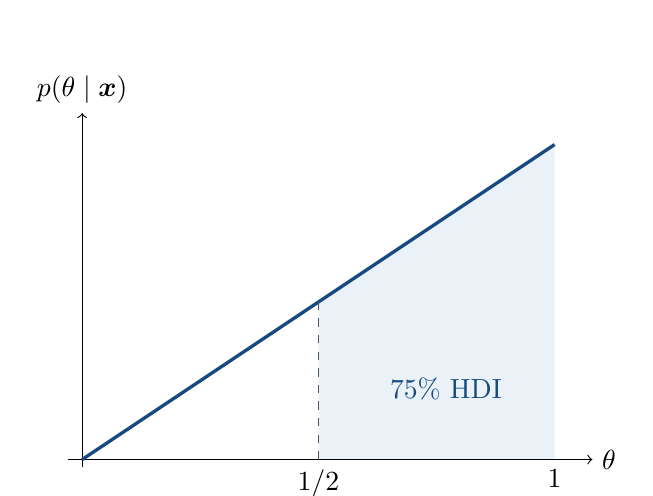
\begin{tikzpicture}[x=6cm,y=2cm]
  \fill[statlight] (0.5,0) -- (0.5,1) -- (1,2) -- (1,0) -- cycle;
  \draw[->] (-0.03,0) -- (1.08,0) node[right] {$\theta$};
  \draw[->] (0,-0.05) -- (0,2.2) node[above] {$p(\theta\given\xvec)$};
  \draw[very thick,statblue] (0,0) -- (1,2);
  \draw[dashed,statgrey] (0.5,0) -- (0.5,1);
  \node[below] at (0.5,0) {$1/2$};
  \node[below] at (1,0) {$1$};
  \node[statblue] at (0.77,0.45) {75\% HDI};
\end{tikzpicture}
\end{center}

Every included point has density at least as large as every excluded point,
so $[1/2,1]$ is a highest-density interval. Equivalently, among intervals
$[a,b]$ satisfying $b^2-a^2=0.75$, its width
$(b-a)=0.75/(a+b)$ is minimised by taking the largest possible $a+b$, namely
$b=1$ and $a=1/2$.

\subsubsection*{(c) Confidence versus credibility}

A 75\% confidence procedure has repeated-sampling coverage
\[
  \mathbb{P}_{\theta}\{L(X)\leq\theta\leq U(X)\}=0.75.
\]
The probability refers to the random interval procedure; after observing the
data, the realised frequentist interval is fixed.

A 75\% credible interval $[a,b]$ satisfies
\[
  \mathbb{P}(a\leq\theta\leq b\given\xvec)=0.75.
\]
This probability refers directly to the posterior distribution of $\theta$
given the observed data, prior, and model. Identical numerical endpoints do
not change these different interpretations.

\clearpage

\subsection{Answer 9: Gibbs sampling for a correlated bivariate normal}
\answernav{9}

\studyheading{Definitions}
The target coordinates $\theta_1,\theta_2$ have zero means, unit marginal variances, and correlation $\rho$, with $-1<\rho<1$.
A full conditional holds the other coordinate and the data $x$ fixed.
The Normal kernel $\exp\{-(u-m)^2/(2v)\}$ identifies mean $m$ and variance $v>0$.
Superscript $(t)$ labels the Gibbs sweep.

The joint density has kernel
\[
\pi(\theta_1,\theta_2\mid x)
\propto
\exp\left\{
-\frac{1}{2(1-\rho^2)}
\left(\theta_1^2-2\rho\theta_1\theta_2+\theta_2^2\right)
\right\}.
\]

\subsubsection*{(a) Full conditional distributions}

For the first full conditional,
\[
p(\theta_1\mid\theta_2,x)
=
\frac{p(\theta_1,\theta_2\mid x)}{p(\theta_2\mid x)}
\propto p(\theta_1,\theta_2\mid x)
\quad\text{as a function of }\theta_1.
\]
The denominator is constant when \(\theta_2\) and \(x\) are held fixed. Thus
the joint kernel is sufficient: terms involving \(\theta_1\) must be kept,
while terms free of \(\theta_1\) may be absorbed into the proportionality
constant.

We aim to match the Normal kernel
\[
\exp\left\{-\frac{(\theta_1-m)^2}{2v}\right\},
\]
where \(m\) is the mean and \(v\) is the variance. Treat the quadratic form
in the joint exponent as a quadratic in \(\theta_1\). Completing the square
gives
\begin{align*}
\theta_1^2-2\rho\theta_1\theta_2+\theta_2^2
&=(\theta_1-\rho\theta_2)^2
  -\rho^2\theta_2^2+\theta_2^2\\
&=(\theta_1-\rho\theta_2)^2
  +(1-\rho^2)\theta_2^2.
\end{align*}
Substitution into the joint kernel gives
\begin{align*}
p(\theta_1\mid\theta_2,x)
&\propto
\exp\left\{
-\frac{(\theta_1-\rho\theta_2)^2+(1-\rho^2)\theta_2^2}
{2(1-\rho^2)}
\right\}\\
&=
\exp\left\{-\frac{(\theta_1-\rho\theta_2)^2}
{2(1-\rho^2)}\right\}
\exp\left\{-\frac{\theta_2^2}{2}\right\}\\
&\propto
\exp\left\{-\frac{(\theta_1-\rho\theta_2)^2}
{2(1-\rho^2)}\right\}.
\end{align*}
The factor \(\exp(-\theta_2^2/2)\) is dropped because it is constant with
respect to \(\theta_1\). Matching the remaining expression to the Normal
kernel yields
\[
\boxed{
\theta_1\mid\theta_2,x
\sim N\left(\rho\theta_2,\,1-\rho^2\right).
}
\]
The condition \(-1<\rho<1\) ensures that the conditional variance
\(1-\rho^2\) is positive.

For the other coordinate, the same calculation gives
\[
\theta_2^2-2\rho\theta_1\theta_2+\theta_1^2
=
(\theta_2-\rho\theta_1)^2+(1-\rho^2)\theta_1^2.
\]
Hence, by symmetry,
\[
\boxed{
\theta_2\mid\theta_1,x
\sim N\left(\rho\theta_1,\,1-\rho^2\right).
}
\]

\subsubsection*{(b) Gibbs sampler}

Starting from any valid pair
\((\theta_1^{(0)},\theta_2^{(0)})\in\mathbb{R}^2\), repeat for
\(t=1,\ldots,T\):
\begin{enumerate}
    \item Draw
    \[
    \theta_1^{(t)}
    \sim N\left(\rho\theta_2^{(t-1)},\,1-\rho^2\right).
    \]
    \item Draw
    \[
    \theta_2^{(t)}
    \sim N\left(\rho\theta_1^{(t)},\,1-\rho^2\right).
    \]
    \item Store \((\theta_1^{(t)},\theta_2^{(t)})\).
\end{enumerate}

Each update is sampled directly from a full conditional distribution, so no
accept--reject step is required.

\subsubsection*{(c) Equilibrium and independence}

If the chain is started in equilibrium, every stored pair has the required
joint distribution. The pairs are nevertheless generally \emph{not}
independent, because the distribution of the next pair depends on the current
pair through the Gibbs updates.

When $\rho=0$, the coordinates are independent and fresh conditional draws produce independent pairs across full sweeps. This exception does not apply to a correlated target.

\subsubsection*{(d) Effect of strong correlation}

When \(\rho\) is close to \(1\), the joint density is concentrated around the
diagonal \(\theta_1=\theta_2\), while the conditional variance
\[
1-\rho^2
\]
is close to zero. Each Gibbs update therefore makes only a small move along
the narrow high-density region. This produces strong autocorrelation and slow
mixing. Thus, although every Gibbs proposal is accepted, an acceptance rate of
one does not imply efficient exploration of the target distribution.

\clearpage

\subsection{Answer 10: Metropolis--Hastings with an asymmetric-proposal extension}
\answernav{10}

\studyheading{Definitions}
The target is proportional to $\theta^2e^{-\theta}$ on $\theta>0$ and is zero otherwise.
Let $q(\theta^*\given\theta)$ be the proposal density, $\alpha(\theta,\theta^*)$ the acceptance probability, and $(t)$ the iteration index.
The proposal $N(\theta,s^2)$ has variance $s^2>0$, fixed across states and iterations; the current state must lie in the target support.

The target density has kernel
\[
\pi(\theta)\propto \theta^2e^{-\theta},
\qquad \theta>0.
\]

\subsubsection*{(a) Acceptance probability}

For a random-walk proposal
\[
\theta^*\mid\theta^{(t)}\sim N\left(\theta^{(t)},s^2\right),
\]
the proposal is symmetric:
\[
q(\theta^*\mid\theta^{(t)})
=q(\theta^{(t)}\mid\theta^*).
\]
Consequently, the proposal-density terms cancel from the
Metropolis--Hastings ratio. If \(\theta^*>0\),
\begin{align*}
\alpha\left(\theta^{(t)},\theta^*\right)
&=
\min\left\{
\frac{\pi(\theta^*)}{\pi(\theta^{(t)})},1
\right\}\\
&=
\boxed{
\min\left\{
\left(\frac{\theta^*}{\theta^{(t)}}\right)^2
\exp\left[-\left(\theta^*-\theta^{(t)}\right)\right],
1
\right\}.
}
\end{align*}
If \(\theta^*\leq 0\), then \(\pi(\theta^*)=0\), so the proposal is rejected
and \(\alpha=0\).

\subsubsection*{(b) Normalising constant}

The unknown normalising constant appears in both the numerator and denominator
of the target-density ratio and therefore cancels. Only the target kernel is
needed.

\subsubsection*{(c) One sampler iteration}

One iteration of the algorithm is:
\begin{enumerate}
    \item Generate a proposal
    \[
    \theta^*\sim N\left(\theta^{(t)},s^2\right).
    \]
    \item Calculate \(\alpha(\theta^{(t)},\theta^*)\) as above.
    \item Generate \(U\sim\operatorname{Uniform}(0,1)\).
    \item Set
    \[
    \theta^{(t+1)}=
    \begin{cases}
    \theta^*, & U\leq\alpha(\theta^{(t)},\theta^*),\\
    \theta^{(t)}, & U>\alpha(\theta^{(t)},\theta^*).
    \end{cases}
    \]
\end{enumerate}

\subsubsection*{(d) Proposal scale}

If \(s\) is extremely small, proposals remain close to the current state and
the acceptance rate will usually be high. However, the chain moves only in
small steps, producing high autocorrelation and slow exploration.

If \(s\) is extremely large, many proposals will be negative or will fall in
regions where the target density is very small. Most will be rejected, so the
chain will repeatedly remain at the same state and again mix slowly.

\subsubsection*{(e) Asymmetric proposals}

For an asymmetric proposal, the proposal terms do not cancel. The acceptance
probability becomes
\[
\boxed{
\alpha(\theta,\theta^*)
=
\min\left\{
\frac{\pi(\theta^*)q(\theta\mid\theta^*)}
{\pi(\theta)q(\theta^*\mid\theta)},
1
\right\}.
}
\]
The additional factor is therefore
\[
\boxed{
\frac{q(\theta\mid\theta^*)}{q(\theta^*\mid\theta)},
}
\]
that is, the reverse-proposal density divided by the forward-proposal density.

\clearpage

\subsection{Answer 11: Bayes factors and posterior odds}
\answernav{11}

\studyheading{Definitions}
$M_0$ fixes $\theta=1/2$; $M_1$ assigns $\theta\sim\operatorname{Beta}(1,1)$.
Write $m_j(x)=\mathbb P(X=x\given M_j)$ for the marginal likelihood and $B_{10}=m_1(x)/m_0(x)$ for the Bayes factor favouring $M_1$.
The Beta integral is $B(a,b)=\int_0^1u^{a-1}(1-u)^{b-1}\,du$.
Prior probabilities of the two models are distinct from their priors for $\theta$.

\subsubsection*{(a) Marginal likelihoods}

Under \(M_0\), the marginal probability of observing \(X=x\) is
\[
m_0(x)
=
\mathbb{P}(X=x\mid M_0)
=
\binom{n}{x}\left(\frac12\right)^x
\left(\frac12\right)^{n-x}
=
\boxed{\binom{n}{x}2^{-n}}.
\]

Under \(M_1\), integrate the likelihood with respect to the uniform prior:
\begin{align*}
m_1(x)
&=
\mathbb{P}(X=x\mid M_1)\\
&=
\binom{n}{x}
\int_0^1\theta^x(1-\theta)^{n-x}\,d\theta\\
&=
\binom{n}{x}B(x+1,n-x+1)\\
&=
\binom{n}{x}
\frac{x!(n-x)!}{(n+1)!}\\
&=
\boxed{\frac{1}{n+1}}.
\end{align*}

\subsubsection*{(b) Bayes factor}

The Bayes factor in favour of \(M_1\) over \(M_0\) is
\[
\boxed{
B_{10}
=
\frac{m_1(x)}{m_0(x)}
=
\frac{2^n}{(n+1)\binom{n}{x}}.
}
\]
Values greater than one favour \(M_1\), while values less than one favour
\(M_0\).

\subsubsection*{(c) Posterior model odds}

Posterior odds equal the Bayes factor multiplied by prior odds:
\[
\boxed{
\frac{\mathbb{P}(M_1\mid x)}{\mathbb{P}(M_0\mid x)}
=
B_{10}
\frac{\mathbb{P}(M_1)}{\mathbb{P}(M_0)}.
}
\]

\subsubsection*{(d) Numerical comparison}

For \(n=3\) and \(x=3\),
\[
m_0(3)=\frac18,
\qquad
m_1(3)=\frac14,
\qquad
B_{10}=2.
\]
Thus the observed data are twice as probable under \(M_1\) as under \(M_0\),
so the data favour \(M_1\).

If
\[
\mathbb{P}(M_1)=\frac15,
\qquad
\mathbb{P}(M_0)=\frac45,
\]
then the prior odds for \(M_1\) are \(1/4\). Hence
\[
\frac{\mathbb{P}(M_1\mid x)}{\mathbb{P}(M_0\mid x)}
=2\left(\frac14\right)
=\frac12.
\]
Therefore
\[
\boxed{
\mathbb{P}(M_1\mid x)=\frac13,
\qquad
\mathbb{P}(M_0\mid x)=\frac23.
}
\]
The data favour \(M_1\), but the prior favoured \(M_0\) by four to one. The
evidence from this small sample is not strong enough to overturn that prior
preference, so \(M_0\) remains more probable a posteriori.

\clearpage

\subsection{Answer 12: Pareto likelihood and Gamma posterior}
\answernav{12}

\studyheading{Definitions}
The known lower endpoint is $m>0$, and the observed data satisfy $x_i\ge m$.
We use the shape--rate Gamma kernel
$\theta^{A-1}e^{-B\theta}$ for $\theta>0$, $A,B>0$, with mean $A/B$ and mode $(A-1)/B$ when $A>1$.
The MAP estimate is this posterior mode.
The prior $\theta e^{-\theta}$ is $\operatorname{Gamma}(2,1)$.

Since $m$ is known and the observed sample is valid, the support indicator does not depend on $\theta$.

\subsubsection*{(a) Likelihood}

By conditional independence,
\begin{align*}
L(\theta;\xvec)
&=\prod_{i=1}^n
  \left[\theta m^\theta x_i^{-(\theta+1)}\right]\\
&=\theta^n m^{n\theta}
  \prod_{i=1}^n x_i^{-(\theta+1)}.
\end{align*}
The factor $m^{n\theta}$ must be retained because it depends on $\theta$.
Using $a^b=e^{b\log a}$,
\begin{align*}
L(\theta;\xvec)
&=\theta^n
  \exp\left(n\theta\log m\right)
  \exp\left[-(\theta+1)\sum_{i=1}^n\log x_i\right]\\
&=\theta^n
  \exp\left[-\sum_{i=1}^n\log x_i\right]
  \exp\left[-\theta\left\{
    \sum_{i=1}^n\log x_i-n\log m
  \right\}\right].
\end{align*}
The first exponential in the final line does not depend on $\theta$ and may
be absorbed into the proportionality constant. Also,
\[
\sum_{i=1}^n\log x_i-n\log m
=\sum_{i=1}^n\log\left(\frac{x_i}{m}\right)
=S.
\]
Therefore,
\[
\boxed{
L(\theta;\xvec)\propto\theta^n e^{-\theta S},
\qquad \theta>0.
}
\]

\subsubsection*{(b) Posterior distribution}

Multiplying the likelihood by the prior gives
\begin{align*}
p(\theta\given\xvec)
&\propto L(\theta;\xvec)p(\theta)\\
&\propto
\theta^n e^{-\theta S}\,
\theta e^{-\theta}\\
&=\theta^{n+1}e^{-(S+1)\theta},
\qquad \theta>0.
\end{align*}
Comparing this with the shape--rate Gamma kernel
\[
\theta^{A-1}e^{-B\theta},
\]
we obtain
\[
A-1=n+1,
\qquad
B=S+1.
\]
Hence
\[
\boxed{
\theta\given\xvec
\sim\operatorname{Gamma}(n+2,S+1)
\quad\text{in shape--rate form},
\qquad \theta>0.
}
\]
Because $x_i\geq m$, each $\log(x_i/m)\geq0$, so $S+1>0$ as required.

\subsubsection*{(c) Posterior mean and MAP estimate}

For a shape--rate $\operatorname{Gamma}(A,B)$ distribution, the mean is
$A/B$. Therefore,
\[
\boxed{
\E(\theta\given\xvec)=\frac{n+2}{S+1}.
}
\]
The MAP estimate is the posterior mode. Since $A=n+2>1$,
\[
\boxed{
\widehat{\theta}_{\mathrm{MAP}}
=\frac{A-1}{B}
=\frac{n+1}{S+1}.
}
\]

\clearpage

\subsection{Answer 13: Bayesian German tank problem}
\answernav{13}

\studyheading{Definitions}
Write $x_{(1)}=\min_i x_i$ and $x_{(n)}=\max_i x_i$; $\mathbf1\{A\}$ is one when $A$ holds and zero otherwise.
Our Pareto convention is
$p(\theta)=ab^a\theta^{-a-1}\mathbf1\{\theta\ge b\}$, with shape $a>0$ and lower bound $b>0$.
$\widetilde X$ denotes a new serial number, conditionally independent of the sample given $\theta$.
We use the stated continuous, conditionally iid model with $n\ge1$ and positive observations.

Write
\[
a_n=\alpha+n,
\qquad
b_n=\max\{\beta,x_{(n)}\}.
\]

\subsubsection*{(a) Likelihood and posterior}

For observations from $\operatorname{Uniform}(0,\theta)$,
\begin{align*}
L(\theta;\xvec)
&=\prod_{i=1}^n
  \left[\frac{1}{\theta}\,
  \mathbf{1}\{0<x_i<\theta\}\right]\\
&=\theta^{-n}\,
  \mathbf{1}\{x_{(1)}>0\}
  \prod_{i=1}^n\mathbf{1}\{x_i<\theta\}\\
&=\theta^{-n}\,
  \mathbf{1}\{x_{(1)}>0\}
  \mathbf{1}\{x_{(n)}<\theta\}.
\end{align*}
For a valid observed sample, $\mathbf{1}\{x_{(1)}>0\}$ does not depend on
$\theta$. Hence
\[
L(\theta;\xvec)
\propto\theta^{-n}\mathbf{1}\{\theta>x_{(n)}\}.
\]
Multiplying by the prior gives
\begin{align*}
p(\theta\mid\xvec)
&\propto
\theta^{-n}\mathbf{1}\{\theta>x_{(n)}\}
\theta^{-(\alpha+1)}\mathbf{1}\{\theta\geq\beta\}\\
&=\theta^{-(\alpha+n+1)}
  \mathbf{1}\{\theta\geq b_n\}\\
&=\theta^{-(a_n+1)}\mathbf{1}\{\theta\geq b_n\}.
\end{align*}
The distinction between strict and non-strict inequalities at one endpoint
is irrelevant for a continuous density. Since
\[
\int_{b_n}^{\infty}\theta^{-(a_n+1)}\,d\theta
=\frac{b_n^{-a_n}}{a_n},
\]
the normalised posterior density is
\[
p(\theta\mid\xvec)
=\frac{a_n b_n^{a_n}}{\theta^{a_n+1}},
\qquad \theta\geq b_n.
\]
Therefore,
\[
\boxed{
\theta\mid\xvec
\sim\operatorname{Pareto}\!\left(
\alpha+n,\max\{\beta,x_{(n)}\}
\right).
}
\]
The data change the lower bound exactly when $x_{(n)}>\beta$. Otherwise the
lower bound remains $\beta$, although the shape still changes from $\alpha$
to $\alpha+n$.

\subsubsection*{(b) Posterior mean}

Because $a_n=\alpha+n>1$, the posterior mean exists and is
\[
\boxed{
\E(\theta\mid\xvec)
=\frac{a_n b_n}{a_n-1}
=\frac{(\alpha+n)\max\{\beta,x_{(n)}\}}
{\alpha+n-1}.
}
\]
Since $a_n/(a_n-1)>1$ and $b_n\geq x_{(n)}$,
\[
\E(\theta\mid\xvec)>b_n\geq x_{(n)}
=\widehat{\theta}_{\mathrm{MLE}}.
\]
This is sensible. The MLE is the smallest value of $\theta$ compatible with
the data because the likelihood decreases for $\theta>x_{(n)}$. Moreover,
$X_{(n)}<\theta$ almost surely and
\[
\E(X_{(n)}\mid\theta)=\frac{n}{n+1}\theta,
\]
so the sample maximum systematically falls below the true upper endpoint.
The posterior mean allows for the unobserved region above the largest captured
serial. Frequentist bias is a repeated-sampling property; the posterior mean
is instead the Bayes estimate under squared-error loss.

\subsubsection*{(c) Posterior predictive distribution}

For a new serial number $\widetilde X$,
\begin{align*}
p(\widetilde x\mid\xvec)
&=\int_{b_n}^{\infty}
  \frac{1}{\theta}\mathbf{1}\{0<\widetilde x<\theta\}
  \frac{a_n b_n^{a_n}}{\theta^{a_n+1}}\,d\theta\\
&=a_n b_n^{a_n}
  \int_{\max\{b_n,\widetilde x\}}^{\infty}
  \theta^{-(a_n+2)}\,d\theta,
  \qquad \widetilde x>0.
\end{align*}
Thus
\[
p(\widetilde x\mid\xvec)
=
\begin{cases}
\displaystyle
\frac{a_n}{a_n+1}\frac{1}{b_n},
&0<\widetilde x\leq b_n,\\[1.1em]
\displaystyle
\frac{a_n b_n^{a_n}}{(a_n+1)\widetilde x^{a_n+1}},
&\widetilde x>b_n,\\[0.8em]
0,&\widetilde x\leq0.
\end{cases}
\]
Equivalently, this is the mixture
\[
\boxed{
\frac{a_n}{a_n+1}\operatorname{Uniform}(0,b_n)
+\frac{1}{a_n+1}\operatorname{Pareto}(a_n,b_n).
}
\]
The component weights sum to one. The Uniform component has no probability
above $b_n$, whereas the Pareto component lies above $b_n$ almost surely.
Therefore,
\[
\boxed{
\mathbb{P}(\widetilde X>b_n\mid\xvec)
=\frac{1}{a_n+1}
=\frac{1}{\alpha+n+1}.
}
\]
This is the posterior predictive probability that the next captured serial
exceeds whichever is larger: the confirmed lower bound $\beta$ or the current
sample maximum.

\subsubsection*{(d) Why there is no contradiction with the
Pitman--Koopman--Darmois theorem}

In a regular exponential-family model, the support cannot change with the
parameter: a representation of the form
\[
p(x\mid\theta)
=b(x)\frac{\exp\{c(\theta)T(x)\}}{a(\theta)}
\]
has support determined by $b(x)$, since the exponential term is positive.
For the Uniform model,
\[
p(x\mid\theta)=\frac{1}{\theta}
\mathbf{1}\{0<x<\theta\},
\]
and the indicator switches on or off as $\theta$ changes. Its support depends
on $\theta$, so this is an irregular model rather than a regular exponential
family.

The Pitman--Koopman--Darmois theorem assumes, among other regularity
conditions, parameter-independent support. This model violates that
assumption and lies outside the theorem's scope. It may therefore have the
fixed-dimensional sufficient statistic $x_{(n)}$ and a conjugate prior without
being an exponential family. The existence of a conjugate prior does not by
itself imply exponential-family structure.

\subsubsection*{(e) Numerical posterior and 95\% HPD interval}

Here $n=4$, $x_{(n)}=60$, $\alpha=1$, and $\beta=50$, so
\[
a_n=5,
\qquad
b_n=60,
\qquad
\theta\mid\xvec\sim\operatorname{Pareto}(5,60).
\]
The posterior mean is
\[
\boxed{
\E(\theta\mid\xvec)=\frac{5(60)}{4}=75.
}
\]
The posterior density is strictly decreasing on $[60,\infty)$, so its
highest-density interval must begin at the posterior mode and lower support
boundary, $60$. If the upper endpoint is $u$, then
\[
0.05
=\mathbb{P}(\theta>u\mid\xvec)
=\left(\frac{60}{u}\right)^5.
\]
Hence
\[
u=60(20)^{1/5}\approx109.2,
\]
and
\[
\boxed{
\text{95\% HPD interval}
=\left[60,\,60(20)^{1/5}\right]
\approx[60,109.2].
}
\]
The lower endpoint is $60$ because values below the largest observed serial
are impossible, and the decreasing posterior density is maximised at that
boundary.

\clearpage

\subsection{Answer 14: Marginal and conditional distributions}
\answernav{14}

\studyheading{Definitions}
Let $\xvec$ be the observed data and $p(\theta_1,\theta_2\given\xvec)$ a proper joint posterior.
A \emph{marginal} integrates out an unreported coordinate; a \emph{full conditional} holds every other coordinate fixed.
Conditional-density ratios below are used only where $p(\theta_2\given\xvec)>0$.
The symbol $u$ is a dummy integration variable; whether $\theta_2$ is integrated out or held fixed distinguishes the two calculations.

The marginal posterior
\[
p(\theta_1\mid\xvec)
\]
conditions only on the observed data. It describes uncertainty about
$\theta_1$ while averaging over all possible values of $\theta_2$. It is
obtained by integrating $\theta_2$ out of the joint posterior:
\[
\boxed{
p(\theta_1\mid\xvec)
=\int p(\theta_1,\theta_2\mid\xvec)\,d\theta_2.
}
\]

The full conditional posterior
\[
p(\theta_1\mid\theta_2,\xvec)
\]
conditions on both the data and a specified value of $\theta_2$. By the
definition of conditional density,
\begin{align*}
p(\theta_1\mid\theta_2,\xvec)
&=\frac{p(\theta_1,\theta_2\mid\xvec)}
{p(\theta_2\mid\xvec)}\\
&=\boxed{
\frac{p(\theta_1,\theta_2\mid\xvec)}
{\int p(u,\theta_2\mid\xvec)\,du}
}.
\end{align*}
Equivalently, when viewed as a function of $\theta_1$,
\[
p(\theta_1\mid\theta_2,\xvec)
\propto p(\theta_1,\theta_2\mid\xvec),
\]
because the normalising denominator is constant with respect to $\theta_1$.
Thus marginalisation averages over the other parameter, whereas conditioning
holds it fixed. Full conditionals are the distributions used for Gibbs
updates.

\clearpage

\subsection{Answer 15: Prior beliefs and conflicting data}
\answernav{15}

\studyheading{Definitions}
Let $L(\theta;\xvec)=p(\xvec\given\theta)$ and let
$m(\xvec)=\int L(\theta;\xvec)p(\theta)\,d\theta$ be the marginal likelihood.
Bayes' update is $p(\theta\given\xvec)=L(\theta;\xvec)p(\theta)/m(\xvec)$, provided $0<m(\xvec)<\infty$.
The prior here excludes the entire region $\theta>1/2$, not merely a single value.

The reasoning is incorrect. The prior density is zero for every
$\theta>1/2$. Bayes' theorem gives
\[
p(\theta\mid\xvec)
\propto p(\xvec\mid\theta)p(\theta),
\]
so
\[
p(\theta\mid\xvec)=0
\qquad\text{whenever }\theta>1/2.
\]
Hence
\[
\boxed{
\mathbb{P}(\theta>1/2\mid\xvec)=0.
}
\]
This remains true regardless of how many observations are collected. The
likelihood can redistribute posterior mass only among parameter values to
which the prior assigns positive density; it cannot create support in a
region excluded by the prior.

The observed proportion $80/100=0.8$ instead reveals serious conflict between
the data and the assumed model--prior combination. The researcher should
reconsider the restricted prior, or investigate whether the Bernoulli model
is appropriate. With the restriction left unchanged, additional data cannot
make the posterior probability above $1/2$ positive.

\clearpage

\subsection{Answer 16: Interpreting identical interval endpoints}
\answernav{16}

\studyheading{Definitions}
$C(X)$ denotes an interval computed from a random sample $X$; $C(\xvec)$ is its realised value.
$\mathbb P_\theta$ describes repeated sampling with $\theta$ fixed.
In contrast, $\mathbb P(\,\cdot\mid\xvec)$ for the parameter is calculated from its posterior under the chosen model and prior.
The stated 95\% levels refer respectively to coverage and posterior probability.

For the Bayesian interval,
\[
\boxed{
\mathbb{P}(0.3\leq\theta\leq0.6\mid\xvec)=0.95.
}
\]
Conditional on the observed data, the assumed model, and the prior, there is
95\% posterior probability that $\theta$ lies between $0.3$ and $0.6$. The
observed data are fixed, while uncertainty about $\theta$ is represented by
its posterior distribution.

For a frequentist 95\% confidence-interval procedure $C(X)$,
\[
\boxed{
\mathbb{P}_{\theta}\{\theta\in C(X)\}=0.95.
}
\]
Here $\theta$ is fixed and the interval is random because it is calculated
from the random sample $X$. Under repeated sampling at the same true value of
$\theta$, 95\% of the intervals generated by the procedure would contain
$\theta$. Once the data have been observed, the realised interval is fixed;
the frequentist statement is not that this particular interval contains
$\theta$ with probability 0.95.

Therefore identical endpoints do not imply identical interpretations. The
credible interval assigns posterior probability to values of $\theta$ given
the observed data, whereas the confidence interval describes the long-run
coverage of a random interval-producing procedure.

\clearpage

\subsection{Answer 17: Choosing a conjugate prior}
\answernav{17}

\studyheading{Definitions}
A prior family is \emph{conjugate} when multiplication by the likelihood and normalisation return a member of that family.
For the example below, the Binomial likelihood kernel is $\theta^x(1-\theta)^{n-x}$ and the Beta prior kernel is $\theta^{a-1}(1-\theta)^{b-1}$ on $(0,1)$, with $a,b>0$.
A valid posterior requires a finite, positive normalising integral.

For example, multiplying the Binomial and Beta kernels adds their success and failure exponents. Thus
\[
X\mid\theta\sim\operatorname{Bin}(n,\theta),
\qquad
\theta\sim\operatorname{Beta}(a,b)
\]
implies
\[
\theta\mid X=x
\sim\operatorname{Beta}(a+x,b+n-x).
\]
One practical advantage is that posterior updating reduces to updating the
hyperparameters. Posterior summaries and predictive calculations can often be
obtained analytically, without numerical integration.

A nonconjugate prior does not make the analysis invalid. It may be preferable
when it represents the available prior information more faithfully. However,
the posterior may not have a standard form, and its normalising constant or
required expectations may be difficult to calculate. Numerical quadrature,
grid approximation, importance sampling, or MCMC may then be required.

\clearpage

\subsection{Answer 18: Equilibrium and independence}
\answernav{18}

\studyheading{Definitions}
An invariant or equilibrium distribution is preserved by the chain's transition.
Starting from it makes the chain \emph{stationary}: every iteration has the same marginal target distribution.
This is weaker than independence across iterations.
Here one Gibbs sweep updates each coordinate once from its exact full conditional, using the newest available conditioning value.

To see invariance directly, start with a pair having density
$p(\theta_1,\theta_2\given\xvec)$. Updating $\theta_1$ while leaving
$\theta_2$ unchanged gives density
\[
p(\theta_2\given\xvec)\,
p(\theta_1'\given\theta_2,\xvec)
=p(\theta_1',\theta_2\given\xvec).
\]
The second conditional update reconstructs the same joint density in
the same way. Therefore the full sweep preserves the target.
Starting at equilibrium guarantees stationarity. If
\[
(\theta_1^{(0)},\theta_2^{(0)})
\sim p(\theta_1,\theta_2\mid\xvec),
\]
then
\[
\boxed{
(\theta_1^{(t)},\theta_2^{(t)})
\sim p(\theta_1,\theta_2\mid\xvec)
\quad\text{for every }t\geq0.
}
\]
Thus no convergence from an incorrectly distributed initial state is needed.

Independence does not follow. A systematic Gibbs update has the form
\[
\theta_1^{(t+1)}
\sim p(\theta_1\mid\theta_2^{(t)},\xvec),
\]
followed by
\[
\theta_2^{(t+1)}
\sim p(\theta_2\mid\theta_1^{(t+1)},\xvec).
\]
The new pair is generated using components of the current pair, so successive
states are generally serially dependent. This dependence can be particularly
strong when the target parameters are strongly correlated. Starting at
equilibrium gives the correct marginal distribution at every iteration, but
it does not turn the Markov chain into independent posterior draws.

\clearpage

\subsection{Answer 19: Assessing a Metropolis--Hastings sampler}
\answernav{19}

\studyheading{Definitions}
The \emph{acceptance rate} is the fraction of proposed moves accepted.
\emph{Autocorrelation} measures dependence between draws at different lags.
For a chosen posterior summary, \emph{effective sample size} is the number of independent target draws giving comparable Monte Carlo precision.
Efficiency concerns that precision per unit of computation, not the acceptance fraction alone.

An acceptance rate of 99\% does not by itself demonstrate efficiency. With a
very small proposal standard deviation, proposed values lie close to the
current state. The target density changes little across such a short move, so
most proposals are accepted; however, each accepted move advances the chain
only a small distance.

The expected consequences are slow exploration of the posterior and strong
autocorrelation between successive draws. A large recorded sample may then
contain information equivalent to a much smaller independent sample.

In addition to acceptance rate, useful diagnostics include:
\begin{itemize}
  \item a trace plot, to assess whether the chain explores the full target
        region;
  \item the autocorrelation function, to measure serial dependence; and
  \item the effective sample size, to quantify the independent information
        represented by the chain.
\end{itemize}
Thus a very high acceptance rate may indicate that the proposal scale is too
small, not that the sampler is highly efficient.

An exact independent draw from the target would also have acceptance probability one and would be efficient. High acceptance is therefore neither sufficient evidence of efficiency nor inherently a fault; the movement and dependence matter.

\clearpage

\subsection{Answer 20: Estimation and prediction}
\answernav{20}

\studyheading{Definitions}
$\mu$ is the population mean and $\widetilde X$ is a new observation.
Write $\mu\given\xvec\sim N(m_n,v_n)$, where $v_n$ is the posterior variance.
The known observation variance is $\sigma^2>0$; conditional on $\mu$, the new Normal observation is independent of the original sample.
A predictive distribution averages over parameter uncertainty as well as new-observation noise.

The posterior distribution
\[
p(\mu\mid\xvec)
\]
describes remaining uncertainty about the unknown population mean $\mu$ after
observing the data. The posterior predictive distribution
\[
p(\widetilde x\mid\xvec)
=\int p(\widetilde x\mid\mu)
p(\mu\mid\xvec)\,d\mu
\]
describes uncertainty about a future observation $\widetilde X$. It includes
both uncertainty about $\mu$ and the new observation's sampling variation
around $\mu$.

If
\[
\mu\mid\xvec\sim\mathcal{N}(m_n,v_n),
\]
then
\[
\boxed{
\widetilde X\mid\xvec
\sim\mathcal{N}(m_n,\sigma^2+v_n).
}
\]
As $n\to\infty$, under the model and standard regularity conditions,
\[
v_n\longrightarrow0.
\]
Hence posterior uncertainty about $\mu$ approaches zero. By contrast,
\[
\operatorname{Var}(\widetilde X\mid\xvec)
=\underbrace{\sigma^2}_{\text{new-observation noise}}
+\underbrace{v_n}_{\text{parameter uncertainty}}
\longrightarrow\sigma^2.
\]
Predictive uncertainty therefore does not vanish: even if $\mu$ were known
exactly, a future measurement would still vary randomly around it.

\clearpage

\subsection{Answer 21: Evidence and posterior model probabilities}
\answernav{21}

\studyheading{Definitions}
The Bayes factor is
$B_{10}=p(\xvec\given M_1)/p(\xvec\given M_0)$.
Odds in favour of $M_1$ are $\mathbb P(M_1)/\mathbb P(M_0)$, with the analogous conditional ratio for posterior odds.
The two models exhaust the comparison, so their probabilities sum to one.
Here $B_{10}=4$ and the prior odds are $1:9$.

A Bayes factor updates prior model odds according to
\[
\frac{\mathbb{P}(M_1\mid\xvec)}{\mathbb{P}(M_0\mid\xvec)}
=B_{10}
\frac{\mathbb{P}(M_1)}{\mathbb{P}(M_0)}.
\]
Because $M_0$ was initially nine times as probable as $M_1$, the prior odds
in favour of $M_1$ are
\[
\frac{\mathbb{P}(M_1)}{\mathbb{P}(M_0)}=\frac19.
\]
With $B_{10}=4$, the posterior odds become
\[
\boxed{
\frac{\mathbb{P}(M_1\mid\xvec)}{\mathbb{P}(M_0\mid\xvec)}
=4\left(\frac19\right)=\frac49.
}
\]
Therefore,
\[
\mathbb{P}(M_1\mid\xvec)=\frac4{13},
\qquad
\mathbb{P}(M_0\mid\xvec)=\frac9{13}.
\]
The data favour $M_1$ relative to the prior because $B_{10}>1$, but the
evidence is not strong enough to overcome the initial nine-to-one odds in
favour of $M_0$. Thus
\[
\boxed{
\mathbb{P}(M_0\mid\xvec)>
\mathbb{P}(M_1\mid\xvec).
}
\]
The researcher's conclusion is therefore incorrect: a Bayes factor favouring
$M_1$ does not necessarily make $M_1$ the more probable model a posteriori.

\clearpage

\subsection{Answer 22: Advertising responses and Dirichlet inference}
\answernav{22}

\studyheading{Definitions}
Let $D$ be the observed table and $\mathbf p$ its six population cell probabilities.
The labels $M,F$ denote male and female; $N,U,P$ denote negative, neutral, and positive.
With parameters $a_1,\ldots,a_K>0$, a Dirichlet density has kernel
$\prod_k p_k^{a_k-1}$ on the simplex $p_k>0$, $\sum_kp_k=1$.
The joint MAP maximises this density over the entire simplex, not a one-component marginal density.

\textbf{(a) Posterior distribution.}
Write the counts in the stated order as
\[
\mathbf x=(8,6,16,12,4,14),\qquad n=60.
\]
The multinomial likelihood is
\[
L(\mathbf p;D)=\frac{60!}{\prod_{k=1}^{6}x_k!}
\prod_{k=1}^{6}p_k^{x_k}
\propto\prod_{k=1}^{6}p_k^{x_k}.
\]
The Dirichlet prior has kernel $\prod_k p_k^{1-1}=1$ on the simplex.
Consequently,
\[
p(\mathbf p\mid D)\propto
\prod_{k=1}^{6}p_k^{x_k+1-1},
\]
which is the Dirichlet kernel with parameters $x_k+1$. Thus
\[
\boxed{\mathbf p\mid D\sim\operatorname{Dirichlet}(9,7,17,13,5,15).}
\]
Its density is supported on the simplex $p_k>0$, $\sum_{k=1}^6p_k=1$;
the boundary has probability zero. The posterior concentration is
\[
A=9+7+17+13+5+15=66.
\]

\textbf{(b) Posterior mean and MAP.}
For a Dirichlet vector with parameters $a_1,\ldots,a_K$ and
$A=\sum_k a_k$,
\[
\E(p_k)=\frac{a_k}{A},\qquad
\widehat p_{k,\mathrm{MAP}}=\frac{a_k-1}{A-K}
\quad\text{when every }a_k>1.
\]
Here every posterior parameter exceeds one, so
\[
\boxed{\E(p_{MP}\mid D)=\frac{17}{66}\approx0.2576,}
\qquad
\boxed{\widehat p_{MP,\mathrm{MAP}}=
\frac{17-1}{66-6}=\frac{16}{60}\approx0.2667.}
\]
The MAP component is taken from the mode of the joint posterior for
$\mathbf p$. Since the prior density is constant on the simplex, maximising
the posterior is equivalent to maximising the likelihood, giving the observed
cell proportions.

\textbf{(c) Predicting a positive response.}
Conditional on $\mathbf p$, the probability of a positive response is
$p_{MP}+p_{FP}$. Averaging over posterior uncertainty gives
\[
\begin{aligned}
\mathbb{P}(\text{positive}\mid D)
&=\int (p_{MP}+p_{FP})p(\mathbf p\mid D)\,d\mathbf p\\
&=\E(p_{MP}+p_{FP}\mid D)\\
&=\frac{17}{66}+\frac{15}{66}
=\boxed{\frac{16}{33}\approx0.4848.}
\end{aligned}
\]
Prediction uses posterior averaging, not substitution of the MAP estimate.

\textbf{(d) Conditioning on the new person being female.}
First calculate the two relevant posterior predictive probabilities:
\[
\mathbb{P}(\text{female and positive}\mid D)=\E(p_{FP}\mid D)=\frac{15}{66},
\]
\[
\mathbb{P}(\text{female}\mid D)
=\E(p_{FN}+p_{FU}+p_{FP}\mid D)
=\frac{13+5+15}{66}=\frac{33}{66}.
\]
By the definition of conditional probability,
\[
\boxed{
\mathbb{P}(\text{positive}\mid\text{female},D)
=\frac{15/66}{33/66}=\frac5{11}\approx0.4545.
}
\]
By contrast, the joint probability is
\[
\boxed{\mathbb{P}(\text{female and positive}\mid D)
=\frac{15}{66}=\frac5{22}\approx0.2273.}
\]
The conditional probability restricts attention to the female row; the joint
probability refers to both events occurring for a person sampled from the
whole population.

\textbf{(e) Posterior dependence.}
No. The probabilities must satisfy $\sum_k p_k=1$ exactly. Increasing one
component leaves less total probability for the others. More formally, if
they were independent, then
\[
0=\operatorname{Var}\!\left(\sum_{k=1}^{6}p_k\,\middle|\,D\right)
=\sum_{k=1}^{6}\operatorname{Var}(p_k\mid D)>0,
\]
a contradiction, since each component has positive posterior variance.
Indeed, distinct Dirichlet components have
\[
\operatorname{Cov}(p_j,p_k\mid D)
=-\frac{a_ja_k}{A^2(A+1)}<0,\qquad j\ne k.
\]

\begin{keyresult}
Add counts to the Dirichlet parameters; average probabilities for prediction;
and distinguish a joint cell probability from a probability conditional on a row.
\end{keyresult}

\clearpage

\subsection{Answer 23: Rat-tumour studies and hierarchical shrinkage}
\answernav{23}

\studyheading{Definitions}
Study $j$ has observed count $y_j$, known size $n_j$, and unknown rate $\theta_j$; $\alpha,\beta>0$ are shared hyperparameters.
A $\operatorname{Beta}(\alpha,\beta)$ density is
$\theta^{\alpha-1}(1-\theta)^{\beta-1}/B(\alpha,\beta)$ on $(0,1)$, where $B(a,b)=\int_0^1u^{a-1}(1-u)^{b-1}\,du$.
$\operatorname{Exp}(1)$ uses rate one.
Partial pooling allows different study rates linked through a common population distribution.

\studyheading{Assumptions}
The hierarchy assumes conditional independence of studies given their rates, and iid Beta rates given $\alpha,\beta$.
Thus its joint density factors as
$p(\alpha)p(\beta)\prod_jp(\theta_j\given\alpha,\beta)p(y_j\given\theta_j)$,
with independent rate-one exponential hyperpriors.
Only in part (b) are the hyperparameters fixed at the supplied values.

\textbf{(a) Full conditional for a study rate.}
Holding $\alpha,\beta$ fixed, the factors involving $\theta_j$ are
\[
\begin{aligned}
p(\theta_j\mid\alpha,\beta,\mathbf y)
&\propto p(y_j\mid\theta_j)p(\theta_j\mid\alpha,\beta)\\
&\propto\theta_j^{y_j}(1-\theta_j)^{n_j-y_j}
\theta_j^{\alpha-1}(1-\theta_j)^{\beta-1}\\
&=\theta_j^{\alpha+y_j-1}(1-\theta_j)^{\beta+n_j-y_j-1}.
\end{aligned}
\]
Therefore
\[
\boxed{\theta_j\mid\alpha,\beta,\mathbf y
\sim\operatorname{Beta}(\alpha+y_j,\beta+n_j-y_j),\qquad 0<\theta_j<1.}
\]
Conditional on the hyperparameters and data, the study rates are independent.
Other studies' observations affect this study's marginal posterior through
learning $\alpha,\beta$, not through an additional factor in this full conditional.

\textbf{(b) Posterior means and shrinkage.}
For fixed $\alpha=2$, $\beta=8$, the population mean is
\[
\frac{\alpha}{\alpha+\beta}=\frac2{10}=0.2.
\]
The two posteriors are
\[
\theta_1\mid\alpha=2,\beta=8,\mathbf y\sim\operatorname{Beta}(6,14),
\]
\[
\theta_2\mid\alpha=2,\beta=8,\mathbf y\sim\operatorname{Beta}(42,68).
\]
Thus their posterior means are
\[
\boxed{\E(\theta_1\mid\alpha=2,\beta=8,\mathbf y)=\frac6{20}=0.3,}
\]
\[
\boxed{\E(\theta_2\mid\alpha=2,\beta=8,\mathbf y)=\frac{42}{110}
\approx0.3818.}
\]
To see the shrinkage explicitly, write
\[
\frac{\alpha+y_j}{\alpha+\beta+n_j}
=\frac{\alpha+\beta}{\alpha+\beta+n_j}
\frac{\alpha}{\alpha+\beta}
+\frac{n_j}{\alpha+\beta+n_j}\frac{y_j}{n_j}.
\]
Both sample proportions equal $0.4$, but study 1 puts weight $10/20=1/2$
on the population mean, whereas study 2 puts only $10/110=1/11$ on it.
The smaller study therefore experiences stronger shrinkage toward $0.2$.
The larger study has more information about its own rate, so its posterior
mean remains closer to its observed proportion.

\textbf{(c) Integrating out the study rates.}
For one study, retain the normalising factor of the Beta density:
\[
\begin{aligned}
\mathbb{P}(Y_j=y_j\mid\alpha,\beta)
&=\int_0^1 p(y_j\mid\theta_j)p(\theta_j\mid\alpha,\beta)\,d\theta_j\\
&=\binom{n_j}{y_j}\frac1{B(\alpha,\beta)}
\int_0^1\theta_j^{y_j+\alpha-1}
(1-\theta_j)^{n_j-y_j+\beta-1}\,d\theta_j\\
&=\boxed{\binom{n_j}{y_j}
\frac{B(\alpha+y_j,\beta+n_j-y_j)}{B(\alpha,\beta)}.}
\end{aligned}
\]
This is a Beta--Binomial marginal distribution, with
$y_j\in\{0,\ldots,n_j\}$.

The independent rate-one exponential hyperpriors give
\[
p(\alpha,\beta)=e^{-\alpha-\beta},\qquad \alpha>0,\quad\beta>0.
\]
The studies remain independent conditional on the hyperparameters after
their individual rates have been integrated out. Consequently,
\[
\begin{aligned}
p(\alpha,\beta\mid\mathbf y)
&\propto p(\alpha,\beta)
\prod_{j=1}^{J}\mathbb{P}(Y_j=y_j\mid\alpha,\beta)\\
&\propto e^{-(\alpha+\beta)}
\prod_{j=1}^{J}
\frac{B(\alpha+y_j,\beta+n_j-y_j)}{B(\alpha,\beta)}.
\end{aligned}
\]
Hence
\[
\boxed{
p(\alpha,\beta\mid\mathbf y)
\propto e^{-(\alpha+\beta)}B(\alpha,\beta)^{-J}
\prod_{j=1}^{J}B(\alpha+y_j,\beta+n_j-y_j),
\quad \alpha,\beta>0.
}
\]
The binomial coefficients can be dropped because the observed $y_j$ and
known $n_j$ make them constant with respect to $\alpha,\beta$.
However, $1/B(\alpha,\beta)$ depends on the hyperparameters, so it must
remain. A factor constant in $\theta_j$ need not be constant in
$\alpha,\beta$.

\textbf{(d) Sharing information and hyperparameter uncertainty.}
Every study contributes to the posterior for the common population
parameters $\alpha,\beta$. That posterior then contributes to each
study-specific posterior through
\[
p(\theta_j\mid\mathbf y)
=\int_0^\infty\!\int_0^\infty
p(\theta_j\mid\alpha,\beta,\mathbf y)
p(\alpha,\beta\mid\mathbf y)\,d\alpha\,d\beta.
\]
This is partial pooling: study rates can differ, but they are connected by
a population distribution learned from all the studies. The model does not
force them to be identical, and it does not treat them as unrelated.

Replacing $\alpha,\beta$ by fixed estimates is an empirical-Bayes plug-in
analysis. It omits uncertainty about the population distribution's parameters.
For example, the law of total variance gives
\[
\begin{aligned}
\operatorname{Var}(\theta_j\mid\mathbf y)
={}&\E\!\left[
\operatorname{Var}(\theta_j\mid\alpha,\beta,\mathbf y)
\mid\mathbf y\right]\\
&+\operatorname{Var}\!\left[
\E(\theta_j\mid\alpha,\beta,\mathbf y)
\mid\mathbf y\right].
\end{aligned}
\]
The second term represents variation in the conditional mean as the
hyperparameters vary under their posterior. A plug-in calculation does not
propagate this variation and can therefore give an overly precise account
of uncertainty.

\begin{keyresult}
Conditional conjugacy does not eliminate uncertainty in the hyperparameters.
Full Bayes learns their distribution and averages over it.
\end{keyresult}

\clearpage

\subsection{Answer 24: Bayesian regression and prediction}
\answernav{24}

\studyheading{Definitions}
Write $D=(\mathbf y,X)$, $v=\sigma^2$, and
$\operatorname{SSE}=\|\mathbf y-X\widehat{\boldsymbol\beta}\|^2$.
The inverse-Gamma kernel is $v^{-a-1}e^{-b/v}$ on $v>0$.
$t_\nu(m,s)$ denotes location $m$, \emph{scale} $s$, and $\nu$ degrees of freedom: $(T-m)/s\sim t_\nu$.
A scale is not a variance; $t_{q,\nu}$ denotes the $q$ quantile of standard $t_\nu$.

\studyheading{Assumptions}
Use independent Normal errors, fixed covariates, full column rank $X$, $n>p$, positive SSE, and the reference prior
$p(\boldsymbol\beta,v)\propto1/v$ with respect to $d\boldsymbol\beta\,dv$.
These rank and residual conditions ensure a proper posterior despite the improper prior.

There are $p=2$ regression coefficients, including the intercept. Define
\[
\nu=n-p=8,\qquad
s^2=\frac{\operatorname{SSE}}{n-p}=\frac{16}{8}=2,
\qquad C=(X^\top X)^{-1}.
\]
Here $s^2$ is the residual variance estimate; it is not the posterior mean
of $\sigma^2$.

\textbf{Why the regression posterior has this form.}
The likelihood times the reference prior gives
\[
p(\boldsymbol\beta,v\given D)
\propto v^{-n/2-1}
\exp\{-\|\mathbf y-X\boldsymbol\beta\|^2/(2v)\},
\qquad v=\sigma^2>0.
\]
Expand about the least-squares estimate. The cross term vanishes because
$X^\top(\mathbf y-X\widehat{\boldsymbol\beta})=\mathbf0$, giving
\[
\|\mathbf y-X\boldsymbol\beta\|^2
=\operatorname{SSE}
+(\boldsymbol\beta-\widehat{\boldsymbol\beta})^\top
X^\top X(\boldsymbol\beta-\widehat{\boldsymbol\beta}).
\]
The second term is a Normal quadratic. At fixed $v$ it identifies
$\boldsymbol\beta\given v,D\sim
N_p(\widehat{\boldsymbol\beta},vC)$.
Its unnormalised exponential integrates to
$(2\pi v)^{p/2}|X^\top X|^{-1/2}$, which explains the $v^{p/2}$
factor in the variance marginal below.

\textbf{(a) Marginal variance posterior.}
Under the stated reference prior,
\[
\sigma^2\mid D\sim\InvGamma\left(\frac{n-p}{2},
\frac{\operatorname{SSE}}2\right).
\]
Thus
\[
\boxed{\sigma^2\mid D\sim\InvGamma(4,8),\qquad\sigma^2>0.}
\]
An $\InvGamma(a,b)$ variable has mean $b/(a-1)$ when $a>1$, so
\[
\boxed{\E(\sigma^2\mid D)=\frac8{4-1}=\frac83\approx2.6667.}
\]
For completeness, integrating the coefficient kernel out of the joint
posterior contributes a factor $(\sigma^2)^{p/2}$. Therefore
\[
p(\sigma^2\mid D)
\propto (\sigma^2)^{-(n/2+1)}(\sigma^2)^{p/2}
\exp\!\left(-\frac{\operatorname{SSE}}{2\sigma^2}\right)
=(\sigma^2)^{-5}e^{-8/\sigma^2},
\]
confirming the shape $4$, not $n/2=5$.

\textbf{(b) Slope posterior and credible interval.}
The conditional coefficient posterior is
\[
\boldsymbol\beta\mid\sigma^2,D
\sim N_2(\widehat{\boldsymbol\beta},\sigma^2 C).
\]
The slope entry of $C$ is $1/40$, so
\[
\beta_1\mid\sigma^2,D\sim N\!\left(2,\frac{\sigma^2}{40}\right).
\]
Integrating over $\sigma^2\mid D$ gives
\[
\boxed{\beta_1\mid D\sim t_8\!\left(2,\sqrt{\frac2{40}}\right)
=t_8(2,\sqrt{0.05}).}
\]
Equivalently, $(\beta_1-2)/\sqrt{0.05}\mid D\sim t_8$. The equal-tailed
95\% credible interval is therefore
\[
2\pm2.306\sqrt{0.05}=2\pm0.5156,
\qquad\boxed{(1.484,\,2.516).}
\]
The second argument of $t_8$ is a scale, not a variance. There is no
additional division by $\sqrt n$: sample-size information is already in $C$.

\textbf{(c) Mean response versus a new observation at $x_*=0$.}
For a general predictor value, set $\mathbf z_*=(1,x_*)^\top$ and write
\[
m_*=\mathbf z_*^\top\widehat{\boldsymbol\beta},
\qquad h(x_*)=\mathbf z_*^\top C\mathbf z_*.
\]
The linear-transformation rule for a normal vector gives
\[
\mu_*\mid\sigma^2,D
\sim N\bigl(m_*,\sigma^2 h(x_*)\bigr).
\]
For a new response $\widetilde Y=\mu_*+\widetilde\varepsilon$, the new
error is independent of the coefficient uncertainty conditional on
$\sigma^2,D$, and has variance $\sigma^2$. Thus
\[
\widetilde Y\mid\sigma^2,D,x_*
\sim N\bigl(m_*,\sigma^2\{1+h(x_*)\}\bigr).
\]
Integrating over the inverse-Gamma variance posterior gives
\[
\mu_*\mid D\sim t_8\bigl(m_*,s\sqrt{h(x_*)}\bigr),
\]
\[
\widetilde Y\mid D,x_*\sim t_8\bigl(m_*,s\sqrt{1+h(x_*)}\bigr).
\]
At $x_*=0$,
\[
m_*=(1,0)\begin{pmatrix}1\\2\end{pmatrix}=1,
\qquad h(0)=\frac1{10}.
\]
Therefore the unknown mean response has posterior
\[
\boxed{\mu_*\mid D\sim t_8(1,\sqrt{0.2}),}
\]
with equal-tailed 95\% credible interval
\[
1\pm2.306\sqrt{0.2}=1\pm1.0313,
\qquad\boxed{(-0.031,\,2.031).}
\]
The new observation has posterior predictive distribution
\[
\boxed{\widetilde Y\mid D,x_*=0\sim t_8(1,\sqrt{2.2}),}
\]
with equal-tailed 95\% predictive interval
\[
1\pm2.306\sqrt{2.2}=1\pm3.4204,
\qquad\boxed{(-2.420,\,4.420).}
\]
Both intervals have the same centre and use the same $t_8$ quantile.
The predictive interval is wider because a new observation includes both
uncertainty about the regression mean and fresh observational noise. That
additional noise produces the extra $1$ in $1+h(x_*)$.

\textbf{(d) Extrapolation and predictive scale.}
Using the supplied diagonal matrix,
\[
\begin{aligned}
h(x_*)&=(1,x_*)
\begin{pmatrix}1/10&0\\0&1/40\end{pmatrix}
\begin{pmatrix}1\\x_*\end{pmatrix}\\
&=\frac1{10}+\frac{x_*^2}{40}.
\end{aligned}
\]
Hence
\[
\boxed{h(0)=0.1,\qquad h(4)=0.1+\frac{16}{40}=0.5.}
\]
The corresponding predictive scales are
\[
\boxed{s_{\mathrm{pred}}(0)=\sqrt{2(1+0.1)}=\sqrt{2.2}\approx1.4832,}
\]
\[
\boxed{s_{\mathrm{pred}}(4)=\sqrt{2(1+0.5)}=\sqrt3\approx1.7321.}
\]
At $x_*=4$, the predicted centre is $1+2(4)=9$, so the predictive
distribution is $t_8(9,\sqrt3)$. Its interval is wider than at $x_*=0$
because it has the same degrees of freedom but a larger scale.

The value $4$ lies outside the observed range $[-3,3]$. Uncertainty about
the slope has a greater effect on the fitted mean farther from the centred
design, increasing $h(x_*)$. The future-error contribution is unchanged;
the increased width comes from greater parameter uncertainty in the prediction.
This calculation assumes the linear model remains appropriate beyond the
observed range; it does not account for possible failure of that model there.

\begin{keyresult}
The mean-response scale is $s\sqrt h$; the new-observation scale is
$s\sqrt{1+h}$. The extra $1$ represents new observational noise, while
$h$ measures uncertainty about the fitted mean.
\end{keyresult}

\clearpage

\subsection{Answer 25: Gibbs, Metropolis--Hastings, and Monte Carlo error}
\answernav{25}

\studyheading{Definitions}
Take the joint support to be $x,y>0$.
We use $\operatorname{Gamma}(a,b)$ in shape--rate form, with kernel
$z^{a-1}e^{-bz}$ on $z>0$.
$N_2(\mathbf m,\Sigma)$ uses a covariance matrix $\Sigma$, and $I_2$ is the $2\times2$ identity.
The estimand in (c) is the fixed target mean $\mu_Y=\E_f(Y)$; its simulation uncertainty is measured by a Monte Carlo standard error (MCSE).

\textbf{(a) Gibbs sampler.}
For the conditional distribution of $X$, fix $y>0$ and retain all factors
involving $x$:
\[
\begin{aligned}
f(x\mid y)&\propto x^3y\exp(-xy-2x-3y)\\
&\propto x^3\exp\{-(y+2)x\},\qquad x>0.
\end{aligned}
\]
The power $3=4-1$ identifies shape $4$, and the coefficient of $x$ in
the negative exponential is the rate $y+2$. Thus
\[
\boxed{X\mid Y=y\sim\operatorname{Gamma}(4,y+2).}
\]
Similarly, fixing $x>0$ gives
\[
f(y\mid x)\propto y\exp\{-(x+3)y\},\qquad y>0,
\]
and hence
\[
\boxed{Y\mid X=x\sim\operatorname{Gamma}(2,x+3).}
\]
The corresponding normalised conditional densities are
\[
f(x\mid y)=\frac{(y+2)^4}{\Gamma(4)}x^3e^{-(y+2)x},
\qquad
f(y\mid x)=\frac{(x+3)^2}{\Gamma(2)}y e^{-(x+3)y}.
\]

Choose any valid initial pair $(x^{(0)},y^{(0)})$ with both coordinates
positive. A systematic-scan Gibbs sampler is:
\begin{enumerate}[label=\arabic*.]
  \item For $t=1,\ldots,T$, draw
        \[
        X^{(t)}\sim\operatorname{Gamma}(4,Y^{(t-1)}+2).
        \]
  \item Using this newly drawn value, draw
        \[
        Y^{(t)}\sim\operatorname{Gamma}(2,X^{(t)}+3).
        \]
  \item Record the pair $(X^{(t)},Y^{(t)})$ and repeat.
\end{enumerate}
Every draw is from an exact full conditional, so there is no accept--reject
step. Each conditional update preserves the target joint distribution;
their composition therefore has $f(x,y)$ as an equilibrium distribution.
After checking convergence and allowing suitable warm-up, retained pairs
can be used to approximate target expectations. Successive pairs are
generally dependent, not iid.

\textbf{(b) Random-walk Metropolis--Hastings.}
Let the current state be $(x,y)$ with $x,y>0$. Draw an increment
\[
\boldsymbol\varepsilon\sim N_2(\mathbf 0,\sigma^2I_2)
\]
and propose
\[
(x',y')=(x,y)+\boldsymbol\varepsilon.
\]
Equivalently, the proposed state is $N_2((x,y)^\top,\sigma^2I_2)$.
The zero-mean normal distribution describes the \emph{increment}, not an
independence proposal centred at the origin.

The proposal is symmetric:
\[
q\bigl((x',y')\mid(x,y)\bigr)
=q\bigl((x,y)\mid(x',y')\bigr),
\]
because reversing the increment leaves its squared length unchanged.
Thus the proposal densities cancel from the Metropolis--Hastings ratio.
For a proposal in the positive quadrant,
\[
\begin{aligned}
r&=\frac{f(x',y')}{f(x,y)}\\
&=\frac{(x')^3y' e^{-x'y'-2x'-3y'}}{x^3y e^{-xy-2x-3y}}\\
&=\left(\frac{x'}x\right)^3\frac{y'}y
\exp\{-x'y'+xy-2(x'-x)-3(y'-y)\}.
\end{aligned}
\]
Therefore the acceptance probability is
\[
\boxed{
a\bigl((x,y),(x',y')\bigr)=
\begin{cases}
\min\{1,r\},&x'>0,\ y'>0,\\
0,&\text{otherwise}.
\end{cases}}
\]
The unknown normalising constant of $f$ cancels in the target-density ratio.

Start from a valid positive pair. For each iteration $t=1,\ldots,T$:
\begin{enumerate}[label=\arabic*.]
  \item Draw an independent $N_2(\mathbf0,\sigma^2I_2)$ increment and
        add it to $(X^{(t-1)},Y^{(t-1)})$ to obtain $(x',y')$.
  \item If either proposed coordinate is nonpositive, reject the proposal.
        Otherwise compute $a$ above and draw $U\sim U(0,1)$ independently;
        accept if $U\leq a$.
  \item On acceptance set $(X^{(t)},Y^{(t)})=(x',y')$; on rejection set
        $(X^{(t)},Y^{(t)})=(X^{(t-1)},Y^{(t-1)})$.
  \item Record the state, including repeated states caused by rejection.
\end{enumerate}
An out-of-support proposal is rejected, not repeatedly redrawn until it is
positive: such redrawing would change the proposal distribution and its
acceptance ratio. Assess convergence before using the retained output.

\textbf{(c) A 95\% confidence interval for $\E(Y)$.}
The target is the fixed number $\mu_Y=\E_f(Y)$, estimated using a Monte
Carlo average. After suitable warm-up and convergence checks, retain
$N$ consecutive values $Y_1,\ldots,Y_N$ and calculate
\[
\bar Y_N=\frac1N\sum_{t=1}^{N}Y_t.
\]
These values are generally autocorrelated, so the iid standard error
$s_Y/\sqrt N$ is not generally valid.

One practical method is \emph{batch means}. Write $N=ab$, with $a$
non-overlapping batches of length $b$, and calculate
\[
\bar Y_k^{\mathrm{batch}}=
\frac1b\sum_{t=(k-1)b+1}^{kb}Y_t,\qquad k=1,\ldots,a,
\]
\[
s_B^2=\frac1{a-1}\sum_{k=1}^{a}
\bigl(\bar Y_k^{\mathrm{batch}}-\bar Y_N\bigr)^2.
\]
With batches long relative to the chain's dependence and sufficiently many
batches, the batch averages are approximately independent and approximately
normal under the usual Markov-chain central limit conditions. An estimated
Monte Carlo standard error is
\[
\widehat{\operatorname{MCSE}}(\bar Y_N)=\frac{s_B}{\sqrt a}.
\]
An approximate 95\% confidence interval is then
\[
\boxed{\bar Y_N\ \pm\ t_{0.975,a-1}\frac{s_B}{\sqrt a}.}
\]
For large $a$, the $t$ quantile can be replaced by $1.96$. The simulation
should be long enough for the interval to be reasonably stable when the
batch length is increased.

Equivalently, for a stationary chain satisfying a central limit theorem,
\[
\sqrt N(\bar Y_N-\mu_Y)\ \xrightarrow{d}\ N(0,\tau_Y^2),
\]
where the long-run variance is
\[
\tau_Y^2=\gamma_0+2\sum_{k=1}^{\infty}\gamma_k,
\qquad \gamma_k=\operatorname{Cov}(Y_t,Y_{t+k}).
\]
Batch means estimates this variance by $\widehat\tau_Y^2=b s_B^2$, giving
the same standard error $\sqrt{\widehat\tau_Y^2/N}=s_B/\sqrt a$.

\begin{keyresult}
This interval measures Monte Carlo error in estimating $\E(Y)$.
The empirical 2.5\% and 97.5\% quantiles of the $Y_t$ values instead give
an interval for the variable $Y$; they are not a confidence interval for its mean.
\end{keyresult}

\clearpage

\subsection{Answer 26: General Beta--Binomial Gibbs sampler}
\answernav{26}

\studyheading{Definitions}
A $\operatorname{Binomial}(n,p)$ mass function is
$\binom nx p^x(1-p)^{n-x}$ for $x=0,\ldots,n$.
A $\operatorname{Beta}(a,b)$ density has kernel
$\theta^{a-1}(1-\theta)^{b-1}$ on $(0,1)$ and normalising integral $B(a,b)$.
Here $n$ is a known positive integer and $\alpha,\beta>0$.
A full conditional treats the other variable as fixed; $(t)$ indexes complete Gibbs sweeps.

\textbf{(i) Conditional distribution of $X\mid\theta$.}
For fixed $0<\theta<1$, factor the joint kernel as
\[
f(x,\theta)\propto
\underbrace{\theta^{\alpha-1}(1-\theta)^{\beta-1}}_{\text{constant in }x}
\binom nx\theta^x(1-\theta)^{n-x}.
\]
The first factor can be dropped when finding the conditional distribution
of $X$, but $\binom nx$ must remain because it depends on $x$. Thus
\[
f(x\mid\theta)\propto\binom nx\theta^x(1-\theta)^{n-x},
\qquad x=0,1,\ldots,n.
\]
This is the Binomial kernel, so
\[
\boxed{X\mid\theta\sim\operatorname{Binomial}(n,\theta).}
\]
Indeed, the displayed Binomial probabilities already sum to one by the
binomial theorem. At the endpoints the corresponding conditional is
degenerate at $0$ or $n$; these endpoints have zero probability under the
continuous Beta marginal.

\textbf{(ii) Conditional distribution of $\theta\mid X=x$.}
Now fix $x$. The binomial coefficient is constant with respect to $\theta$,
giving
\[
f(\theta\mid x)\propto
\theta^{x+\alpha-1}(1-\theta)^{n-x+\beta-1},\qquad 0<\theta<1.
\]
Matching the exponents to a Beta density yields
\[
\boxed{\theta\mid X=x\sim
\operatorname{Beta}(\alpha+x,\beta+n-x).}
\]
Both shape parameters are positive because $\alpha,\beta>0$ and
$0\leq x\leq n$.

\textbf{Normalisation check.}
Summing the joint kernel over $x$ gives
\[
\begin{aligned}
\sum_{x=0}^{n}\binom nx
\theta^{x+\alpha-1}(1-\theta)^{n-x+\beta-1}
&=\theta^{\alpha-1}(1-\theta)^{\beta-1}
\sum_{x=0}^{n}\binom nx\theta^x(1-\theta)^{n-x}\\
&=\theta^{\alpha-1}(1-\theta)^{\beta-1}.
\end{aligned}
\]
Integrating this over $\theta$ gives $B(\alpha,\beta)$. The normalised
joint density/mass function is therefore the supplied expression divided
by $B(\alpha,\beta)$. This missing constant does not affect either
conditional distribution.

\textbf{(iii) Gibbs sampler.}
Choose $x^{(0)}\in\{0,\ldots,n\}$ and $0<\theta^{(0)}<1$. For
$t=1,\ldots,T$:
\begin{enumerate}[label=\arabic*.]
  \item Draw
        \[
        X^{(t)}\sim\operatorname{Binomial}(n,\theta^{(t-1)}).
        \]
  \item Using the new count, draw
        \[
        \theta^{(t)}\sim
        \operatorname{Beta}(\alpha+X^{(t)},\beta+n-X^{(t)}).
        \]
  \item Record $(X^{(t)},\theta^{(t)})$ and repeat.
\end{enumerate}
The second update must use $X^{(t)}$, not the old value $X^{(t-1)}$.
Each update samples exactly from a full conditional, so every draw is
accepted and there is no Metropolis--Hastings acceptance step.

To see why the target is invariant, suppose a current pair has joint
distribution $f$. Updating $X$ conditional on its current $\theta$ gives
the joint distribution $f(\theta)f(x\mid\theta)=f(x,\theta)$ again.
Updating $\theta$ conditional on that newly drawn $X$ likewise preserves
the same joint distribution. Thus the full sweep has $f$ as its equilibrium
distribution.

Run the chain for sufficient warm-up, assess convergence, and retain
subsequent pairs for inference. The retained pairs are generally dependent;
their empirical averages approximate joint expectations as the run length
increases under the usual ergodicity conditions.

\begin{keyresult}
Hold one variable fixed, retain every factor involving the other, and then
alternate exact Binomial and Beta draws using the most recently updated value.
\end{keyresult}

\clearpage

\subsection{Answer 27: Machine downtime and a Gamma prior}
\answernav{27}

\studyheading{Definitions}
The sampling density $\theta(1-x)^{\theta-1}$ is $\operatorname{Beta}(1,\theta)$ on $(0,1)$.
The prior $\operatorname{Gamma}(\alpha,\beta)$ uses shape $\alpha>0$ and rate $\beta>0$, so its kernel is $\theta^{\alpha-1}e^{-\beta\theta}$ and its mean is $\alpha/\beta$.
The observations are conditionally iid with $n\ge1$.
The transformed sum $S=-\sum_i\log(1-x_i)$ is positive and is not the raw total downtime.

\textbf{(a) Prior mean.}
The prior is Gamma in shape--rate form, so
\[
\boxed{\E(\theta)=\frac{\alpha}{\beta}.}
\]

\textbf{(b) Posterior distribution.}
For conditionally iid observations, the likelihood is
\[
\begin{aligned}
L(\theta;\xvec)
&=\prod_{i=1}^{n}\theta(1-x_i)^{\theta-1}\\
&=\theta^n\prod_{i=1}^{n}(1-x_i)^{\theta-1}\\
&=\theta^n\exp\!\left\{(\theta-1)
\sum_{i=1}^{n}\log(1-x_i)\right\}.
\end{aligned}
\]
Define the positive statistic
\[
S=-\sum_{i=1}^{n}\log(1-x_i)>0.
\]
Then
\[
L(\theta;\xvec)
=e^S\theta^ne^{-S\theta}
\propto\theta^ne^{-S\theta},\qquad\theta>0,
\]
where only $e^S$, which does not involve $\theta$, has been discarded.
Multiplying by the Gamma prior gives
\[
\begin{aligned}
p(\theta\mid\xvec)
&\propto L(\theta;\xvec)p(\theta)\\
&\propto\theta^ne^{-S\theta}
\theta^{\alpha-1}e^{-\beta\theta}\\
&=\theta^{\alpha+n-1}e^{-(\beta+S)\theta}.
\end{aligned}
\]
Matching the shape--rate Gamma kernel gives
\[
\boxed{\theta\mid\xvec\sim
\operatorname{Gamma}(\alpha+n,\beta+S),\qquad\theta>0.}
\]
The normalised posterior density is
\[
\boxed{p(\theta\mid\xvec)
=\frac{(\beta+S)^{\alpha+n}}{\Gamma(\alpha+n)}
\theta^{\alpha+n-1}e^{-(\beta+S)\theta},\qquad\theta>0.}
\]
Equivalently, the posterior rate is
$\beta-\sum_i\log(1-x_i)$. It is positive: each $\log(1-x_i)$ is negative.

\textbf{(c) Posterior mean.}
\[
\boxed{\E(\theta\mid\xvec)=\frac{\alpha+n}{\beta+S}
=\frac{\alpha+n}{\beta-\sum_{i=1}^{n}\log(1-x_i)}.}
\]

\textbf{(d) Limiting behaviour.}
First identify the maximum-likelihood estimate. From the log-likelihood
\[
\ell(\theta)=n\log\theta-S\theta+\text{constant},
\]
we have
\[
\ell'(\theta)=\frac n\theta-S,\qquad
\ell''(\theta)=-\frac n{\theta^2}<0.
\]
Consequently,
\[
\widehat\theta_{\mathrm{MLE}}=\frac nS.
\]

\emph{(i) Increasing sample size with a fixed prior.}
Write $S_n=-\sum_{i=1}^{n}\log(1-X_i)$ to make its dependence on $n$
explicit. The posterior mean is
\[
\frac{\alpha+n}{\beta+S_n}
=\frac{1+\alpha/n}{S_n/n+\beta/n}.
\]
If the data arise from the stated model at a true value $\theta_0>0$, then
$Z_i=-\log(1-X_i)$ are iid $\operatorname{Exp}(\theta_0)$ variables. For
$z\geq0$,
\[
\mathbb{P}(Z_i>z\mid\theta_0)
=\mathbb{P}(X_i>1-e^{-z}\mid\theta_0)=e^{-\theta_0z}.
\]
Thus $\E(Z_i\mid\theta_0)=1/\theta_0$, and the law of large numbers gives
$S_n/n\to1/\theta_0$. Hence
\[
\boxed{\E(\theta\mid X_1,\ldots,X_n)\longrightarrow\theta_0.}
\]
The MLE $n/S_n$ has the same limit, and the fixed prior's influence vanishes.
It would be incorrect to let $n$ increase while holding $S_n$ fixed in this
sampling argument: new observations also change the sum.

\emph{(ii) $\alpha,\beta\to0$ with the data fixed.}
For $n\geq1$ and observed $0<x_i<1$, we have $S>0$. Therefore
\[
\boxed{\frac{\alpha+n}{\beta+S}\longrightarrow\frac nS
=\widehat\theta_{\mathrm{MLE}}.}
\]
The proper Gamma priors have the formal limiting kernel $1/\theta$, not a
uniform density; the resulting limiting posterior is the proper
$\operatorname{Gamma}(n,S)$ distribution.

\emph{(iii) $\alpha,\beta\to\infty$ with the data fixed.}
Compare the posterior mean with the prior mean:
\[
\frac{(\alpha+n)/(\beta+S)}{\alpha/\beta}
=\frac{1+n/\alpha}{1+S/\beta}\longrightarrow1.
\]
Thus the posterior mean follows the prior mean asymptotically. To claim a
specific finite limit, specify the limiting ratio. If
$\alpha/\beta\to m_0\in(0,\infty)$, then
\[
\boxed{\E(\theta\mid\xvec)\longrightarrow m_0.}
\]
In particular, this holds when the prior mean is kept fixed at $m_0$ while
its concentration increases. Both prior and posterior variances then tend
to zero. Without a condition on $\alpha/\beta$, there is no unique limit:
$\alpha=\beta\to\infty$ gives limit $1$, whereas
$\alpha=2\beta\to\infty$ gives limit $2$; other paths can diverge or fail
to converge.

\textbf{(e) Interpreting the prior's effect.}
The posterior mean can be written exactly as
\[
\begin{aligned}
\E(\theta\mid\xvec)
&=\frac{\alpha+n}{\beta+S}\\
&=\frac{\beta}{\beta+S}\frac{\alpha}{\beta}
+\frac{S}{\beta+S}\frac nS.
\end{aligned}
\]
Hence
\[
\boxed{\E(\theta\mid\xvec)
=w\,\E(\theta)+(1-w)\widehat\theta_{\mathrm{MLE}},
\qquad w=\frac{\beta}{\beta+S}.}
\]
Since $0<w<1$ and the weights sum to one, the posterior mean lies between
the prior mean and the MLE.

An exam-style completion of the sentence is:
\begin{quote}
``The effect of the prior hyperparameters $\alpha$ and $\beta$ on the
posterior mean of $\theta$ is like adding prior information that pulls the
data-based estimate $n/S$ toward the prior mean $\alpha/\beta$, with prior
weight $\beta/(\beta+S)$.''
\end{quote}
Keeping $\alpha/\beta$ fixed while increasing $\alpha,\beta$ increases
the prior weight. Increasing the amount of data increases $S$ under the
model and reduces that weight.

There is also a pseudo-data interpretation on the transformed scale
$Z_i=-\log(1-X_i)$, where $Z_i\mid\theta\sim\operatorname{Exp}(\theta)$.
The likelihood estimate is the observation count divided by total
transformed exposure, $n/S$. In the posterior-mean formula, $\alpha$ adds
to the count and $\beta$ adds to the transformed exposure:
\[
\frac{n+\text{prior pseudo-count}}{S+\text{prior exposure}}
=\frac{n+\alpha}{S+\beta}.
\]
These are contributions to the posterior mean, not necessarily a literal
integer number of extra observations. This interpretation concerns the
transformed downtime, not the raw sum $\sum_i x_i$.

\begin{keyresult}
The posterior is Gamma with shape $\alpha+n$ and rate
$\beta-\sum_i\log(1-x_i)$. A strong prior dominates only toward the
mean specified by its ratio $\alpha/\beta$.
\end{keyresult}

\clearpage

\subsection{Answer 28: Lognormal variance and conjugate inference}
\answernav{28}

Taking logs converts this to a Normal model with known mean and unknown variance.

\studyheading{Definitions}
Write $v=\sigma^2$ and $S=\sum_i(\log x_i-\mu)^2$.
The log observations have Normal mean $\mu$ and variance $v$; $\mu$ is known.
An $\InvGamma(a,b)$ density has kernel $v^{-a-1}e^{-b/v}$ on $v>0$.
Throughout, Gamma distributions of the precision $1/v$ use shape--rate parameters.
The positive observations are conditionally iid; prior propriety and moment conditions are stated below.

\textbf{(i) Exponential-family form.}
The density can be written as
\[
f(x\mid v)
=\frac1{x\sqrt{2\pi}}
\frac{\exp\!\left\{-\dfrac1v\,
\dfrac{(\log x-\mu)^2}{2}\right\}}{\sqrt v},
\qquad x>0,\quad v>0.
\]
Comparing with the form
\[
f(x\mid v)=b(x)\frac{\exp\{c(v)T(x)\}}{a(v)},
\]
we identify
\[
\boxed{
\begin{gathered}
b(x)=\frac1{x\sqrt{2\pi}},\qquad
T(x)=\frac{(\log x-\mu)^2}{2},\\
c(v)=-\frac1v,\qquad a(v)=\sqrt v.
\end{gathered}}
\]
Here $\mu$ is known, so $T(x)$ involves no unknown parameter. The support
$x>0$ also does not depend on $v$. This establishes the required
one-parameter exponential-family representation.

\textbf{(ii) Conjugate prior.}
For this representation, the general conjugate prior has kernel
\[
\pi(v)\propto\frac{\exp\{\eta c(v)\}}{a(v)^\kappa}
=v^{-\kappa/2}\exp\!\left(-\frac\eta v\right),\qquad v>0.
\]
Compare this with the inverse-Gamma kernel
\[
\pi(v)\propto v^{-a_0-1}e^{-b_0/v}.
\]
Matching the power and exponential term gives
\[
a_0=\frac\kappa2-1,\qquad b_0=\eta.
\]
Thus a convenient parameterisation of the conjugate prior is
\[
\boxed{\sigma^2\sim\InvGamma(a_0,b_0),\qquad a_0,b_0>0,}
\]
with normalised density
\[
\pi(v)=\frac{b_0^{a_0}}{\Gamma(a_0)}
v^{-a_0-1}e^{-b_0/v},\qquad v>0.
\]
In the general conjugacy parameters, propriety requires $\eta>0$ and
$\kappa>2$. The prior is on the \emph{variance} $\sigma^2$, not on the
standard deviation $\sigma$.

\textbf{(iii) Posterior distribution.}
Define the sum of squared deviations on the log scale,
\[
S=\sum_{i=1}^{n}(\log x_i-\mu)^2.
\]
The likelihood is
\[
\begin{aligned}
L(v;\xvec)
&=\prod_{i=1}^{n}\frac1{x_i\sqrt{2\pi v}}
\exp\!\left\{-\frac{(\log x_i-\mu)^2}{2v}\right\}\\
&=(2\pi)^{-n/2}\left(\prod_{i=1}^{n}\frac1{x_i}\right)
v^{-n/2}\exp\!\left(-\frac{S}{2v}\right)\\
&\propto v^{-n/2}\exp\!\left(-\frac{S}{2v}\right).
\end{aligned}
\]
The factors omitted in the last line do not depend on $v$. Multiplying
by the inverse-Gamma prior,
\[
\begin{aligned}
\pi(v\mid\xvec)
&\propto v^{-n/2}e^{-S/(2v)}v^{-a_0-1}e^{-b_0/v}\\
&=v^{-(a_0+n/2)-1}
\exp\!\left\{-\frac{b_0+S/2}{v}\right\}.
\end{aligned}
\]
Let
\[
A_n=a_0+\frac n2,\qquad B_n=b_0+\frac S2.
\]
Recognising the inverse-Gamma kernel gives
\[
\boxed{\sigma^2\mid\xvec\sim\InvGamma(A_n,B_n),\qquad\sigma^2>0.}
\]
Its normalised density is
\[
\pi(v\mid\xvec)=\frac{B_n^{A_n}}{\Gamma(A_n)}
v^{-A_n-1}e^{-B_n/v},\qquad v>0.
\]

\textbf{(iv) Posterior mean, mode, and large-sample behaviour.}
The posterior summaries are
\[
\boxed{\E(\sigma^2\mid\xvec)=\frac{B_n}{A_n-1}
=\frac{b_0+S/2}{a_0+n/2-1},\qquad A_n>1,}
\]
\[
\boxed{\widehat{\sigma^2}_{\mathrm{MAP}}=\frac{B_n}{A_n+1}
=\frac{b_0+S/2}{a_0+n/2+1}.}
\]
If $A_n\leq1$, the posterior mean is not finite; the mode exists for all
$A_n,B_n>0$.

For fixed prior parameters and data generated at true variance
$\sigma_0^2$, the law of large numbers gives
\[
\frac{S_n}{n}=\frac1n\sum_{i=1}^{n}(\log X_i-\mu)^2
\longrightarrow\sigma_0^2.
\]
Both posterior summaries approach $S_n/n$ and hence $\sigma_0^2$:
the fixed prior's influence vanishes. Since $\mu$ is known, $S_n/n$ is
the usual likelihood estimate; there is no need to estimate $\mu$ or
replace it by the sample log-mean.

\textbf{(v) A 90\% credible interval for the variance.}
One valid choice is an equal-tailed interval. Let $F_{\mathrm{IG}}$ be
the CDF of the posterior $\InvGamma(A_n,B_n)$. Choose its 5\% and 95\%
quantiles:
\[
\boxed{\left[F_{\mathrm{IG}}^{-1}(0.05),
F_{\mathrm{IG}}^{-1}(0.95)\right].}
\]
This leaves posterior probability $0.05$ below the interval and $0.05$
above it, so the interval contains $0.90$ posterior probability.

Equivalently, use the reciprocal precision
\[
W=\frac1{\sigma^2},\qquad
W\mid\xvec\sim\operatorname{Gamma}(A_n,B_n)
\quad\text{in shape--rate form}.
\]
If $q_{0.05}$ and $q_{0.95}$ are the corresponding Gamma quantiles, then
\[
\mathbb{P}(q_{0.05}\leq W\leq q_{0.95}\mid\xvec)=0.90.
\]
Taking reciprocals reverses the inequalities, giving
\[
\boxed{\left[\frac1{q_{0.95}},\frac1{q_{0.05}}\right]}
\]
as the same 90\% credible interval for $\sigma^2$. The quantiles can be
computed numerically, or approximated by the empirical 5\% and 95\%
quantiles of a large sample drawn from the inverse-Gamma posterior.

This interval is for the unknown variance, not for a new particle size.
It is an equal-tailed interval; it need not be the shortest or
highest-posterior-density interval.

\begin{keyresult}
Take logs, recognise a normal model with known mean, and update
$a_0\mapsto a_0+n/2$ and
$b_0\mapsto b_0+\tfrac12\sum_i(\log x_i-\mu)^2$.
\end{keyresult}

\clearpage

\subsection{Answer 29: Comparing Exponential and Gamma lifetime models}
\answernav{29}

\studyheading{Definitions}
Write $S=\sum_i x_i$ and $Q=\prod_i x_i^2$.
$\operatorname{Exp}(\lambda)$ uses rate $\lambda$; $\operatorname{Gamma}(a,b)$ uses shape $a$ and rate $b$.
For model $M_j$, the marginal likelihood is
$m_j(\xvec)=\int L_j(\vartheta;\xvec)p_j(\vartheta)\,d\vartheta$ and $BF_{12}=m_1/m_2$.
Use the same positive, conditionally independent lifetime sample and the stated proper priors in both models.

A marginal likelihood averages the fully normalised likelihood over the
parameter prior. Unlike posterior kernel matching, this calculation must
retain all multiplicative constants, including factors involving only
the data.

Both calculations use the Gamma integral
\[
\int_0^\infty t^{A-1}e^{-Bt}\,dt
=\frac{\Gamma(A)}{B^A},\qquad A,B>0.
\]

\textbf{(i) Marginal likelihood under $M_1$.}
For an exponential distribution with rate $\lambda$,
\[
p(x_i\mid\lambda,M_1)=\lambda e^{-\lambda x_i},\qquad x_i>0.
\]
Therefore the likelihood and normalised prior are
\[
p(\xvec\mid\lambda,M_1)=\lambda^n e^{-\lambda S},
\qquad p(\lambda\mid M_1)=3e^{-3\lambda},\quad\lambda>0.
\]
Integrating their product,
\[
\begin{aligned}
p(\xvec\mid M_1)
&=\int_0^\infty p(\xvec\mid\lambda,M_1)
p(\lambda\mid M_1)\,d\lambda\\
&=3\int_0^\infty\lambda^n e^{-(S+3)\lambda}\,d\lambda\\
&=\boxed{\frac{3\Gamma(n+1)}{(S+3)^{n+1}}.}
\end{aligned}
\]
The power $\lambda^n$ corresponds to Gamma shape $n+1$, not $n$.
The leading $3$ comes from the normalised prior and cannot be omitted.

\textbf{(ii) Marginal likelihood under $M_2$.}
For a Gamma distribution with shape $3$ and rate $\theta$,
\[
p(x_i\mid\theta,M_2)
=\frac{\theta^3}{\Gamma(3)}x_i^2e^{-\theta x_i}
=\frac{\theta^3}{2}x_i^2e^{-\theta x_i},\qquad x_i>0.
\]
Thus
\[
p(\xvec\mid\theta,M_2)=\frac{Q}{2^n}\theta^{3n}e^{-\theta S},
\qquad p(\theta\mid M_2)=e^{-\theta},\quad\theta>0.
\]
Integrating gives
\[
\begin{aligned}
p(\xvec\mid M_2)
&=\int_0^\infty p(\xvec\mid\theta,M_2)
p(\theta\mid M_2)\,d\theta\\
&=\frac{Q}{2^n}\int_0^\infty\theta^{3n}e^{-(S+1)\theta}\,d\theta\\
&=\boxed{\frac{Q\,\Gamma(3n+1)}{2^n(S+1)^{3n+1}}.}
\end{aligned}
\]
Although $Q/2^n$ does not involve $\theta$, it remains part of the marginal
likelihood. Dropping it would give the wrong model comparison.

\textbf{(iii) Bayes factor and its interpretation.}
By definition,
\[
\begin{aligned}
BF_{12}
&=\frac{p(\xvec\mid M_1)}{p(\xvec\mid M_2)}\\
&=\frac{3\Gamma(n+1)}{(S+3)^{n+1}}
\frac{2^n(S+1)^{3n+1}}{Q\,\Gamma(3n+1)}.
\end{aligned}
\]
Hence
\[
\boxed{BF_{12}
=\frac{3\cdot2^n\Gamma(n+1)(S+1)^{3n+1}}
{\Gamma(3n+1)(S+3)^{n+1}\prod_{i=1}^{n}x_i^2}.}
\]
The observed value $BF_{12}=1.347$ means that the marginal likelihood of
the data under $M_1$ is $1.347$ times that under $M_2$, using the specified
parameter priors. The data therefore favour $M_1$, but only slightly.
This is not a posterior probability of either model.

Based on the marginal evidence alone, $M_1$ is preferred. If the prior
model probabilities were equal, its posterior probability would be
\[
\mathbb{P}(M_1\mid\xvec)=\frac{1.347}{1+1.347}\approx0.574.
\]
Different prior model odds can reverse that posterior preference.

\textbf{(iv) Unequal prior model probabilities.}
The prior belief in the question gives
\[
\frac{\mathbb{P}(M_1)}{\mathbb{P}(M_2)}=\frac13.
\]
Posterior odds equal the Bayes factor times prior odds, so
\[
\boxed{
\frac{\mathbb{P}(M_1\mid\xvec)}{\mathbb{P}(M_2\mid\xvec)}
=1.347\left(\frac13\right)=0.449.
}
\]
Thus the posterior odds are $0.449:1$ in favour of $M_1$ relative to
$M_2$, or approximately $2.227:1$ in favour of $M_2$. With these two
models as the alternatives,
\[
\mathbb{P}(M_1\mid\xvec)=\frac{0.449}{1+0.449}\approx0.310,
\]
\[
\mathbb{P}(M_2\mid\xvec)=\frac1{1+0.449}\approx0.690.
\]
\textbf{Model $M_2$ is now preferred.} The Bayes factor moves the odds
toward $M_1$, but the evidence is too weak to overcome the prior three-to-one
preference for $M_2$.

\begin{keyresult}
Keep the normalising constants when integrating likelihoods. A Bayes factor
updates model odds; it is not itself a posterior model probability.
\end{keyresult}

\clearpage

\subsection{Answer 30: Poisson regression model statement}
\answernav{30}

\studyheading{Definitions}
For lake $i=1,\ldots,80$, let $Y_i$ be its species count, $d_i$ its distance from the coast in kilometres, and $A_i>0$ its area in hectares.
Write $\mu_i=\E(Y_i\given d_i,A_i)$.
The covariates are fixed; logarithms are natural.
A GLM combines a response distribution with a link between this conditional mean and a linear predictor.

The model is
\[
\boxed{
Y_i\given d_i,A_i\overset{\mathrm{ind}}{\sim}
\operatorname{Poisson}(\mu_i),
\qquad
\log\mu_i=\beta_0+\beta_1d_i+\beta_2\log A_i.
}
\]
Thus the default link is the log link, and
\[
\mu_i=\exp\{\beta_0+\beta_1d_i+\beta_2\log A_i\}
     =e^{\beta_0}e^{\beta_1d_i}A_i^{\beta_2}.
\]
Under the Poisson assumption,
\[
\E(Y_i\given d_i,A_i)
=\operatorname{Var}(Y_i\given d_i,A_i)=\mu_i.
\]
The responses from different lakes are independent conditional on their
covariates. They need not be identically distributed, because their means
can differ.

\begin{keyresult}
A model statement needs a distribution and an independence assumption,
as well as the equation linking the mean to the covariates.
\end{keyresult}

\clearpage

\subsection{Answer 31: Interpreting Poisson regression coefficients}
\answernav{31}

\studyheading{Definitions}
Let $\widehat\mu(d,A)$ be the fitted expected count at distance $d$ kilometres and area $A>0$ hectares.
A log link gives a mean ratio $\mu_2/\mu_1=\exp(\eta_2-\eta_1)$, where $\eta=\log\mu$.
For a logged covariate, the coefficient is an elasticity: the change in $\log\mu$ per unit change in $\log A$.
Each comparison below holds the other predictor fixed.

The fitted mean at distance $d$ and area $A$ is
\[
\widehat\mu(d,A)=\exp\{1.50-0.04d+0.60\log A\}.
\]

\textbf{(a) Intercept.}
At $d=0$ and $\log A=0$, so that $A=1$ hectare,
\[
\widehat\mu(0,1)=e^{1.50}\approx4.48.
\]
\textbf{Conclusion:} A one-hectare lake at the coast has a fitted expected
species count of approximately $4.48$. This is a reference prediction;
it may involve extrapolation if such lakes are not represented in the data.

\textbf{(b) Distance coefficient.}
Holding area fixed, increasing distance by one kilometre gives
\[
\frac{\widehat\mu(d+1,A)}{\widehat\mu(d,A)}
=\frac{e^{1.50-0.04(d+1)+0.60\log A}}
       {e^{1.50-0.04d+0.60\log A}}
=e^{-0.04}\approx0.9608.
\]
\textbf{Conclusion:} Each additional kilometre from the coast is associated
with approximately $100(1-e^{-0.04})=3.92\%$ fewer expected species,
holding lake area fixed.

\textbf{(c) Doubling the area.}
At the same distance from the coast,
\[
\frac{\widehat\mu(d,2A)}{\widehat\mu(d,A)}
=e^{0.60\{\log(2A)-\log A\}}
=e^{0.60\log2}=2^{0.60}\approx1.516.
\]
\textbf{Conclusion:} The lake with twice the area has approximately
$51.6\%$ more expected species.

\textbf{(d) Assessing the extra-hectare claim.}
The statement is incorrect: the predictor is $\log A$, not $A$.
An increase from $A$ to $A+1$ hectares gives the ratio
\[
\frac{\widehat\mu(d,A+1)}{\widehat\mu(d,A)}
=\left(\frac{A+1}{A}\right)^{0.60},
\]
which depends on the original area. The coefficient $0.60$ is an
elasticity:
\[
\frac{\partial\log\mu}{\partial\log A}=0.60.
\]
For a small percentage increase in area, the expected count increases
by approximately $0.60$ times that percentage, holding distance fixed.

\clearpage

\subsection{Answer 32: Deriving the Poisson log-likelihood}
\answernav{32}

\studyheading{Definitions}
Let $\mathbf X_i$ be a fixed column vector of predictors and $X$ the matrix with rows $\mathbf X_i^\top$.
Write $\eta_i=\mathbf X_i^\top\boldsymbol\beta$ and $\mu_i=e^{\eta_i}$.
The likelihood is the joint Poisson mass function evaluated at observed counts $\mathbf y$, and $\ell=\log L$.
An additive constant may depend on the data but not on the parameter $\boldsymbol\beta$ being maximised over.

For observed counts $y_i\in\{0,1,2,\ldots\}$,
\[
\mathbb{P}(Y_i=y_i\given\mathbf X_i)
=\frac{e^{-\mu_i}\mu_i^{y_i}}{y_i!},
\qquad \mu_i=\exp(\mathbf X_i^\top\boldsymbol\beta).
\]
Conditional independence gives
\[
L(\boldsymbol\beta;\mathbf y,X)
=\prod_{i=1}^n\frac{e^{-\mu_i}\mu_i^{y_i}}{y_i!}.
\]
Taking logarithms,
\[
\ell(\boldsymbol\beta)
=\sum_{i=1}^n\{-\mu_i+y_i\log\mu_i-\log(y_i!)\}.
\]
Since $\log\mu_i=\mathbf X_i^\top\boldsymbol\beta$, this becomes
\[
\boxed{
\ell(\boldsymbol\beta)
=\sum_{i=1}^n
\left[y_i\mathbf X_i^\top\boldsymbol\beta
-\exp(\mathbf X_i^\top\boldsymbol\beta)\right]+C,
\quad C=-\sum_{i=1}^n\log(y_i!).
}
\]
The constant $C$ depends only on the observed responses, not on
$\boldsymbol\beta$. Therefore adding or removing it does not change the
maximiser over $\boldsymbol\beta$, and its derivatives with respect to
$\boldsymbol\beta$ are zero. Writing $Y_i$ instead of $y_i$ gives the
random-data version in the question.

\begin{keyresult}
``Constant'' means constant with respect to the parameter being optimised,
not necessarily independent of the data.
\end{keyresult}

\clearpage

\subsection{Answer 33: Score, Hessian, and the information identity}
\answernav{33}

\studyheading{Definitions}
Let $\boldsymbol\beta\in\mathbb R^p$ and let $\mathbf X_i$ be a $p$-dimensional column vector, so the $i$th row of $X$ is $\mathbf X_i^\top$.
Write $\eta_i=\mathbf X_i^\top\boldsymbol\beta$, $\mu_i=e^{\eta_i}$, and $W=\operatorname{diag}(\mu_1,\ldots,\mu_n)$.
The score is $S=\partial\ell/\partial\boldsymbol\beta$ and the Hessian is
$H=\partial^2\ell/(\partial\boldsymbol\beta\,\partial\boldsymbol\beta^\top)$.
Fisher information is $-\E(H\given X)$.

All expectations and covariances below are conditional on the fixed design
$X$ and evaluated under the same parameter $\boldsymbol\beta$ as the score.

\textbf{(a) Score vector.}
From Answer 32,
\[
\ell(\boldsymbol\beta)
=\sum_{i=1}^n\{Y_i\eta_i-e^{\eta_i}\}+C.
\]
For component $r$,
\[
\frac{\partial\eta_i}{\partial\beta_r}=X_{ir},
\qquad
\frac{\partial\mu_i}{\partial\beta_r}=\mu_iX_{ir}.
\]
Consequently,
\[
S_r(\boldsymbol\beta)
=\sum_{i=1}^n(Y_i-\mu_i)X_{ir},
\]
or in vector form,
\[
\boxed{
S(\boldsymbol\beta)
=\sum_{i=1}^n\mathbf X_i(Y_i-\mu_i)
=X^\top(\mathbf Y-\boldsymbol\mu).
}
\]

\textbf{(b) Expected score.}
The Poisson model gives $\E(Y_i\given X)=\mu_i$. Hence
\[
\boxed{
\E\{S(\boldsymbol\beta)\given X\}
=\sum_{i=1}^n\mathbf X_i\{\E(Y_i\given X)-\mu_i\}
=\mathbf0.
}
\]
This is a statement about the expected score under the assumed model;
the score from an arbitrary observed sample need not be zero at the true
parameter.

\textbf{(c) Covariance of the score.}
Set $\varepsilon_i=Y_i-\mu_i$. Then
\[
\E(\varepsilon_i\given X)=0,
\qquad
\E(\varepsilon_i\varepsilon_j\given X)
=\begin{cases}
\mu_i,&i=j,\\
0,&i\ne j,
\end{cases}
\]
using the Poisson variance and conditional independence. Since the score
has expectation zero,
\begin{align*}
\operatorname{Var}\{S(\boldsymbol\beta)\given X\}
&=\E\{S(\boldsymbol\beta)S(\boldsymbol\beta)^\top\given X\}\\
&=\sum_{i=1}^n\sum_{j=1}^n
\mathbf X_i\E(\varepsilon_i\varepsilon_j\given X)\mathbf X_j^\top\\
&=\sum_{i=1}^n\mu_i\mathbf X_i\mathbf X_i^\top
=X^\top WX.
\end{align*}

\textbf{Hessian, calculated separately.}
Differentiate the $r$th score component with respect to $\beta_s$:
\[
H_{rs}(\boldsymbol\beta)
=\frac{\partial S_r}{\partial\beta_s}
=-\sum_{i=1}^n\mu_iX_{is}X_{ir}.
\]
Thus
\[
\boxed{
H(\boldsymbol\beta)
=\frac{\partial^2\ell}
       {\partial\boldsymbol\beta\,\partial\boldsymbol\beta^\top}
=-\sum_{i=1}^n\mu_i\mathbf X_i\mathbf X_i^\top
=-X^\top WX.
}
\]
For fixed $X$ and $\boldsymbol\beta$, this Hessian does not depend on
$\mathbf Y$. Therefore
\[
-\E\{H(\boldsymbol\beta)\given X\}=X^\top WX,
\]
which matches the covariance calculated above:
\[
\boxed{
\operatorname{Var}\{S(\boldsymbol\beta)\given X\}
=-\E\left[
\frac{\partial^2\ell}
     {\partial\boldsymbol\beta\,\partial\boldsymbol\beta^\top}
\,\middle|\,X\right]
=X^\top WX.
}
\]

\begin{keyresult}
The information identity is verified by two calculations: the covariance
of the score and the negative expected Hessian. Simply asserting that
they are equal does not supply the requested verification.
\end{keyresult}

The zero expected score uses the correct conditional mean. The information equality additionally uses Poisson variances and independence: overdispersion or correlation changes the score covariance even if the mean remains correct.

\clearpage

\subsection{Answer 34: Deviance and model adequacy}
\answernav{34}

\studyheading{Definitions}
The saturated model fits a separate mean to each observation.
Deviance is $2(\ell_{\mathrm{sat}}-\ell_{\mathrm{fit}})$, using maximised log-likelihoods.
Null deviance uses an intercept-only fit; residual deviance uses the stated predictor model.
A difference in deviances compares nested models fitted to the same data.
Let $n$ count observations and $q$ count estimated regression coefficients, including the intercept.

\studyheading{Assumptions}
As stipulated in the question, the large-sample chi-squared deviance approximations are appropriate.
Test at 5\%, using models fitted to the same observations.
The goodness-of-fit calibration also relies on the specified Poisson variance model.

\textbf{(a) Numbers of observations and coefficients.}
The intercept-only model has one coefficient, so its residual degrees of
freedom give
\[
n-1=79\quad\Longrightarrow\quad\boxed{n=80}.
\]
If the fitted model has $q$ regression coefficients including the intercept,
\[
n-q=77\quad\Longrightarrow\quad\boxed{q=3}.
\]

\textbf{(b) What the deviances compare.}
Write $\ell_{\mathrm{sat}}$, $\ell_0$, and $\ell_1$ for the maximised
log-likelihoods of the saturated, intercept-only, and fitted predictor
models, respectively. Then
\[
D_{\mathrm{null}}=2(\ell_{\mathrm{sat}}-\ell_0)=410,
\qquad
D_{\mathrm{res}}=2(\ell_{\mathrm{sat}}-\ell_1)=310.
\]
The saturated model fits a separate mean to each observation. Null deviance
compares it with the intercept-only model; residual deviance compares it
with the model containing the predictors.

\textbf{(c) Test whether adding the predictors helps.}
With two predictor coefficients, test
\[
H_0:\beta_1=\beta_2=0,
\qquad H_1:\text{at least one of these coefficients is nonzero}.
\]
The likelihood-ratio statistic is
\[
G^2=2(\ell_1-\ell_0)
=D_{\mathrm{null}}-D_{\mathrm{res}}
=410-310=100.
\]
Under $H_0$, use the stipulated approximation $G^2\sim\chi^2_2$.
Since $100>5.99$, reject $H_0$ at the $5\%$ level.
\textbf{Conclusion:} Under the Poisson assumptions, adding the predictors
significantly improves fit compared with the intercept-only model.

\textbf{(d) Does this establish adequate fit?}
No. Under an adequate fitted model and the stated approximation,
the residual deviance is compared with $\chi^2_{77}$. The observed
deviance $310$ exceeds the $95$th percentile $\chi^2_{77,0.95}\approx98.48$,
so reject adequacy at the $5\%$ level. It is also large relative to the
degrees of freedom:
\[
\frac{D_{\mathrm{res}}}{77}=\frac{310}{77}\approx4.03.
\]
This indicates lack of fit, despite the improvement in part (c).
Possible causes include an incorrect mean structure or overdispersion;
these two numbers alone do not identify the cause. Model inadequacy can
also undermine the reliability of nominal model-based tests and standard
errors, so the part (c) conclusion is conditional on its assumptions.

\begin{keyresult}
A model can be significantly better than a poor baseline and still fit
the data badly. Improvement is not adequacy.
\end{keyresult}

\clearpage

\subsection{Answer 35: Logistic regression and an adjusted effect}
\answernav{35}

\studyheading{Definitions}
Let $Y_i=1$ indicate disease, $g_i=0$ for group A and $g_i=1$ for group B, and $c_i$ denote cholesterol.
Write $p_i=\mathbb P(Y_i=1\given g_i,c_i)$.
The odds of probability $p$ are $p/(1-p)$ and its logit is $\log\{p/(1-p)\}$.
An odds ratio compares odds, not probabilities; comparisons here hold cholesterol fixed.

\textbf{(a) Model statement.}
Conditional on the fixed covariates,
\[
Y_i\given g_i,c_i\overset{\mathrm{ind}}{\sim}
\operatorname{Bernoulli}(p_i),
\qquad p_i=\mathbb{P}(Y_i=1\given g_i,c_i),
\]
with
\[
\boxed{
\log\left(\frac{p_i}{1-p_i}\right)
=\beta_0+\beta_Gg_i+\beta_Cc_i=\eta_i.
}
\]
Equivalently, exponentiating and solving for $p_i$ gives
\[
\frac{p_i}{1-p_i}=e^{\eta_i}
\quad\Longrightarrow\quad
p_i=e^{\eta_i}(1-p_i)
\quad\Longrightarrow\quad
p_i=\frac{e^{\eta_i}}{1+e^{\eta_i}}.
\]

\textbf{(b) Interpretation of $\widehat\beta_G=0.70$.}
For two patients with the same cholesterol,
\[
\frac{\widehat{\operatorname{odds}}(Y=1\given g=1,c)}
     {\widehat{\operatorname{odds}}(Y=1\given g=0,c)}
=e^{\widehat\beta_G}=e^{0.70}\approx2.01.
\]
\textbf{Conclusion:} Group B has approximately $2.01$ times the fitted
odds of disease of group A, after accounting for cholesterol. The estimate
is an association; it is not automatically a causal effect.

\textbf{(c) Why this is not a probability increase of $0.70$.}
The coefficient acts on log odds, not directly on probability. If $p_A$
is the fitted probability for group A at a given cholesterol and
$r=e^{0.70}$, then
\[
\frac{p_B}{1-p_B}=r\frac{p_A}{1-p_A}
\quad\Longrightarrow\quad
\boxed{p_B=\frac{rp_A}{1-p_A+rp_A}.}
\]
The difference $p_B-p_A$ therefore depends on $p_A$. For example, if
$p_A=0.20$, then $p_B\approx0.335$, a difference of about $0.135$,
not $0.70$.

\clearpage

\subsection{Answer 36: A binomial model with a smooth effect}
\answernav{36}

\studyheading{Definitions}
Let $Y_i$ indicate disease, $g_i\in\{0,1\}$ code groups A and B, and $c_i$ denote cholesterol.
Write $p_i=\mathbb P(Y_i=1\given g_i,c_i)$ and $\operatorname{logit}(p)=\log\{p/(1-p)\}$.
The smooth $s(c)$ is a fitted function; its effective degrees of freedom (edf) measure flexibility after penalisation.
The response assumptions remain independent Bernoulli observations conditional on the fixed covariates.

\textbf{(a) Model statement.}
Using the notation above,
\[
Y_i\given g_i,c_i\overset{\mathrm{ind}}{\sim}
\operatorname{Bernoulli}(p_i),
\]
\[
\boxed{
\log\left(\frac{p_i}{1-p_i}\right)
=\beta_0+\beta_Gg_i+s(c_i).
}
\]
Here $s$ is a smooth function estimated from the data, with a penalty
controlling its complexity. A centring constraint such as
\[
\sum_{i=1}^n s(c_i)=0
\]
separates the smooth from the intercept: without a constraint, a constant
could be added to $s$ and subtracted from $\beta_0$ without changing the
predictor. This is the usual constraint for an ordinary smooth in
\texttt{mgcv}.\footnote{See the
\href{https://stat.ethz.ch/R-manual/R-devel/library/mgcv/html/identifiability.html}
{\texttt{mgcv} documentation on identifiability constraints}.}

\textbf{(b) Interpretation of $\mathrm{edf}=3.6$.}
The effective degrees of freedom describe the complexity of the fitted
smooth after penalisation. For this ordinary smooth, an edf near $1$
corresponds to an approximately linear effect; $3.6$ indicates that the
fit uses additional flexibility to represent curvature on the link scale.

It does \emph{not} mean a polynomial of degree $3.6$, $3.6$ knots, or
$3.6$ ordinary regression coefficients. Nor is edf by itself a formal
test of nonlinearity.

\textbf{(c) Scale of the smooth.}
The smooth contributes additively on the \textbf{log-odds scale}, not the
probability scale. To obtain a disease probability, first form the whole
predictor and then apply the inverse link:
\[
\eta_i=\beta_0+\beta_Gg_i+s(c_i),
\qquad p_i=\frac{e^{\eta_i}}{1+e^{\eta_i}}.
\]
Thus $s(c_i)$ alone is neither a probability nor a probability difference.

\begin{keyresult}
A smooth changes the shape of a covariate's contribution; it does not
remove the response distribution or the link function from the model.
\end{keyresult}

\clearpage

\subsection{Answer 37: Testing and simplifying an additive model}
\answernav{37}

\studyheading{Definitions}
In the fitted logit GAM, $\beta_G$ is the adjusted group coefficient and $s(c)$ is the cholesterol smooth.
A Wald statistic is an estimate minus its null value, divided by its standard error.
$\Phi$ denotes the standard Normal CDF.
Use the supplied approximate model-based tests at the 5\% level; the smooth-term test addresses the whole smooth, not specifically its nonlinear component.

\textbf{(a) Test of the group effect.}
The hypotheses are
\[
H_0:\beta_G=0,
\qquad H_1:\beta_G\ne0.
\]
The approximate Wald statistic is
\[
z=\frac{\widehat\beta_G}{\operatorname{SE}(\widehat\beta_G)}
=\frac{-0.10}{0.50}=-0.20.
\]
Using a standard normal reference distribution under $H_0$,
\[
p=2\mathbb{P}(Z\ge |z|)
=2\{1-\Phi(0.20)\}\approx0.841,
\qquad Z\sim N(0,1).
\]
Since $0.841>0.05$, do not reject $H_0$.
\textbf{Conclusion:} There is insufficient evidence of a group difference
after accounting for the smooth cholesterol effect. This does not
establish that the group effect is exactly zero.

\textbf{(b) Does the smooth-term p-value test nonlinearity?}
No. The displayed smooth-term test addresses
\[
\boxed{H_0:s(c)\equiv0,}
\]
that is, no cholesterol contribution after accounting for the other
terms. Since $0.002<0.05$, it provides evidence against that null.
A nonzero straight-line effect also violates this null, so rejecting it
does not establish nonlinearity. Testing nonlinearity requires an
appropriately calibrated test of departures from a linear effect.
The reported smooth p-values are approximate.\footnote{See the
\href{https://stat.ethz.ch/R-manual/R-devel/library/mgcv/html/summary.gam.html}
{\texttt{mgcv} documentation for \texttt{summary.gam}} for the smooth-term
null hypotheses, effective degrees of freedom, and limitations of the
approximate p-values.}

\textbf{(c) Simpler model.}
Remove the group term while retaining the smooth:
\[
Y_i\given c_i\overset{\mathrm{ind}}{\sim}\operatorname{Bernoulli}(p_i),
\qquad
\log\left(\frac{p_i}{1-p_i}\right)=\beta_0+s(c_i).
\]
An R command is
\begin{samepage}
\begin{verbatim}
fit.simple <- mgcv::gam(
  disease ~ s(cholesterol),
  family = binomial
)
\end{verbatim}
\end{samepage}
This is the requested parsimonious model; the nonsignificant test does not
prove that it is the unique correct model.

\clearpage

\subsection{Answer 38: Changing from a logit to a probit link}
\answernav{38}

\studyheading{Definitions}
Let $Y_i$ indicate disease, $c_i$ denote fixed cholesterol, and $p_i=\mathbb P(Y_i=1\given c_i)$.
For $Z\sim N(0,1)$, $\Phi(z)=\mathbb P(Z\le z)$; the probit link is $\Phi^{-1}(p)$.
Tildes on the intercept and smooth distinguish a refitted probit model from its logit counterpart.
The Bernoulli responses are independent conditional on their covariates.

The model is
\[
Y_i\given c_i\overset{\mathrm{ind}}{\sim}\operatorname{Bernoulli}(p_i),
\]
\[
\boxed{\Phi^{-1}(p_i)=\widetilde\beta_0+\widetilde s(c_i).}
\]
Equivalently,
\[
\boxed{p_i=\Phi\{\widetilde\beta_0+\widetilde s(c_i)\}.}
\]
Use a centring constraint such as $\sum_i\widetilde s(c_i)=0$ to separate the smooth from the intercept.

The comparison is with the corresponding \emph{intercept-plus-smooth}
logit model:
\begin{center}
\renewcommand{\arraystretch}{1.35}
\begin{tabular}{lll}
\hline
Component & Logit GAM & Probit GAM\\
\hline
Response distribution & Bernoulli & Bernoulli\\
Additive structure & Intercept plus smooth & Intercept plus smooth\\
Link & $\log\{p/(1-p)\}$ & $\Phi^{-1}(p)$\\
Inverse link & $e^\eta/(1+e^\eta)$ & $\Phi(\eta)$\\
\hline
\end{tabular}
\end{center}
The component that changes is the \textbf{link function}, and therefore
the inverse link converting the predictor into a probability. The tildes
emphasise that the intercept and smooth are fitted anew: their numerical
values need not equal those obtained using the logit link.

\begin{keyresult}
A probit GAM models $\Phi^{-1}(p)$, not log odds. Changing the link does
not change the Bernoulli response distribution.
\end{keyresult}

\clearpage

\subsection{Answer 39: A generalised linear mixed model}
\answernav{39}

\studyheading{Definitions}
Let $i=1,\ldots,m$ index patients and $j=1,\ldots,4$ index visits.
$Y_{ij}$ is the infection indicator, $t_{ij}\in\{0,4,8,12\}$ is time in weeks, and $G_i=0$ for treatment A or $1$ for B.
$b_i$ is a patient-specific random intercept, with conditional infection probability
$p_{ij}(b_i)=\mathbb P(Y_{ij}=1\given b_i,G_i,t_{ij})$.
The logit is $\log\{p/(1-p)\}$; $N(0,\tau^2)$ uses variance $\tau^2$.

\textbf{(a) Model statement.}
The conditional response model is
\[
Y_{ij}\given b_i,G_i,t_{ij}
\sim\operatorname{Bernoulli}\{p_{ij}(b_i)\}.
\]
Responses are conditionally independent given all random effects and
covariates. The R term \texttt{treatment * weeks} expands to treatment,
weeks, and their interaction, so
\[
\boxed{
\log\left(\frac{p_{ij}(b_i)}{1-p_{ij}(b_i)}\right)
=\beta_0+\beta_GG_i+\beta_Tt_{ij}
+\beta_{GT}G_it_{ij}+b_i.
}
\]
The random effects satisfy
\[
\boxed{b_i\overset{\mathrm{iid}}{\sim}N(0,\tau^2).}
\]
They are assumed independent of the covariates, and different patients
are independent. Repeated responses within a patient are generally
\emph{not} independent after the random effect is integrated out.

\textbf{(b) Why include a patient-specific random intercept?}
Patients can have persistent differences in infection propensity that
treatment and time do not explain. The shared $b_i$ represents this
baseline heterogeneity across all visits for patient $i$.

To see the induced dependence, let $X$ collect the covariates and consider
two distinct visits $j\ne k$. By the law of total covariance,
\begin{align*}
\operatorname{Cov}(Y_{ij},Y_{ik}\given X)
&=\E\{\operatorname{Cov}(Y_{ij},Y_{ik}\given b_i,X)\given X\}\\
&\quad+\operatorname{Cov}\{
\E(Y_{ij}\given b_i,X),\E(Y_{ik}\given b_i,X)\given X\}\\
&=\operatorname{Cov}\{p_{ij}(b_i),p_{ik}(b_i)\given X\}.
\end{align*}
The first term is zero by conditional independence, but the remaining
covariance is generally nonzero.

\textbf{Conclusion:} The random intercept accounts for persistent
between-patient differences and dependence among repeated observations
from the same patient.

\clearpage

\subsection{Answer 40: Interpreting a treatment--time interaction}
\answernav{40}

\studyheading{Definitions}
$G_i=0$ or $1$ codes treatment A or B; $t_{ij}$ is the visit week and $b_i$ the patient random intercept.
The coefficients $\beta_G,\beta_T,\beta_{GT}$ multiply treatment, time, and their interaction.
The linear predictor is a conditional log odds, so subtracting two predictors and exponentiating gives a conditional odds ratio.
The treatment comparison holds week and random-intercept value fixed.

The fitted linear predictor is
\[
\widehat\eta_{ij}
=-0.80+0.10G_i-0.10t_{ij}-0.08G_it_{ij}+b_i.
\]

\textbf{(a) Random-intercept standard deviation.}
The unexplained patient-specific intercepts have estimated standard
deviation $1.20$ on the \textbf{log-odds scale}; their estimated variance
is $1.20^2=1.44$. This is not a standard deviation of disease probabilities.

For equal fixed covariates, increasing $b_i$ by one standard deviation
changes conditional odds by the factor
\[
\frac{\operatorname{odds}(b_i+1.20)}{\operatorname{odds}(b_i)}
=e^{1.20}\approx3.32.
\]

\textbf{(b) Weeks and interaction coefficients.}
For treatment A ($G_i=0$), the fitted predictor is
\[
\widehat\eta_A(t,b)=-0.80-0.10t+b.
\]
Thus, within a patient, an additional week changes the conditional log
odds by $-0.10$ and multiplies the odds by
\[
e^{-0.10}\approx0.905,
\]
approximately a $9.52\%$ reduction in odds per week.

For treatment B ($G_i=1$),
\[
\widehat\eta_B(t,b)
=(-0.80+0.10)+(-0.10-0.08)t+b
=-0.70-0.18t+b.
\]
The time coefficient for B is therefore $-0.18$, giving a weekly odds
multiplier $e^{-0.18}\approx0.835$, or approximately a $16.47\%$ reduction.

The interaction coefficient $-0.08$ is the difference between the B and A
slopes on the log-odds scale. Equivalently, the ratio of their weekly odds
multipliers is
\[
\frac{e^{-0.18}}{e^{-0.10}}=e^{-0.08}\approx0.923.
\]
It is not an extra $8$-percentage-point weekly reduction in probability.

\textbf{(c) Conditional odds ratio at week 8.}
Comparing patients with the same random-intercept value $b$,
\begin{align*}
\log\{\widehat{\operatorname{OR}}_{B:A}(t)\}
&=\widehat\eta_B(t,b)-\widehat\eta_A(t,b)\\
&=0.10-0.08t.
\end{align*}
The random intercept cancels. At week $8$,
\[
\boxed{
\widehat{\operatorname{OR}}_{B:A}(8)
=\exp\{0.10-0.08(8)\}=e^{-0.54}\approx0.583.
}
\]
\textbf{Conclusion:} At week 8, treatment B has approximately $41.7\%$
lower fitted conditional odds of infection than treatment A, comparing
patients with the same random-intercept value. This is an estimated odds
ratio, not a probability ratio or a test of the week-8 contrast.

\textbf{(d) Assessing the treatment p-value claim.}
The main treatment coefficient is the B--A difference \emph{at week zero},
because the interaction term is then zero. Its p-value $0.689$ tests
\[
H_0:\beta_G=0,
\]
not whether the treatment curves agree at every week. It supplies
insufficient evidence of a baseline difference.

The interaction p-value $0.0077<0.05$ tests
\[
H_0:\beta_{GT}=0,
\]
and provides evidence that the treatment groups have different time
slopes on the conditional log-odds scale. Equality of the entire
treatment-specific predictors would require both
$\beta_G=0$ and $\beta_{GT}=0$, which is a joint hypothesis.

\begin{keyresult}
With an interaction, a main-effect test concerns the reference value of
the other predictor. A nonsignificant baseline treatment effect does not
rule out a treatment difference that changes over time.
\end{keyresult}

\clearpage

\subsection{Answer 41: Random slopes and changed conclusions}
\answernav{41}

\studyheading{Definitions}
Let $i$ index patients and $j$ visits, with infection indicator $Y_{ij}$, week $t_{ij}$, and treatment code $G_i=0$ for A or $1$ for B.
The random-effects vector is $\mathbf b_i=(b_{0i},b_{1i})^\top$: intercept and time slope.
$N_2(\mathbf0,\Sigma)$ uses covariance matrix $\Sigma$, whose entries are variances $\tau_0^2,\tau_1^2$ and covariance $\tau_{01}$.
The conditional probability is $p_{ij}$ and its logit is $\eta_{ij}$.

\textbf{(a) Revised model.}
With $\mathbf b_i=(b_{0i},b_{1i})^\top$, the conditional predictor becomes
\[
\boxed{
\eta_{ij}
=\beta_0+\beta_GG_i+\beta_Tt_{ij}+\beta_{GT}G_it_{ij}
+b_{0i}+b_{1i}t_{ij}.
}
\]
Conditional on $\mathbf b_i$ and the covariates, the responses are
independent with
\[
Y_{ij}\given\mathbf b_i,G_i,t_{ij}
\sim\operatorname{Bernoulli}(p_{ij}),
\qquad p_{ij}=\frac{e^{\eta_{ij}}}{1+e^{\eta_{ij}}}.
\]
The random effects have a joint distribution
\[
\boxed{
\begin{pmatrix}b_{0i}\\b_{1i}\end{pmatrix}
\overset{\mathrm{iid}}{\sim}
N_2\!\left[
\begin{pmatrix}0\\0\end{pmatrix},
\begin{pmatrix}
\tau_0^2&\tau_{01}\\
\tau_{01}&\tau_1^2
\end{pmatrix}
\right].
}
\]
The covariance matrix must be positive semidefinite. Random-effect pairs
are independent across patients and are assumed independent of the
covariates. The term \texttt{(weeks | patientID)} includes a random
intercept, a random time slope, and an estimated covariance between
them.\footnote{A single-bar random-effects term
allows correlated random-effect coefficients.}

\textbf{(b) Additional variation.}
The random-intercept model permits different patient baselines but a
common within-treatment time slope. The random-slope model also allows
individual patients to change at different rates:
\[
\text{patient $i$'s time slope}
=\beta_T+\beta_{GT}G_i+b_{1i}.
\]
The covariance $\tau_{01}$ allows a patient's baseline departure and
time-slope departure to be associated. It is not required to be zero.

\textbf{(c) Why can significance change when the estimate barely changes?}
The Wald test compares the estimate with its standard error, not with
zero alone. In the random-intercept model,
\[
z_{\mathrm{RI}}=\frac{-0.080}{0.030}\approx-2.67,
\qquad p\approx0.0077.
\]
In the random-intercept-and-slope model,
\[
z_{\mathrm{RIS}}=\frac{-0.070}{0.055}\approx-1.27,
\qquad p\approx0.203.
\]
The estimated interaction changes only slightly, but its standard error
increases from $0.030$ to $0.055$. Allowing patient-specific time trends
changes the model for within-patient dependence and, in this fit, produces
greater uncertainty about the between-treatment difference in time slopes.

This is not a universal rule that adding random slopes must increase
every standard error. Nor does the change in p-value alone establish
which random-effects structure is adequate.

\textbf{(d) Does the second result establish identical time trends?}
No. Since $0.203>0.05$, we do not reject
$H_0:\beta_{GT}=0$ in the second model. This means insufficient evidence
of a difference, not evidence that the difference is exactly zero.
For example, an approximate $95\%$ Wald confidence interval is
\[
\widehat\beta_{GT}\pm1.96\operatorname{SE}(\widehat\beta_{GT})
=-0.070\pm1.96(0.055),
\]
or
\[
\boxed{(-0.1778,\;0.0378).}
\]
It includes zero but also includes nonzero differences in log-odds slopes.
Showing practical equivalence would require a specified equivalence
margin and suitable evidence, not merely a nonsignificant test.

Even equal fixed slopes on the log-odds scale would not imply identical
probability curves when treatment intercepts differ, and individual
patients can still have different slopes through $b_{1i}$.

\begin{keyresult}
Statistical significance depends on uncertainty as well as effect size.
Failure to reject equality is not proof of equality.
\end{keyresult}

\clearpage

\subsection{Answer 42: A nonconjugate prior and a change of variable}
\answernav{42}

\studyheading{Definitions}
The sampling parameter is $0<\theta<1$, and its logit coordinate is $z=\log\{\theta/(1-\theta)\}$.
The prior is $Z\sim N(1,1)$, where the second argument is variance.
For an invertible transformation, densities obey
$p_\theta(\theta)=p_Z(z(\theta))|dz/d\theta|$.
A kernel is always defined relative to its coordinate and reference measure; here these are $d\theta$ or $dz$.

\textbf{(a) Prior density of $\theta$.}
The inverse transformation is
\[
\theta=g(z)=\frac{e^z}{1+e^z},\qquad z\in\mathbb R,
\]
and
\[
\frac{dz}{d\theta}
=\frac{d}{d\theta}\{\log\theta-\log(1-\theta)\}
=\frac1{\theta(1-\theta)}.
\]
Since $Z\sim N(1,1)$, the change-of-variable formula gives
\[
\boxed{
p(\theta)
=\frac{1}{\sqrt{2\pi}\,\theta(1-\theta)}
\exp\left[-\frac12\left\{\log\frac{\theta}{1-\theta}-1\right\}^2\right],
\quad 0<\theta<1.
}
\]
The density is zero outside $(0,1)$. This is a logit-normal prior.

\textbf{(b) Posterior kernel for $\theta$.}
For an observed count $x\in\{0,\ldots,n\}$,
\[
L(\theta;x)=\binom nx\theta^x(1-\theta)^{n-x}.
\]
Multiplication by the prior gives
\[
\boxed{
p(\theta\given x)\propto
\theta^{x-1}(1-\theta)^{n-x-1}
\exp\left[-\frac12\left\{\log\frac{\theta}{1-\theta}-1\right\}^2\right],
\quad 0<\theta<1.
}
\]
This prior is \textbf{not conjugate}: the posterior does not in general
remain logit-normal. In particular, its logit-transformed posterior is not
Normal, as the following kernel shows.

\textbf{(c) Posterior kernel for $z$.}
Substituting $\theta=g(z)$ in the likelihood,
\[
\theta^x(1-\theta)^{n-x}
=\frac{e^{xz}}{(1+e^z)^n}.
\]
Multiplying by the Normal prior density for $z$ yields
\[
\boxed{
p(z\given x)\propto
\exp\left\{xz-n\log(1+e^z)-\frac12(z-1)^2\right\},
\quad z\in\mathbb R.
}
\]
Alternatively, transforming the posterior from part (b) requires
$|d\theta/dz|=\theta(1-\theta)$, which cancels the prior's Jacobian factor.
Simply substituting $\theta=g(z)$ into a density in $\theta$ without this
Jacobian would give the wrong density in $z$.

\textbf{(d) Random-walk Metropolis--Hastings sampler.}
Define the log posterior kernel
\[
h(z)=xz-n\log(1+e^z)-\frac12(z-1)^2.
\]
The proposal density is symmetric because
\[
q(z^*\given z)
=\frac1{\sqrt{2\pi s^2}}\exp\left\{-\frac{(z^*-z)^2}{2s^2}\right\}
=q(z\given z^*).
\]
Thus the acceptance probability is
\[
A(z,z^*)=\min\{1,\exp[h(z^*)-h(z)]\}.
\]
Equivalently, the log of the untruncated ratio is
\begin{align*}
\Delta=h(z^*)-h(z)
&=x(z^*-z)-n\{\log(1+e^{z^*})-\log(1+e^z)\}\\
&\quad-\frac12\{(z^*-1)^2-(z-1)^2\}.
\end{align*}

\textbf{Pseudocode.}
Choose any $z^{(0)}\in\mathbb R$ and a fixed $s>0$. For
$t=0,\ldots,T-1$:
\begin{enumerate}[label=\arabic*.]
  \item Propose $z^*\sim N(z^{(t)},s^2)$.
  \item Calculate $\Delta=h(z^*)-h(z^{(t)})$.
  \item Independently draw $U\sim\operatorname{Uniform}(0,1)$.
  \item If $\log U\le\min\{0,\Delta\}$, set $z^{(t+1)}=z^*$;
        otherwise set $z^{(t+1)}=z^{(t)}$.
\end{enumerate}
This Markov chain has $p(z\given x)$ as its equilibrium density. Initial
draws from an arbitrary start are not automatically posterior draws, and
successive draws are generally dependent.

\textbf{Estimating the requested posterior mean.}
After discarding a suitable initial burn-in of $B$ iterations, transform
each retained state and average:
\[
\theta^{(t)}=g(z^{(t)}),
\qquad
\boxed{
\widehat{\E(\theta\given x)}
=\frac1{T-B}\sum_{t=B+1}^T\frac{e^{z^{(t)}}}{1+e^{z^{(t)}}}
}.
\]
With adequate convergence and a sufficiently long run, the ergodic
average estimates the posterior expectation. Assess mixing and Monte
Carlo error; the retained values are not independent.

For stable numerical evaluation, use
$\log(1+e^z)=\max\{0,z\}+\log(1+e^{-|z|})$ and a stable logistic function.

\begin{keyresult}
Average the transformed draws. In general,
$\E\{g(Z)\given x\}\ne g\{\E(Z\given x)\}$, so transforming the average
of the $z$ draws does not estimate the same quantity.
\end{keyresult}

\clearpage

\subsection{Answer 43: Unknown Normal mean and variance: conditional versus marginal}
\answernav{43}

\studyheading{Definitions}
Write $v=\sigma^2$, $\bar x=n^{-1}\sum_i x_i$, and
$S=\sum_i(x_i-\bar x)^2$, the unnormalised sum of squares.
We use $N(m,v)$ with variance $v$ and
$\InvGamma(a,b)$ with kernel $v^{-a-1}e^{-b/v}$ on $v>0$.
A full conditional fixes the other parameter; a marginal posterior integrates it out.

\studyheading{Assumptions}
The Normal observations are conditionally iid, with prior
$p(\mu,v)\propto1/v$ relative to $d\mu\,dv$.
Because this prior is improper, require $n\ge2$ and $S>0$ for the posterior below to be proper.

\textbf{(a) Sum-of-squares identity.}
Write $x_i-\mu=(x_i-\bar x)+(\bar x-\mu)$ and expand:
\begin{align*}
\sum_{i=1}^n(x_i-\mu)^2
&=\sum_{i=1}^n(x_i-\bar x)^2
+2(\bar x-\mu)\sum_{i=1}^n(x_i-\bar x)
+n(\bar x-\mu)^2\\
&=\boxed{S+n(\mu-\bar x)^2},
\end{align*}
because $\sum_i(x_i-\bar x)=0$.

\textbf{(b) Full conditional distributions.}
The likelihood and joint posterior kernels are
\[
L(\mu,v;\xvec)\propto
v^{-n/2}\exp\left\{-\frac{S+n(\mu-\bar x)^2}{2v}\right\},
\]
\[
p(\mu,v\given\xvec)\propto
v^{-n/2-1}\exp\left\{-\frac{S+n(\mu-\bar x)^2}{2v}\right\},
\qquad \mu\in\mathbb R,\ v>0.
\]
For fixed $v$, retain only factors involving $\mu$:
\[
p(\mu\given v,\xvec)\propto
\exp\left\{-\frac{n(\mu-\bar x)^2}{2v}\right\}.
\]
Recognising a Normal kernel,
\[
\boxed{\mu\given v,\xvec\sim N\!\left(\bar x,\frac vn\right).}
\]
For fixed $\mu$, retain all the $v$-dependent factors:
\[
p(v\given\mu,\xvec)\propto
v^{-n/2-1}\exp\left\{-\frac{S+n(\mu-\bar x)^2}{2v}\right\}.
\]
Under the stated inverse-Gamma convention,
\[
\boxed{
v\given\mu,\xvec\sim
\InvGamma\!\left(\frac n2,\frac{S+n(\mu-\bar x)^2}{2}\right).
}
\]
Its support is $v>0$. In this conditional distribution, $\mu$ is held
fixed; it has not been replaced by $\bar x$ or integrated out.

\textbf{(c) Marginal posterior for $v$.}
Integrate the \emph{joint} posterior kernel over all $\mu\in\mathbb R$:
\begin{align*}
p(v\given\xvec)
&\propto v^{-n/2-1}e^{-S/(2v)}
\int_{-\infty}^{\infty}
\exp\left\{-\frac{n(\mu-\bar x)^2}{2v}\right\}\,d\mu\\
&=v^{-n/2-1}e^{-S/(2v)}\sqrt{\frac{2\pi v}{n}}\\
&\propto v^{-(n-1)/2-1}e^{-S/(2v)}.
\end{align*}
Therefore
\[
\boxed{v\given\xvec\sim\InvGamma\!\left(\frac{n-1}{2},\frac S2\right),
\qquad v>0.}
\]
The assumptions $n\ge2$ and $S>0$ make both parameters positive, so the
posterior is proper despite the improper prior.

The marginal distribution accounts for uncertainty in $\mu$ by integrating
over it. The integral contributes a factor $v^{1/2}$, changing the shape
from $n/2$ to $(n-1)/2$. Even setting $\mu=\bar x$ in the full conditional
does not produce the marginal posterior, because it misses this factor.

\textbf{(d) Gibbs sampling and direct joint sampling.}
Start from any $\mu^{(0)}\in\mathbb R$ and $v^{(0)}>0$. At iteration
$t=1,\ldots,T$, draw
\[
\mu^{(t)}\sim N\!\left(\bar x,\frac{v^{(t-1)}}n\right),
\]
\[
v^{(t)}\sim\InvGamma\!\left(
\frac n2,\frac{S+n(\mu^{(t)}-\bar x)^2}{2}\right).
\]
Each update uses the latest available value of the other parameter.
The resulting Markov chain has the joint posterior as its equilibrium
distribution; successive pairs are generally dependent, and convergence
from the chosen starting value must be assessed.

The student's alternative is also valid. Independently for each repetition,
draw
\[
v^{(t)}\sim\InvGamma\!\left(\frac{n-1}{2},\frac S2\right),
\qquad
\mu^{(t)}\given v^{(t)}\sim N\!\left(\bar x,\frac{v^{(t)}}n\right).
\]
This samples the factorisation
\[
p(\mu,v\given\xvec)=p(v\given\xvec)p(\mu\given v,\xvec)
\]
directly. With fresh independent random numbers for each repetition,
the \textbf{pairs are iid joint-posterior draws}, with no burn-in required.
The two components \emph{within} a pair are not independent: the
conditional variance of $\mu$ depends on $v$.

\clearpage

\subsection{Answer 44: Testing whether a coin is fair}
\answernav{44}

\studyheading{Definitions}
$M_0$ fixes $\theta=1/2$ and $M_1$ assigns a $\operatorname{Beta}(a,b)$ prior, with $a,b>0$.
Its density is $\theta^{a-1}(1-\theta)^{b-1}/B(a,b)$, where
$B(a,b)=\int_0^1u^{a-1}(1-u)^{b-1}\,du$.
$BF_{01}$ is the marginal-likelihood ratio favouring $M_0$.
Prior model probabilities are equal; a model probability is distinct from a point probability within the continuous alternative.

\textbf{(a) Marginal likelihoods.}
Under $M_0$, $\theta=1/2$ is fixed, so
\[
\boxed{\mathbb{P}(X=x\given M_0)=\binom nx2^{-n}.}
\]
Under $M_1$, average the likelihood over the Beta prior:
\begin{align*}
\mathbb{P}(X=x\given M_1)
&=\int_0^1\binom nx\theta^x(1-\theta)^{n-x}
\frac{\theta^{a-1}(1-\theta)^{b-1}}{B(a,b)}\,d\theta\\
&=\frac{\binom nx}{B(a,b)}
\int_0^1\theta^{a+x-1}(1-\theta)^{b+n-x-1}\,d\theta\\
&=\boxed{\binom nx\frac{B(a+x,b+n-x)}{B(a,b)}}.
\end{align*}

\textbf{(b) Bayes factor and posterior model probability.}
The Bayes factor in favour of $M_0$ over $M_1$ is
\[
\boxed{
BF_{01}
=\frac{\mathbb{P}(X=x\given M_0)}{\mathbb{P}(X=x\given M_1)}
=2^{-n}\frac{B(a,b)}{B(a+x,b+n-x)}.
}
\]
The binomial coefficients cancel in the ratio, but belong in the individual
marginal likelihoods. Equal prior model probabilities give prior odds one,
so posterior odds equal $BF_{01}$. Hence
\[
\boxed{
\mathbb{P}(M_0\given X=x)
=\frac{BF_{01}}{1+BF_{01}}
=\frac{2^{-n}B(a,b)}{2^{-n}B(a,b)+B(a+x,b+n-x)}.
}
\]

\textbf{(c) Error in the student's argument.}
Under $M_1$ alone,
\[
\theta\given x,M_1\sim\operatorname{Beta}(a+x,b+n-x),
\qquad \mathbb{P}(\theta=1/2\given x,M_1)=0,
\]
because this posterior is continuous. Every individual point has probability
zero under it; that fact is not a test rejecting that particular value.

The model comparison instead assigns positive prior probability to the
separate point-null model $M_0$. Both marginal likelihoods are positive for
valid data, so $\mathbb{P}(M_0\given x)>0$. In the combined model,
\[
\mathbb{P}(\theta=1/2\given x)=\mathbb{P}(M_0\given x),
\]
since $M_0$ places all its probability at $1/2$ and $M_1$ contributes no
point mass there. The student has confused a probability conditional on
$M_1$ with the probability after allowing both models.

\clearpage

\subsection{Answer 45: Gamma regression from the exponential-family form}
\answernav{45}

\studyheading{Definitions}
A Gamma variable with shape $k$ and rate $k/\mu$ has mean $\mu$ and variance $\mu^2/k$; set $\phi=1/k$.
In the exponential-family form of part (a), $b(\theta)$ is the coefficient paired with the statistic $a(y)$ after division by $e(\phi)$.
For regression, $\mathbf X_i=(1,x_i)^\top$, $\boldsymbol\beta=(\beta_0,\beta_1)^\top$, and $\mu_i=e^{\mathbf X_i^\top\boldsymbol\beta}$.
Responses are independent and covariates fixed; the score calculation holds $k>0$ known.

\textbf{(a) Exponential-family representation.}
For one observation, taking logarithms gives
\[
\log f(y\given\mu,k)
=k\log k-\log\Gamma(k)-k\log\mu+(k-1)\log y-\frac{ky}{\mu}.
\]
With $\theta=\mu$ and $\phi=1/k$, rearrange this as
\[
\log f(y;\theta,\phi)
=\frac{-y/\theta-\log\theta}{\phi}
+\frac1\phi\log\frac1\phi-\log\Gamma\!\left(\frac1\phi\right)
+\left(\frac1\phi-1\right)\log y.
\]
One valid identification of the five functions is
\[
\boxed{
a(y)=y,\qquad b(\theta)=-\frac1\theta,\qquad
c(\theta)=-\log\theta,\qquad e(\phi)=\phi,
}
\]
\[
\boxed{
d(y;\phi)=\frac1\phi\log\frac1\phi
-\log\Gamma\!\left(\frac1\phi\right)
+\left(\frac1\phi-1\right)\log y.
}
\]
The support is $y>0$, with $\theta>0$ and $\phi>0$.

\textbf{(b) Mean and variance.}
The given density is Gamma with shape $k$ and rate $k/\mu_i$. Therefore
\[
\boxed{\E(Y_i)=\frac{k}{k/\mu_i}=\mu_i,\qquad
\operatorname{Var}(Y_i)=\frac{k}{(k/\mu_i)^2}
=\frac{\mu_i^2}{k}=\phi\mu_i^2.}
\]

\textbf{(c) Interpretation of the coefficient.}
The log link gives $\mu(x)=e^{\beta_0+\beta_1x}$, so
\[
\boxed{\frac{\E(Y\given x+1)}{\E(Y\given x)}
=\frac{e^{\beta_0+\beta_1(x+1)}}{e^{\beta_0+\beta_1x}}
=e^{\beta_1}.}
\]
Thus a one-unit increase in $x$ multiplies the expected response by
$e^{\beta_1}$, corresponding to a percentage change
$100(e^{\beta_1}-1)\%$. The coefficient $\beta_1$ itself is the change
in the log of the mean, not an additive change in the response.

\textbf{(d) Score vector.}
Let $\mathbf X_i=(1,x_i)^\top$ and
$\boldsymbol\beta=(\beta_0,\beta_1)^\top$, so that
$\mu_i=e^{\mathbf X_i^\top\boldsymbol\beta}$. Treating $k$ as known,
\[
\ell(\boldsymbol\beta)
=-k\sum_{i=1}^n\left(\log\mu_i+\frac{y_i}{\mu_i}\right)+C,
\]
where $C$ does not depend on $\boldsymbol\beta$. Differentiate each
summand with respect to its mean and apply the chain rule:
\[
\frac{\partial\ell_i}{\partial\mu_i}
=-\frac{k}{\mu_i}+\frac{ky_i}{\mu_i^2},
\qquad
\frac{\partial\mu_i}{\partial\boldsymbol\beta}=\mu_i\mathbf X_i.
\]
It follows that
\begin{align*}
S(\boldsymbol\beta)
&=\sum_{i=1}^n
\left(-\frac{k}{\mu_i}+\frac{ky_i}{\mu_i^2}\right)\mu_i\mathbf X_i\\
&=\boxed{k\sum_{i=1}^n\mathbf X_i\left(\frac{y_i}{\mu_i}-1\right)}.
\end{align*}
In components,
\[
S(\boldsymbol\beta)
=k\begin{pmatrix}
\sum_i(y_i/\mu_i-1)\\[3pt]
\sum_i x_i(y_i/\mu_i-1)
\end{pmatrix}.
\]

\textbf{(e) Why this is not a lognormal model.}
The model specifies a Gamma distribution for $Y_i$ and a linear predictor
for $\log\mu_i=\log\E(Y_i)$. It does not specify a Normal distribution for
$\log Y_i$. Applying a log link to a conditional mean is not the same
operation as transforming the response and assuming Normal errors.

\begin{keyresult}
Keep the response distribution and the link separate:
Gamma response plus log link does not mean lognormal response.
\end{keyresult}

\clearpage

\subsection{Answer 46: Multinomial logistic regression}
\answernav{46}

\studyheading{Definitions}
$p_0(x),p_1(x),p_2(x)$ are probabilities of three mutually exclusive, exhaustive categories, summing to one.
With category 0 as baseline, define
$\eta_j(x)=\log\{p_j(x)/p_0(x)\}=\alpha_j+\beta_jx$, for $j=1,2$.
These are baseline-category log ratios, not one-versus-rest logits $\log\{p_j/(1-p_j)\}$.
The predictors are finite, so all fitted probabilities are positive.

\textbf{(a) The three probabilities.}
Exponentiating the model equations gives
\[
p_1(x)=e^{\eta_1(x)}p_0(x),\qquad
p_2(x)=e^{\eta_2(x)}p_0(x).
\]
Since the probabilities sum to one,
\[
p_0(x)\{1+e^{\eta_1(x)}+e^{\eta_2(x)}\}=1.
\]
With $D(x)=1+e^{\eta_1(x)}+e^{\eta_2(x)}$,
\[
\boxed{p_0(x)=\frac1{D(x)},\qquad
p_1(x)=\frac{e^{\eta_1(x)}}{D(x)},\qquad
p_2(x)=\frac{e^{\eta_2(x)}}{D(x)}.}
\]
All are positive and their sum is $D(x)/D(x)=1$.

\textbf{(b) Interpretation of $e^{\beta_1}$.}
For a one-unit increase in $x$,
\[
\boxed{
\frac{p_1(x+1)/p_0(x+1)}{p_1(x)/p_0(x)}=e^{\beta_1}.
}
\]
Thus $e^{\beta_1}$ is the multiplicative change in the odds of category
$1$ relative to category $0$. It is not generally the multiplier for
$p_1(x)$ itself, or for the odds of category $1$ against \emph{all} other
categories combined.

\textbf{(c) Comparing categories 2 and 1.}
Subtract the two original log-ratio equations:
\[
\boxed{
\log\frac{p_2(x)}{p_1(x)}
=\log\frac{p_2(x)}{p_0(x)}-\log\frac{p_1(x)}{p_0(x)}
=(\alpha_2-\alpha_1)+(\beta_2-\beta_1)x.
}
\]

\textbf{(d) Taking category 1 as the reference.}
The two new equations are
\[
\log\frac{p_0(x)}{p_1(x)}=-\alpha_1-\beta_1x,
\qquad
\log\frac{p_2(x)}{p_1(x)}
=(\alpha_2-\alpha_1)+(\beta_2-\beta_1)x.
\]
Thus the new intercept and slope are $(-\alpha_1,-\beta_1)$ for category
$0$, and $(\alpha_2-\alpha_1,\beta_2-\beta_1)$ for category $2$.
The fitted probabilities do \textbf{not} change: this is a reparametrisation.
For example,
\[
p_1(x)=\frac1{1+e^{-\eta_1(x)}+e^{\eta_2(x)-\eta_1(x)}}
=\frac{e^{\eta_1(x)}}{D(x)},
\]
which is the original expression, and the other probabilities follow by
their corresponding ratios.

\clearpage

\subsection{Answer 47: Overdispersion and quasi-Poisson inference}
\answernav{47}

\studyheading{Definitions}
Let $\mu_i=e^{\mathbf x_i^\top\boldsymbol\beta}$, where $\mathbf x_i$ is a fixed predictor column vector.
The dispersion $\phi>0$ scales variance to $\phi\mu_i$.
A quasi-score weights residuals by the inverse assumed variance and the derivative of the mean; it is an estimating equation, not necessarily the derivative of a full log-likelihood.
Standard error is the square root of an estimated coefficient variance.

\studyheading{Assumptions}
Compare fits to the same data using the same unpenalised log-linear mean, conditionally independent observations, and a common dispersion $\phi$.
The design and fitted solution must support finite, identifiable coefficient estimates and the stated covariance calculation.
Equality of estimates is not asserted for different mean models, penalties, or observation-specific dispersion.

\textbf{(a) Meaning of $\phi>1$.}
A Poisson model has $\operatorname{Var}(Y_i)=\E(Y_i)=\mu_i$.
Here $\operatorname{Var}(Y_i)=\phi\mu_i$, so $\phi>1$ means
\textbf{overdispersion}: at the same expected count, the variance is
$\phi$ times the Poisson variance.

\textbf{(b) Equality of the coefficient estimates.}
For $\mu_i=e^{\mathbf x_i^\top\boldsymbol\beta}$,
\[
\frac{\partial\mu_i}{\partial\boldsymbol\beta}=\mu_i\mathbf x_i.
\]
Substitution into the supplied quasi-score gives
\begin{align*}
U(\boldsymbol\beta)
&=\sum_i\frac{Y_i-\mu_i}{\phi\mu_i}\mu_i\mathbf x_i\\
&=\frac1\phi\sum_i\mathbf x_i(Y_i-\mu_i)
=\boxed{\frac1\phi S_{\mathrm{Poisson}}(\boldsymbol\beta)}.
\end{align*}
Because $\phi>0$ is a common scalar,
\[
U(\boldsymbol\beta)=\mathbf0
\quad\Longleftrightarrow\quad
S_{\mathrm{Poisson}}(\boldsymbol\beta)=\mathbf0.
\]
The same data and mean model therefore give the same fitted coefficients,
when the estimates exist and are well defined. Estimating the common
dispersion does not change these estimating equations' roots.

\textbf{(c) Standard error and Wald statistic.}
The usual model-based covariance matrix is multiplied by $\hat\phi$:
\[
\widehat{\operatorname{Cov}}_{\mathrm{quasi}}(\widehat{\boldsymbol\beta})
=\hat\phi(X^\top\widehat WX)^{-1},
\qquad \widehat W=\operatorname{diag}(\widehat\mu_i).
\]
Thus standard errors are multiplied by $\sqrt{\hat\phi}$, not by
$\hat\phi$ itself:
\[
\boxed{\operatorname{SE}_{\mathrm{quasi}}=\sqrt4(0.10)=0.20.}
\]
For a fixed null value $\beta_{j,0}$, the signed Wald statistic becomes
\[
z_{\mathrm{quasi}}
=\frac{\widehat\beta_j-\beta_{j,0}}{0.20}
=\frac12z_{\mathrm{Poisson}}.
\]
Its squared version is one quarter as large. Against the same reference
distribution, this gives weaker evidence against the null; it does not
necessarily change a particular reject/non-reject decision.

\textbf{(d) Is a full probability distribution specified?}
No. A mean and variance alone do not determine all the count probabilities.
Quasi-Poisson inference specifies these moments and an estimating equation,
not a unique probability mass function. There is therefore no ordinary
full likelihood supplied by these assumptions from which to construct an
ordinary likelihood-ratio test automatically. A valid test needs an
appropriate quasi-likelihood calibration or an additional fully specified
distributional model; a Poisson likelihood-ratio test cannot simply ignore
the overdispersion.

\clearpage

\subsection{Answer 48: Conjugate Bayesian inference for a Gamma rate}
\answernav{48}

\studyheading{Definitions}
$\operatorname{Gamma}(A,B)$ uses shape $A$ and rate $B$, with kernel
$\lambda^{A-1}e^{-B\lambda}$ on $\lambda>0$ and mean $A/B$.
The sampling shape $\alpha>0$ is known, while the rate $\lambda$ is unknown.
Write $T_n=\sum_i x_i=n\bar x_n>0$.
The prior parameters $a,b>0$ are fixed; the asymptotic statement uses the specified $\bar x_n\to m>0$.

\textbf{(a) Likelihood and posterior.}
Conditional independence gives
\begin{align*}
L(\lambda;\xvec)
&=\prod_{i=1}^n
\left\{\frac{\lambda^\alpha}{\Gamma(\alpha)}
x_i^{\alpha-1}e^{-\lambda x_i}\right\}\\
&=\frac{\prod_{i=1}^n x_i^{\alpha-1}}{\Gamma(\alpha)^n}
\lambda^{n\alpha}e^{-\lambda T_n}.
\end{align*}
The leading factor does not involve $\lambda$, so
\[
\boxed{L(\lambda;\xvec)\propto\lambda^{n\alpha}e^{-T_n\lambda},
\qquad\lambda>0.}
\]
Multiplying by the prior kernel,
\begin{align*}
p(\lambda\given\xvec)
&\propto\lambda^{n\alpha}e^{-T_n\lambda}
\lambda^{a-1}e^{-b\lambda}\\
&=\lambda^{a+n\alpha-1}e^{-(b+T_n)\lambda}.
\end{align*}
Matching $\lambda^{A-1}e^{-B\lambda}$ gives
\[
\boxed{\lambda\given\xvec\sim
\operatorname{Gamma}(a+n\alpha,\ b+T_n)
\quad\text{(shape--rate)},\qquad\lambda>0.}
\]
Thus the Gamma family is conjugate for the unknown rate.

\textbf{(b) Posterior mean.}
A shape--rate Gamma distribution has mean shape divided by rate:
\[
\boxed{\E[\lambda\given\xvec]=\frac{a+n\alpha}{b+T_n}.}
\]

\textbf{(c) Maximum likelihood estimator.}
The log-likelihood, up to a constant, is
\[
\ell(\lambda)=n\alpha\log\lambda-T_n\lambda+C.
\]
Its derivatives are
\[
\ell'(\lambda)=\frac{n\alpha}{\lambda}-T_n,
\qquad \ell''(\lambda)=-\frac{n\alpha}{\lambda^2}<0.
\]
Solving $\ell'(\lambda)=0$ therefore gives the unique maximiser
\[
\boxed{\widehat\lambda_{\mathrm{ML}}=\frac{n\alpha}{T_n}
=\frac{\alpha}{\bar x_n}.}
\]

\textbf{(d) Convex combination and limiting weights.}
The prior mean is $\E[\lambda]=a/b$. Split the posterior mean as follows:
\begin{align*}
\frac{a+n\alpha}{b+T_n}
&=\frac{b}{b+T_n}\frac ab
+\frac{T_n}{b+T_n}\frac{n\alpha}{T_n}\\
&=w_n\E[\lambda]+(1-w_n)\widehat\lambda_{\mathrm{ML}},
\end{align*}
where
\[
\boxed{w_n=\frac{b}{b+T_n}=\frac{b}{b+n\bar x_n},
\qquad 1-w_n=\frac{T_n}{b+T_n}.}
\]
Because $b>0$ and $T_n>0$, both weights are strictly between zero and one,
and
\[
\frac{b}{b+T_n}+\frac{T_n}{b+T_n}=1.
\]
Hence this is a convex combination of the prior mean and the MLE. Notice
that the weights depend on the observed total $T_n$, not just on $n$.

Under $\bar x_n\to m>0$, we have $T_n=n\bar x_n\to\infty$. With fixed
prior parameters,
\[
\boxed{w_n\longrightarrow0,\qquad1-w_n\longrightarrow1.}
\]
The prior-mean contribution consequently vanishes and the data receive
asymptotically all the weight. In fact, both estimates have the same limit:
\[
\widehat\lambda_{\mathrm{ML}}=\frac\alpha{\bar x_n}
\longrightarrow\frac\alpha m,
\qquad
\E[\lambda\given\xvec]
=\frac{a/n+\alpha}{b/n+\bar x_n}
\longrightarrow\frac\alpha m.
\]

\begin{keyresult}
For this rate parameter, the prior weight is $b/(b+\sum_i x_i)$.
Derive the weights from the actual posterior mean; they are not always
``prior sample size divided by total sample size.''
\end{keyresult}

\clearpage

\subsection{Answer 49: A Gibbs full conditional under independent priors}
\answernav{49}

\studyheading{Definitions}
Precision is $\tau=1/\sigma^2$.
$N(m,v)$ uses variance $v$, and $\operatorname{Gamma}(a,b)$ uses shape $a$ and rate $b$, with kernel $\tau^{a-1}e^{-b\tau}$ on $\tau>0$.
The full conditional for $\tau$ holds $\mu$ and the data fixed, so only factors that vary with $\tau$ remain.

\studyheading{Assumptions}
The priors are independent:
$\mu\sim N(\mu_0,1/\kappa_0)$ and $\tau\sim\operatorname{Gamma}(a_0,b_0)$,
with $\kappa_0,a_0,b_0>0$.
In particular, the prior variance of $\mu$ does not depend on $\tau$; this distinguishes the question from a Normal--Gamma conditional prior.

\textbf{(a) Full conditional for $\tau$.}
The Normal density with precision $\tau$ is
\[
f(x_i\given\mu,\tau)
=\left(\frac\tau{2\pi}\right)^{1/2}
\exp\left\{-\frac\tau2(x_i-\mu)^2\right\}.
\]
Therefore the likelihood kernel is
\[
L(\mu,\tau;\xvec)\propto
\tau^{n/2}\exp\left\{-\frac\tau2\sum_{i=1}^n(x_i-\mu)^2\right\}.
\]
The independent priors give the joint posterior kernel
\begin{align*}
p(\mu,\tau\given\xvec)
&\propto
\tau^{n/2}\exp\left\{-\frac\tau2\sum_i(x_i-\mu)^2\right\}\\
&\quad\times\exp\left\{-\frac{\kappa_0}{2}(\mu-\mu_0)^2\right\}
\tau^{a_0-1}e^{-b_0\tau}.
\end{align*}
For fixed $\mu$, its prior factor is constant with respect to $\tau$.
Dropping that factor and collecting powers and exponents gives
\[
\boxed{
p(\tau\given\mu,\xvec)\propto
\tau^{a_0+n/2-1}
\exp\left[-\left\{b_0+\frac12\sum_i(x_i-\mu)^2\right\}\tau\right],
\quad\tau>0.
}
\]
Hence
\[
\boxed{
\tau\given\mu,\xvec\sim\operatorname{Gamma}\!\left(
a_0+\frac n2,\ b_0+\frac12\sum_{i=1}^n(x_i-\mu)^2\right)
\quad\text{(shape--rate)}.
}
\]

\textbf{(b) Dependence on $\mu_0$ and $\kappa_0$.}
No: the full conditional has no explicit dependence on these two
hyperparameters. Under the independent priors,
$p(\mu,\tau)=p(\mu)p(\tau)$, and once $\mu$ is conditioned on,
$p(\mu)$ is a positive constant in the conditional kernel for $\tau$.
It cancels on normalisation.

This does not mean that the prior for $\mu$ is irrelevant to all inference
about $\tau$. It affects the posterior distribution of $\mu$, and thus
can affect the \emph{marginal} posterior of $\tau$ after $\mu$ is
integrated out.

\begin{keyresult}
Do not silently replace the independent prior with
$\mu\given\tau\sim N(\mu_0,1/(\kappa_0\tau))$.
That is a different model whose prior contributes additional
$\tau$-dependent factors to the full conditional.
\end{keyresult}

\clearpage

\subsection{Answer 50: Metropolis--Hastings with a Cauchy prior}
\answernav{50}

\studyheading{Definitions}
Let $\ell(\theta)=\log L(\theta;\xvec)$ and let $q(\theta'\given\theta)$ be the proposal density.
The \emph{untruncated} MH ratio is $r$; the acceptance probability is $\min(1,r)$.
The standard Cauchy prior has density $1/\{\pi(1+\theta^2)\}$ on $\mathbb R$.
The fixed Normal random walk uses variance $s^2>0$, and likelihood and prior are positive at both states.

\textbf{(a) General acceptance probability.}
Let $q(\theta'\given\theta)$ denote the proposal density. The general rule is
\[
\boxed{
A(\theta,\theta')
=\min\left\{1,
\frac{\pi(\theta'\given\xvec)q(\theta\given\theta')}
     {\pi(\theta\given\xvec)q(\theta'\given\theta)}\right\}.
}
\]
Substituting the posterior kernel, the untruncated ratio is
\[
r(\theta,\theta')
=\frac{L(\theta';\xvec)p(\theta')q(\theta\given\theta')}
       {L(\theta;\xvec)p(\theta)q(\theta'\given\theta)}.
\]
The posterior's unknown normalising constant cancels between numerator
and denominator.

\textbf{(b) Symmetric Normal random walk.}
For the given proposal,
\[
q(\theta'\given\theta)
=\frac1{\sqrt{2\pi s^2}}
\exp\left\{-\frac{(\theta'-\theta)^2}{2s^2}\right\}.
\]
Since $(\theta'-\theta)^2=(\theta-\theta')^2$ and the same fixed $s^2$
is used in both directions,
\[
\boxed{q(\theta'\given\theta)=q(\theta\given\theta').}
\]
It is this equality of the \emph{forward and reverse density values}
that permits cancellation. The proposal distributions centred at
$\theta$ and $\theta'$ are not generally identical distributions.
Thus
\[
\boxed{
A(\theta,\theta')
=\min\left\{1,\frac{L(\theta';\xvec)p(\theta')}
                         {L(\theta;\xvec)p(\theta)}\right\}.
}
\]

\textbf{(c) Log of the untruncated ratio under the Cauchy prior.}
Write $\ell(\theta)=\log L(\theta;\xvec)$. Since
\[
\frac{p(\theta')}{p(\theta)}
=\frac{1+\theta^2}{1+(\theta')^2},
\]
we obtain
\[
\boxed{
\log r(\theta,\theta')
=\ell(\theta')-\ell(\theta)
+\log(1+\theta^2)-\log\{1+(\theta')^2\}.
}
\]
This quantity may be positive. It is not yet $\log A(\theta,\theta')$;
the log acceptance probability is $\min\{0,\log r(\theta,\theta')\}$.

\textbf{(d) Stable accept/reject decision.}
Likelihoods can be products of many small numbers, causing underflow;
ratios of very large or very small values can also overflow or lose
precision. Working directly with log-likelihoods converts products into
sums and ratios into differences, avoiding the need to form the raw
likelihoods or acceptance ratio.

Let
\[
\Delta=\ell(\theta')-\ell(\theta)
+\log(1+\theta^2)-\log\{1+(\theta')^2\}.
\]
Draw $U\sim\operatorname{Uniform}(0,1)$ independently of the proposal.
Since logarithms are increasing,
\[
U\le\min\{1,e^\Delta\}
\quad\Longleftrightarrow\quad
\boxed{\log U\le\min\{0,\Delta\}.}
\]
If the inequality holds, accept $\theta'$ as the next state; otherwise
retain $\theta$. No exponentiation of $\Delta$ is required. Equivalently,
accept every proposal with $\Delta\ge0$, and otherwise accept when
$\log U\le\Delta$.

\clearpage

\subsection{Answer 51: Three-variable Gibbs sampling}
\answernav{51}

\studyheading{Definitions}
A weighted Binomial kernel $\binom nx a^xb^{n-x}$ normalises to success probability $a/(a+b)$ for $a,b>0$.
A $\operatorname{Beta}(A,B)$ kernel is $z^{A-1}(1-z)^{B-1}$ on $(0,1)$.
Here $X\in\{0,\ldots,n\}$, $Y\in\{0,\ldots,m\}$, and $0<Z<1$; $n,m$ are positive integers, $\alpha,\beta>0$, and $0<\gamma,\delta<1$.
Superscript $(t)$ indexes complete Gibbs sweeps.

\textbf{(a) Full conditional distributions.}

\textbf{Conditional distribution of $X$.}
Holding $y$ and $z$ fixed,
\begin{align*}
\mathbb{P}(X=x\given Y=y,Z=z)
&\propto\binom nx z^x(1-z)^{n-x}(1-\gamma)^{n-x}\delta^x\\
&=\binom nx(z\delta)^x\{(1-z)(1-\gamma)\}^{n-x}.
\end{align*}
For positive weights $a,b$, the binomial theorem gives
\[
\sum_{j=0}^n\binom nj a^j b^{n-j}=(a+b)^n.
\]
Dividing the kernel by this sum yields a Binomial mass function with
success probability $a/(a+b)$. Here define
\[
p_X(z)=\frac{z\delta}{z\delta+(1-z)(1-\gamma)}.
\]
Consequently,
\[
\boxed{X\given Y=y,Z=z\sim\operatorname{Binomial}\{n,p_X(z)\},
\qquad x\in\{0,\ldots,n\}.}
\]
The conditional does not depend on $y$.

\textbf{Conditional distribution of $Y$.}
Holding $x$ and $z$ fixed, the $y$-dependent kernel is
\begin{align*}
\mathbb{P}(Y=y\given X=x,Z=z)
&\propto\binom my z^y(1-z)^{m-y}\gamma^{m-y}(1-\delta)^y\\
&=\binom my\{z(1-\delta)\}^y\{(1-z)\gamma\}^{m-y}.
\end{align*}
The normalising sum is $\{z(1-\delta)+(1-z)\gamma\}^m$. Thus, with
\[
p_Y(z)=\frac{z(1-\delta)}{z(1-\delta)+(1-z)\gamma},
\]
we obtain
\[
\boxed{Y\given X=x,Z=z\sim\operatorname{Binomial}\{m,p_Y(z)\},
\qquad y\in\{0,\ldots,m\}.}
\]
This conditional does not depend on $x$. In fact, the joint kernel for
$(X,Y)$ at fixed $z$ factors into these two Binomial kernels, so
$X$ and $Y$ are conditionally independent given $Z$.

\textbf{Conditional distribution of $Z$.}
Holding $x$ and $y$ fixed leaves
\[
f(z\given x,y)\propto
z^{\alpha+x+y-1}(1-z)^{\beta+n+m-x-y-1},\qquad0<z<1.
\]
Matching the Beta kernel gives
\[
\boxed{Z\given X=x,Y=y\sim
\operatorname{Beta}(\alpha+x+y,\ \beta+n+m-x-y),\qquad0<z<1.}
\]
Both Beta parameters are positive. Also, $0<p_X(z),p_Y(z)<1$ under
the stated assumptions, so all three conditional distributions are valid.

\textbf{(b) Gibbs sampler.}
Use the functions $p_X$ and $p_Y$ from part (a). A valid initial state is
\[
\boxed{(x^{(0)},y^{(0)},z^{(0)})=(0,0,1/2).}
\]
Choose a run length $T$. For $t=1,\ldots,T$, perform one complete sweep:
\begin{enumerate}[label=\arabic*.]
  \item \textbf{Update $X$ using the previous $Z$:}
        \[
        x^{(t)}\sim\operatorname{Binomial}\!\left(
        n,\frac{z^{(t-1)}\delta}
        {z^{(t-1)}\delta+(1-z^{(t-1)})(1-\gamma)}\right).
        \]
        This is the full conditional given $y^{(t-1)},z^{(t-1)}$;
        its formula does not depend on $y^{(t-1)}$.
  \item \textbf{Update $Y$ using the previous $Z$:}
        \[
        y^{(t)}\sim\operatorname{Binomial}\!\left(
        m,\frac{z^{(t-1)}(1-\delta)}
        {z^{(t-1)}(1-\delta)+(1-z^{(t-1)})\gamma}\right).
        \]
        The latest available conditioning values are $x^{(t)},z^{(t-1)}$;
        the formula does not depend on $x^{(t)}$.
  \item \textbf{Update $Z$ using both newly sampled counts:}
        \[
        z^{(t)}\sim\operatorname{Beta}\!\left(
        \alpha+x^{(t)}+y^{(t)},\
        \beta+n+m-x^{(t)}-y^{(t)}\right).
        \]
  \item Store the completed triple $(x^{(t)},y^{(t)},z^{(t)})$.
\end{enumerate}
Use fresh random numbers for each conditional draw. Each full-conditional
update leaves the target distribution invariant, and therefore so does
the complete sweep. No accept/reject step is needed because the draws are
directly from the full conditionals.

An arbitrary valid starting state is not necessarily an equilibrium draw;
allow for convergence before treating the output as representative of the
target distribution.

\textbf{(c) Independence at equilibrium.}
\textbf{No.} At equilibrium each completed triple has the target
distribution, but successive triples are dependent: the new counts are
sampled using the preceding value of $Z$, and the next $Z$ is then sampled
using those counts. Reaching equilibrium does not remove this dependence.

\begin{keyresult}
Conditional independence of $X$ and $Y$ given $Z$ is not independence
between successive Gibbs-sampler triples. Stationary output has the
correct distribution, but it is not an iid sample.
\end{keyresult}

\clearpage

\subsection{Answer 52: Bayesian logistic regression}
\answernav{52}

\studyheading{Definitions}
Write $\boldsymbol\beta=(\beta_0,\beta_1)^\top$,
$\eta_i=\beta_0+\beta_1x_i$, and $p_i=e^{\eta_i}/(1+e^{\eta_i})$.
A Bernoulli observation contributes $p_i^{y_i}(1-p_i)^{1-y_i}$ to the likelihood.
The fixed $x_i$ are covariates, the binary outcomes are conditionally independent, and the independent Normal priors have \emph{variances} 4 and 9.
$I_2$ is the identity matrix; the proposal covariance is fixed at $s^2I_2$.

The logistic probabilities satisfy
\[
p_i=\frac{e^{\eta_i}}{1+e^{\eta_i}},\qquad
1-p_i=\frac1{1+e^{\eta_i}}.
\]

\textbf{(a) Likelihood.}
For observed $y_i\in\{0,1\}$, conditional independence gives
\[
\boxed{
L(\boldsymbol\beta;\mathbf y,\xvec)
=\prod_{i=1}^n p_i^{y_i}(1-p_i)^{1-y_i}
=\prod_{i=1}^n\frac{\exp\{y_i(\beta_0+\beta_1x_i)\}}
                          {1+\exp(\beta_0+\beta_1x_i)}.
}
\]
The covariates are fixed, so no probability density for the $x_i$ is
included in this likelihood.

\textbf{(b) Posterior and log posterior.}
Independence of the priors gives
\[
p(\boldsymbol\beta)=p(\beta_0)p(\beta_1)
\propto\exp\left(-\frac{\beta_0^2}{2(4)}
                 -\frac{\beta_1^2}{2(9)}\right)
=\exp\left(-\frac{\beta_0^2}{8}-\frac{\beta_1^2}{18}\right).
\]
The denominators use the stated \emph{variances} $4$ and $9$, not their
squares. Multiplying this prior kernel by the likelihood yields
\[
\boxed{
\pi(\boldsymbol\beta\given\mathbf y,\xvec)
\propto
\left[\prod_{i=1}^n
\frac{\exp\{y_i(\beta_0+\beta_1x_i)\}}
     {1+\exp(\beta_0+\beta_1x_i)}\right]
\exp\left(-\frac{\beta_0^2}{8}-\frac{\beta_1^2}{18}\right),
}
\]
with support $\boldsymbol\beta\in\mathbb R^2$. Taking logarithms,
\[
\log\pi(\boldsymbol\beta\given\mathbf y,\xvec)
=h(\boldsymbol\beta)+C,
\]
where $C$ does not depend on $\boldsymbol\beta$ and
\[
\boxed{
h(\boldsymbol\beta)
=\sum_{i=1}^n\left[
y_i(\beta_0+\beta_1x_i)
-\log\{1+\exp(\beta_0+\beta_1x_i)\}\right]
-\frac{\beta_0^2}{8}-\frac{\beta_1^2}{18}.
}
\]
Thus $h$ is the log posterior up to an additive constant; it includes
the log likelihood \emph{and} the log prior.

\textbf{(c) Acceptance probability.}
For current state $\boldsymbol\beta$ and proposed state
$\boldsymbol\beta^*$, the general rule is
\[
A(\boldsymbol\beta,\boldsymbol\beta^*)
=\min\left\{1,
\frac{\pi(\boldsymbol\beta^*\given\mathbf y,\xvec)
      q(\boldsymbol\beta\given\boldsymbol\beta^*)}
     {\pi(\boldsymbol\beta\given\mathbf y,\xvec)
      q(\boldsymbol\beta^*\given\boldsymbol\beta)}\right\}.
\]
The bivariate Normal random-walk proposal has density
\[
q(\boldsymbol\beta^*\given\boldsymbol\beta)
=\frac1{2\pi s^2}
\exp\left[-\frac{\|\boldsymbol\beta^*-\boldsymbol\beta\|^2}{2s^2}\right].
\]
Since the squared Euclidean distance is unchanged when the two states
are exchanged, and $s^2I_2$ is fixed,
\[
q(\boldsymbol\beta^*\given\boldsymbol\beta)
=q(\boldsymbol\beta\given\boldsymbol\beta^*).
\]
The proposal-density terms therefore cancel. The posterior's normalising
constant also cancels, giving
\[
\boxed{
A(\boldsymbol\beta,\boldsymbol\beta^*)
=\min\{1,\exp[h(\boldsymbol\beta^*)-h(\boldsymbol\beta)]\}.
}
\]

\textbf{(d) Pseudocode.}
Start from any finite $\boldsymbol\beta^{(0)}\in\mathbb R^2$, for example
$(0,0)^\top$, and choose fixed $s>0$. For $t=0,\ldots,T-1$:
\begin{enumerate}[label=\arabic*.]
  \item Draw $\boldsymbol\beta^*\sim
        N_2(\boldsymbol\beta^{(t)},s^2I_2)$.
  \item Compute $\Delta=h(\boldsymbol\beta^*)-h(\boldsymbol\beta^{(t)})$.
  \item Independently draw $U\sim\operatorname{Uniform}(0,1)$.
  \item If $\log U\le\min\{0,\Delta\}$, \textbf{accept} and set
        $\boldsymbol\beta^{(t+1)}=\boldsymbol\beta^*$.
        Otherwise \textbf{reject} and set
        $\boldsymbol\beta^{(t+1)}=\boldsymbol\beta^{(t)}$.
  \item Store $\boldsymbol\beta^{(t+1)}$, including repeated states
        following rejection.
\end{enumerate}
The log-scale comparison avoids exponentiating $\Delta$. Keeping only
accepted proposals would not give the intended sequence of posterior
Markov-chain states. Allow for convergence from the initial state before
using the output for posterior summaries.

\textbf{(e) Effect of proposal scale.}
\begin{itemize}[leftmargin=*]
  \item \textbf{Extremely small $s$:} proposals tend to be accepted often,
        but move only a short distance. The chain explores the posterior
        slowly and successive states are highly correlated, so many
        iterations provide little additional information.
  \item \textbf{Extremely large $s$:} proposals often land in regions
        of much lower posterior density and are rejected. The chain then
        repeats its current state many times, again exploring slowly.
\end{itemize}
Both extremes reduce efficiency. A high acceptance rate alone is not
evidence of efficient sampling; useful movement and mixing also matter.
For any fixed $s>0$, the algorithm still targets the same posterior---the
choice changes how efficiently it explores that distribution.

\clearpage

\subsection{Answer 53: Poisson flaws and posterior odds}
\answernav{53}

\studyheading{Definitions}
For Gamma shape--rate parameters $(A,B)$, the density is
$B^A\theta^{A-1}e^{-B\theta}/\Gamma(A)$ on $\theta>0$ and the mean is $A/B$.
Here $n=10$, $\sum_i x_i=32$, and the prior is $\operatorname{Gamma}(8,2)$.
Write $q=\mathbb P(\theta\le4\given\xvec)$.
Posterior odds in favour of this event over its complement are $q/(1-q)$.

\textbf{(a) Likelihood and posterior.}
Conditional independence gives, for observed nonnegative integer counts,
\[
\begin{aligned}
L(\theta;\xvec)
&=\prod_{i=1}^{10}\frac{e^{-\theta}\theta^{x_i}}{x_i!}
=\frac{\theta^{\sum_i x_i}e^{-10\theta}}{\prod_{i=1}^{10}x_i!}\\
&\propto\theta^{32}e^{-10\theta},\qquad\theta>0.
\end{aligned}
\]
The factorial term does not depend on $\theta$, so only the total count is
needed for this likelihood kernel. Multiplying by the prior kernel,
\[
\begin{aligned}
\pi(\theta\given\xvec)
&\propto L(\theta;\xvec)\pi(\theta)\\
&\propto\theta^{32}e^{-10\theta}\theta^7e^{-2\theta}
=\theta^{39}e^{-12\theta}.
\end{aligned}
\]
Matching $\theta^{A-1}e^{-B\theta}$ gives $A=40$ and $B=12$. Thus
\[
\boxed{\theta\given\xvec\sim\operatorname{Gamma}(40,12)
\quad\text{(shape--rate)},\qquad\theta>0,}
\]
with normalised posterior density
\[
\boxed{\pi(\theta\given\xvec)
=\frac{12^{40}}{\Gamma(40)}\theta^{39}e^{-12\theta},
\qquad\theta>0.}
\]

\textbf{(b) Posterior mean and shrinkage.}
The prior mean, sample mean, and posterior mean are respectively
\[
\E[\theta]=\frac82=4,\qquad
\bar x=\frac{32}{10}=3.2,\qquad
\boxed{\E[\theta\given\xvec]=\frac{40}{12}=\frac{10}{3}.}
\]
In particular, $3.2<10/3<4$. More explicitly,
\[
\E[\theta\given\xvec]
=\frac{8+32}{2+10}
=\frac{2}{12}\left(\frac82\right)
 +\frac{10}{12}\left(\frac{32}{10}\right)
=\frac16\E[\theta]+\frac56\bar x.
\]
The weights are positive and sum to one, so the posterior mean lies
strictly between the two distinct means.

\textbf{(c) Posterior probability and odds.}
Let $q=\mathbb P(H_0\given\xvec)$. Integrating the \emph{normalised}
posterior density over the acceptable region gives
\[
\boxed{q=\mathbb P(\theta\le4\given\xvec)
=\frac{12^{40}}{\Gamma(40)}
\int_0^4\theta^{39}e^{-12\theta}\,d\theta.}
\]
The two hypotheses exhaust the parameter space, so
$\mathbb P(H_1\given\xvec)=1-q$. Therefore the posterior odds in favour
of $H_0$ are $q:(1-q)$, or, as a ratio,
\[
\boxed{
\frac{\mathbb P(H_0\given\xvec)}{\mathbb P(H_1\given\xvec)}
=\frac{q}{1-q}
=\frac{\displaystyle\int_0^4\theta^{39}e^{-12\theta}\,d\theta}
       {\displaystyle\int_4^\infty\theta^{39}e^{-12\theta}\,d\theta}.
}
\]
The common normalising constant cancels in the odds ratio, but it is
required in the probability integral above. No numerical evaluation is
needed.

\textbf{(d) A mean below the threshold does not imply certainty.}
The posterior mean is an average of possible values of $\theta$, not an
upper bound on them. Although $\E[\theta\given\xvec]=10/3<4$, the
$\operatorname{Gamma}(40,12)$ density is strictly positive for every
$\theta>0$, including values above 4. Consequently,
\[
\mathbb P(\theta>4\given\xvec)
=\frac{12^{40}}{\Gamma(40)}
\int_4^\infty\theta^{39}e^{-12\theta}\,d\theta>0,
\]
so $\mathbb P(\theta\le4\given\xvec)<1$. A point estimate below the
threshold does not eliminate posterior uncertainty about acceptability.

Replacing $\theta\le4$ by $\theta<4$ does \textbf{not} change the
posterior probability. The posterior is continuous, and hence
$\mathbb P(\theta=4\given\xvec)=0$. Therefore
\[
\boxed{\mathbb P(\theta<4\given\xvec)
=\mathbb P(\theta\le4\given\xvec).}
\]

\begin{keyresult}
The posterior mean answers ``what is the posterior average of
$\theta$?'' The posterior probability of $H_0$ answers ``how much
posterior probability lies at or below 4?'' These are different summaries.
\end{keyresult}

\clearpage

\subsection{Answer 54: Poisson regression and overdispersion}
\answernav{54}

\studyheading{Definitions}
Write $\mathbf x_i=(1,x_i)^\top$, $\boldsymbol\beta=(\beta_0,\beta_1)^\top$, and $\mu_i=\exp(\mathbf x_i^\top\boldsymbol\beta)$.
Poisson equidispersion means $\operatorname{Var}(Y_i\given x_i)=\mu_i$; quasi-Poisson instead specifies $\phi\mu_i$.
The comparisons use independent observations, fixed ages, the same unpenalised mean model and data, and a common dispersion $\phi>0$.

\textbf{(a) Conditional mean and variance.}
The observations are independent conditional on the fixed machine ages,
and the Poisson model gives
\[
\boxed{
\E[Y_i\given x_i]=\mu_i=\exp(\beta_0+\beta_1x_i),\qquad
\operatorname{Var}(Y_i\given x_i)=\mu_i=\exp(\beta_0+\beta_1x_i).
}
\]
Equality of the conditional mean and variance is the Poisson
\emph{equidispersion} assumption.

\textbf{(b) Log-likelihood and score vector.}
For observed nonnegative integer counts $y_i$, conditional independence
gives
\[
L(\boldsymbol\beta)
=\prod_{i=1}^n\frac{\mu_i^{y_i}e^{-\mu_i}}{y_i!}.
\]
Taking logarithms and substituting the log link,
\[
\begin{aligned}
\ell(\boldsymbol\beta)
&=\sum_{i=1}^n\{y_i\log\mu_i-\mu_i-\log(y_i!)\}\\
&=\sum_{i=1}^n\left[
y_i\mathbf x_i^\top\boldsymbol\beta
-\exp(\mathbf x_i^\top\boldsymbol\beta)\right]+C,
\end{aligned}
\]
where $C=-\sum_{i=1}^n\log(y_i!)$ depends on the data but not on
$\boldsymbol\beta$. It can therefore be ignored when maximising or
differentiating with respect to $\boldsymbol\beta$.

The derivative of $\mathbf x_i^\top\boldsymbol\beta$ is $\mathbf x_i$,
and the chain rule gives
\[
\frac{\partial}{\partial\boldsymbol\beta}
\exp(\mathbf x_i^\top\boldsymbol\beta)
=\exp(\mathbf x_i^\top\boldsymbol\beta)\mathbf x_i
=\mu_i\mathbf x_i.
\]
Hence
\[
\boxed{
S(\boldsymbol\beta)
=\sum_{i=1}^n\mathbf x_i(y_i-\mu_i)
=\begin{pmatrix}
\sum_{i=1}^n(y_i-\mu_i)\\[3pt]
\sum_{i=1}^n x_i(y_i-\mu_i)
\end{pmatrix}
=X^\top(\mathbf y-\boldsymbol\mu).
}
\]
Here $X$ is the $n\times2$ design matrix with row $i$ equal to
$\mathbf x_i^\top$, while $\mathbf y=(y_1,\ldots,y_n)^\top$ and
$\boldsymbol\mu=(\mu_1,\ldots,\mu_n)^\top$. Thus the score is a
$2\times1$ vector.

As a check, under the assumed model,
\[
\E[S(\boldsymbol\beta)\given X]
=X^\top\{\E[\mathbf Y\given X]-\boldsymbol\mu\}
=\mathbf0.
\]

\textbf{(c) Interpretation of the age coefficient.}
For two machine ages differing by one year, the ratio of fitted means is
\[
\frac{\hat\mu(x+1)}{\hat\mu(x)}
=\frac{\exp\{\hat\beta_0+\hat\beta_1(x+1)\}}
       {\exp(\hat\beta_0+\hat\beta_1x)}
=e^{\hat\beta_1}=1.2.
\]
Each additional year of machine age is associated with a \textbf{20\%
higher fitted mean number of failures per month}. This is a
multiplicative effect on the expected count, not an increase of $0.2$
failures or a statement that every machine's realised count rises by 20\%.

\textbf{(d) Estimated dispersion.}
An ordinary Poisson model imposes $\phi=1$. Since $\hat\phi=2.25>1$,
the estimate suggests \textbf{overdispersion}: conditional variability
is greater than the Poisson mean--variance relationship allows. Under
the fitted dispersion model, the variance is estimated as
$2.25\hat\mu_i$, compared with the Poisson value $\hat\mu_i$.
This raises concern about Poisson-based standard errors; it does not by
itself establish that the log-linear mean model is correct.

\textbf{(e) Quasi-Poisson refit.}
\begin{enumerate}[label=\arabic*.]
  \item \textbf{Variance assumption.} Keep
        $\E[Y_i\given x_i]=\mu_i=\exp(\beta_0+\beta_1x_i)$, but use
        \[
        \boxed{\operatorname{Var}(Y_i\given x_i)=\phi\mu_i,\qquad\phi>0.}
        \]
        Quasi-Poisson specifies this mean--variance relationship rather
        than a full Poisson probability mass function.
  \item \textbf{Coefficient estimates.} For the same data and unpenalised
        mean model with the same log link, the estimates are unchanged.
        With a common positive dispersion parameter, the quasi-score is
        \[
        U_Q(\boldsymbol\beta)
        =\sum_{i=1}^n\frac{y_i-\mu_i}{\phi\mu_i}
          \frac{\partial\mu_i}{\partial\boldsymbol\beta}
        =\frac1\phi\sum_{i=1}^n\mathbf x_i(y_i-\mu_i)
        =\frac1\phi S(\boldsymbol\beta).
        \]
        Thus $U_Q=\mathbf0$ and $S=\mathbf0$ have the same solutions;
        the fitted coefficients and fitted means agree, assuming the
        usual finite, identifiable fit.
  \item \textbf{Standard errors.} Let
        $\widehat W=\operatorname{diag}(\hat\mu_1,\ldots,\hat\mu_n)$.
        The usual estimated coefficient covariance matrices are
        \[
        \widehat{\operatorname{Cov}}_P(\hat{\boldsymbol\beta})
        =(X^\top\widehat W X)^{-1},\qquad
        \widehat{\operatorname{Cov}}_Q(\hat{\boldsymbol\beta})
        =\hat\phi(X^\top\widehat W X)^{-1}.
        \]
        Taking square roots of their diagonal entries gives
        \[
        \boxed{
        \operatorname{SE}_Q(\hat\beta_j)
        =\sqrt{\hat\phi}\,\operatorname{SE}_P(\hat\beta_j)
        =1.5\,\operatorname{SE}_P(\hat\beta_j),\quad j=0,1.
        }
        \]
        Thus the estimated variances are multiplied by $2.25$, whereas
        the standard errors increase by \textbf{50\%}.
\end{enumerate}

\begin{keyresult}
Same log-linear mean model and coefficient estimates; variance
$\phi\mu_i$ instead of $\mu_i$; standard errors multiplied by
$\sqrt{\hat\phi}$, not by $\hat\phi$.
\end{keyresult}

\clearpage

\subsection{Answer 55: Gamma GLM for reaction times}
\answernav{55}

\studyheading{Definitions}
A $\operatorname{Gamma}(a,b)$ variable with shape $a$ and rate $b$ has mean $a/b$ and variance $a/b^2$.
Here $\mu_i=\E(Y_i\given x_i)$ and $\phi>0$ is the common dispersion.
The log link models the \emph{mean} through $\eta_i=\log\mu_i=\beta_0+\beta_1x_i$; it does not assert a distribution for $\log Y_i$.
Temperatures are fixed and the responses conditionally independent.

\textbf{(a) Explicit model statement.}
Treat the temperatures as fixed. For $i=1,\ldots,n$, assume conditionally
independent responses with
\[
\boxed{
Y_i\given x_i\overset{\mathrm{ind}}{\sim}
\operatorname{Gamma}\!\left(
\text{shape}=\frac1\phi,\quad
\text{rate}=\frac1{\phi\mu_i}\right),\qquad Y_i>0,
}
\]
where $\phi>0$ is a common dispersion parameter. The log link gives
\[
\boxed{\log\mu_i=\eta_i=\beta_0+\beta_1x_i,
\qquad\mu_i=\exp(\beta_0+\beta_1x_i).}
\]
Here $\eta_i$ is the linear predictor and $\beta_0,\beta_1\in\mathbb R$.
A Gamma distribution with shape $a$ and rate $b$ has mean $a/b$ and
variance $a/b^2$. Substituting the parameters above gives
\[
\boxed{\E[Y_i\given x_i]=\mu_i,\qquad
\operatorname{Var}(Y_i\given x_i)=\phi\mu_i^2.}
\]
Equivalently, the Gamma \emph{scale} is $\phi\mu_i$. State the
parameterisation: the mean $\mu_i$ is not the Gamma shape parameter.

\textbf{(b) Temperature effect on the mean response scale.}
For a one-unit increase in the recorded temperature,
\[
\frac{\hat\mu(x+1)}{\hat\mu(x)}
=\frac{\exp\{\hat\beta_0+\hat\beta_1(x+1)\}}
       {\exp(\hat\beta_0+\hat\beta_1x)}
=e^{-0.08}\approx0.9231.
\]
Thus each additional temperature unit is associated with a fitted mean
reaction time that is multiplied by $0.9231$, or is approximately
\[
\boxed{100(1-e^{-0.08})\%\approx7.69\%\text{ lower}.}
\]
This is a proportional change in the expected time, not a decrease of
$0.08$ time units. An 8\% decrease is only a first-order approximation.

\textbf{(c) Why a Gamma response?}
Reaction time is positive and continuous. A Gamma response has this
support, permits right skewness, and accommodates larger variance at
larger means. An ordinary constant-variance normal model is symmetric,
allows negative times, and does not capture the stated mean--variance
pattern. These features motivate Gamma regression; they do not by
themselves prove that it fits adequately.

\textbf{(d) How the variance changes.}
For fixed $\phi$, variance increases \textbf{quadratically} with the mean:
\[
\operatorname{Var}(Y_i\given x_i)=\phi\mu_i^2.
\]
Multiplying the mean by $k>0$ multiplies the variance by $k^2$; in
particular, doubling the mean quadruples the variance. The conditional
standard deviation is $\sqrt\phi\,\mu_i$, so the coefficient of variation
is constant at $\sqrt\phi$.

\clearpage

\subsection{Answer 56: Exponential regression and the score}
\answernav{56}

\studyheading{Definitions}
The exponential distribution is parameterised by mean $\mu_i>0$, so its rate is $1/\mu_i$, not $\mu_i$.
Let $\mathbf X_i=(1,x_i)^\top$, $\boldsymbol\beta=(\beta_0,\beta_1)^\top$, and $\eta_i=\mathbf X_i^\top\boldsymbol\beta$.
The score is $\mathbf S=\partial\ell/\partial\boldsymbol\beta$, differentiating with the observed lifetimes fixed.
Sampling is independent conditional on the fixed covariates.

\textbf{(a) Likelihood and log-likelihood.}
Write $\eta_i=\mathbf X_i^\top\boldsymbol\beta$. The log link implies
\[
\mu_i=e^{\eta_i},\qquad\frac1{\mu_i}=e^{-\eta_i},
\qquad\log\mu_i=\eta_i.
\]
Independence gives, for the observed positive lifetimes,
\[
L(\boldsymbol\beta)
=\prod_{i=1}^n\frac1{\mu_i}\exp\left(-\frac{Y_i}{\mu_i}\right)
=\exp\left[-\sum_{i=1}^n\left(\log\mu_i+\frac{Y_i}{\mu_i}\right)\right].
\]
The observed $Y_i$ are held fixed when differentiating the likelihood.
Taking logarithms and substituting the log link gives
\[
\boxed{
\ell(\boldsymbol\beta)
=-\sum_{i=1}^n\left(\log\mu_i+\frac{Y_i}{\mu_i}\right)
=-\sum_{i=1}^n\left[
\mathbf X_i^\top\boldsymbol\beta
+Y_i e^{-\mathbf X_i^\top\boldsymbol\beta}\right].
}
\]
This is the exact log-likelihood for positive observations; the support
does not depend on $\boldsymbol\beta$.

\textbf{(b) Score vector.}
Since $\partial\eta_i/\partial\boldsymbol\beta=\mathbf X_i$, the chain
rule gives
\[
\frac{\partial}{\partial\boldsymbol\beta}
\left[-\eta_i-Y_i e^{-\eta_i}\right]
=-\mathbf X_i+Y_i e^{-\eta_i}\mathbf X_i.
\]
The second term is positive because differentiating $e^{-\eta_i}$
introduces a second minus sign. Summing and using $e^{-\eta_i}=1/\mu_i$,
\[
\boxed{
\mathbf S(\boldsymbol\beta)
=\sum_{i=1}^n\mathbf X_i\left(\frac{Y_i}{\mu_i}-1\right)
=\begin{pmatrix}
\sum_{i=1}^n(Y_i/\mu_i-1)\\[3pt]
\sum_{i=1}^n x_i(Y_i/\mu_i-1)
\end{pmatrix}.
}
\]
This is a $2\times1$ vector. Unlike the Poisson log-link score, it uses
the \emph{relative residual} $Y_i/\mu_i-1=(Y_i-\mu_i)/\mu_i$.

\textbf{(c) Expected score.}
Let $X$ denote the fixed design matrix whose $i$th row is
$\mathbf X_i^\top$. Under the assumed model,
$\E[Y_i\given X]=\mu_i$. For fixed $\boldsymbol\beta$, both
$\mathbf X_i$ and $\mu_i$ are nonrandom, so linearity of expectation gives
\[
\begin{aligned}
\E[\mathbf S(\boldsymbol\beta)\given X]
&=\sum_{i=1}^n\mathbf X_i
  \left(\frac{\E[Y_i\given X]}{\mu_i}-1\right)\\
&=\sum_{i=1}^n\mathbf X_i
  \left(\frac{\mu_i}{\mu_i}-1\right)
=\boxed{\mathbf0}.
\end{aligned}
\]
Since the covariates are fixed, this is the requested
$\E[\mathbf S(\boldsymbol\beta)]=\mathbf0$: expectation is over repeated
responses generated at the same parameter $\boldsymbol\beta$.

\clearpage

\subsection{Answer 57: Negative-binomial canonical link}
\answernav{57}

\studyheading{Definitions}
Here $Y$ counts failures, with support $\{0,1,2,\ldots\}$, known $r>0$, and $0<\theta<1$.
For non-integer $r$, interpret the binomial coefficient as
$\binom{y+r-1}{r-1}=\Gamma(y+r)/\{\Gamma(r)\Gamma(y+1)\}$.
In the stated linear exponential-family form, the natural parameter is $b(\theta)$; the canonical link is $g(\mu)=b\{\theta(\mu)\}$.
We use scale convention $e(\phi)=1$.

\textbf{(a) Exponential-family representation.}
The support $\{0,1,2,\ldots\}$ does not depend on $\theta$.
Take logarithms of the supplied mass function:
\[
\begin{aligned}
\log f(y;\theta)
&=\log\left\{\binom{y+r-1}{r-1}\theta^r(1-\theta)^y\right\}\\
&=y\log(1-\theta)+r\log\theta
  +\log\binom{y+r-1}{r-1}.
\end{aligned}
\]
Since $r$ is known, there is no free dispersion parameter to estimate here.
Choose $e(\phi)=1$ and identify
\[
\boxed{
b(\theta)=\log(1-\theta),\qquad
c(\theta)=r\log\theta,\qquad e(\phi)=1,
}
\]
\[
\boxed{d(y;\phi)=\log\binom{y+r-1}{r-1}.}
\]
The symbol $\phi$ is redundant in this choice: $d$ depends on the known
$r$, not on the unknown $\theta$. Substitution gives
\[
f(y;\theta)
=\exp\left\{y\log(1-\theta)+r\log\theta+
\log\binom{y+r-1}{r-1}\right\},
\]
exactly the required form. In particular,
\[
\boxed{\eta=b(\theta)=\log(1-\theta)<0.}
\]
The natural parameter is $\log(1-\theta)$, not $\log\theta$:
it is the coefficient multiplying the observation $y$.

The Gamma-function convention in Definitions makes this representation valid for every stated $r>0$.

\textbf{(b) Canonical link.}
Start with the supplied mean and solve for the original parameter:
\[
\begin{aligned}
\mu&=\frac{r(1-\theta)}{\theta},\\
\mu\theta&=r-r\theta,\\
(\mu+r)\theta&=r,\\
\theta&=\frac r{\mu+r},\qquad
1-\theta=\frac{\mu}{\mu+r}.
\end{aligned}
\]
Now substitute into the natural parameter from part (a):
\[
\boxed{
g(\mu)=b\{\theta(\mu)\}
=\log\left(\frac{\mu}{\mu+r}\right)
=\log\mu-\log(\mu+r),\qquad\mu>0.
}
\]
Thus a canonical-link regression would set
$\eta_i=\mathbf X_i^\top\boldsymbol\beta=g(\mu_i)$, with
$\eta_i<0$ to keep the means valid. Solving for the mean gives
\[
e^\eta=\frac{\mu}{\mu+r}
\quad\Longrightarrow\quad
\mu(1-e^\eta)=re^\eta
\quad\Longrightarrow\quad
\boxed{\mu=\frac{re^\eta}{1-e^\eta},\qquad\eta<0.}
\]

\textbf{Independent check from the normalising term.}
Write the log mass function as
\[
\log f(y;\eta)=y\eta-A(\eta)+d(y),
\qquad A(\eta)=-r\log(1-e^\eta).
\]
Differentiating the identity $\sum_y f(y;\eta)=1$ gives
$0=\sum_y\{y-A'(\eta)\}f(y;\eta)$, so $\E(Y)=A'(\eta)$.
Here
\[
A'(\eta)=\frac{re^\eta}{1-e^\eta},
\]
which is exactly the inverse link just derived.

A log link can be chosen for a negative-binomial regression, but it is not the canonical link derived here.

\clearpage

\subsection{Answer 58: Joint Normal conjugacy and exact sampling}
\answernav{58}

\studyheading{Definitions}
Write $v=\sigma^2$, $\bar x=n^{-1}\sum_i x_i$, and
$s^2=\sum_i(x_i-\bar x)^2$.
Here $s^2$ is the \emph{unnormalised sum of squares}, not the sample variance.
$N(m,v)$ uses variance $v$; $\InvGamma(a,b)$ has kernel $v^{-a-1}e^{-b/v}$ on $v>0$.
A Normal--inverse-Gamma factorisation means $p(\mu,v)=p(v)p(\mu\given v)$, not independence of $\mu$ and $v$.

\studyheading{Assumptions}
Use the specified conditionally iid Normal model with $n\ge1$.
The joint prior density is with respect to $d\mu\,dv$ and has exactly the kernel stated in the question.
Changing to precision, or starting with a density in natural-parameter coordinates, would require a Jacobian; no such change is made here.

\textbf{(i) Exponential-family form and likelihood.}
Expanding $(x-\mu)^2=x^2-2\mu x+\mu^2$ gives
\[
f(x\given\mu,v)
=\frac1{\sqrt{2\pi v}}
 \exp\left(-\frac{x^2}{2v}+\frac{\mu x}{v}-\frac{\mu^2}{2v}\right)
=\frac{(2\pi)^{-1/2}\exp\{(\mu/v)x-x^2/(2v)\}}
 {\sqrt v\exp\{\mu^2/(2v)\}}.
\]
One valid identification, with signs in the $c_j$, is
\[
\boxed{\begin{aligned}
b(x)&=(2\pi)^{-1/2},& a(\theta)&=\sqrt v\exp\{\mu^2/(2v)\},\\
T_1(x)&=x,&c_1(\theta)&=\frac\mu v,\\
T_2(x)&=x^2,&c_2(\theta)&=-\frac1{2v}.
\end{aligned}}
\]
Let $S_1=\sum_i x_i$ and $S_2=\sum_i x_i^2$. Then
\[
\boxed{L(\mu,v;\xvec)
=(2\pi v)^{-n/2}
\exp\left[-\frac{S_2-2\mu S_1+n\mu^2}{2v}\right].}
\]
Thus the sample enters the likelihood through $(S_1,S_2)$.

\textbf{(ii) Conjugate prior and parameter matching.}
Substitution into the given prior formula yields the joint density kernel
\[
\pi(\mu,v)
\propto v^{-\beta/2}
\exp\left[-\frac{\beta\mu^2-2\alpha_1\mu+\alpha_2}{2v}\right].
\]
For $\beta>0$, complete the square:
\[
\beta\mu^2-2\alpha_1\mu+\alpha_2
=\beta\left(\mu-\frac{\alpha_1}{\beta}\right)^2
 +\alpha_2-\frac{\alpha_1^2}{\beta}.
\]
Set
\[
\boxed{m_0=\frac{\alpha_1}{\beta},\qquad
\kappa_0=\beta,\qquad a_0=\frac{\beta-3}{2},\qquad
b_0=\frac12\left(\alpha_2-\frac{\alpha_1^2}{\beta}\right).}
\]
To see the shape parameter, factor the kernel as
\[
\pi(\mu,v)\propto
\underbrace{v^{-1/2}
 \exp\left[-\frac{\kappa_0(\mu-m_0)^2}{2v}\right]}
 _{\text{Normal conditional kernel, including its }v^{-1/2}\text{ factor}}
\underbrace{v^{-(\beta-1)/2}e^{-b_0/v}}
 _{\text{inverse-Gamma marginal kernel}}.
\]
The Normal factor has a normalising multiplier
$\sqrt{\kappa_0/(2\pi)}$ that does not depend on $v$.
The remaining exponent therefore satisfies
$a_0+1=(\beta-1)/2$, giving $a_0=(\beta-3)/2$.
Hence $\mu\given v\sim N(m_0,v/\kappa_0)$ and
$v\sim\InvGamma(a_0,b_0)$.

The necessary and sufficient conditions for a proper prior are
\[
\boxed{\alpha_1\in\mathbb R,\qquad\beta>3,\qquad
\alpha_2>\frac{\alpha_1^2}{\beta}.}
\]
They ensure $\kappa_0,a_0,b_0>0$. The specified three-hyperparameter
prior is a subfamily of the general Normal--inverse-Gamma family:
it imposes $\kappa_0=2a_0+3$.

\textbf{(iii) Posterior update.}
Multiplying the prior kernel by the likelihood gives
\[
\pi(\mu,v\given\xvec)
\propto v^{-(\beta+n)/2}
\exp\left[-\frac{(\beta+n)\mu^2
 -2(\alpha_1+S_1)\mu+(\alpha_2+S_2)}{2v}\right].
\]
This has exactly the same form, with
\[
\boxed{\alpha_1'=\alpha_1+S_1,\qquad
\alpha_2'=\alpha_2+S_2,\qquad\beta'=\beta+n.}
\]
Using $S_1=n\bar x$, $S_2=s^2+n\bar x^2$, and the prior identities
$\alpha_1=\kappa_0m_0$ and $\alpha_2=2b_0+\kappa_0m_0^2$, we obtain
\[
\boxed{\begin{aligned}
\kappa_n&=\kappa_0+n,\\
m_n&=\frac{\kappa_0m_0+n\bar x}{\kappa_0+n},\\
a_n&=a_0+\frac n2,\\
b_n&=b_0+\frac12\left[s^2+
 \frac{\kappa_0n}{\kappa_0+n}(\bar x-m_0)^2\right].
\end{aligned}}
\]
In particular, the final update follows from
\[
\begin{aligned}
b_n
&=\frac12\left[\alpha_2+S_2-
 \frac{(\alpha_1+S_1)^2}{\beta+n}\right]\\
&=b_0+\frac12\left[s^2+\kappa_0m_0^2+n\bar x^2
 -\frac{(\kappa_0m_0+n\bar x)^2}{\kappa_0+n}\right]\\
&=b_0+\frac12\left[s^2+
 \frac{\kappa_0n}{\kappa_0+n}(\bar x-m_0)^2\right].
\end{aligned}
\]
Therefore
\[
\boxed{\mu\given v,\xvec\sim N(m_n,v/\kappa_n),\qquad
v\given\xvec\sim\InvGamma(a_n,b_n).}
\]
The $v$ distribution here is the \emph{marginal} posterior, with $\mu$
integrated out. All updates remain proper when the prior is proper.

\textbf{(iv) Posterior mean and weights.}
For $n\ge1$ and a proper prior, $a_n=a_0+n/2>1/2$, which ensures that
the marginal posterior mean of $\mu$ exists. Iterated expectation gives
\[
\E[\mu\given\xvec]
=\E\!\left[\E[\mu\given v,\xvec]\given\xvec\right]
=m_n.
\]
Consequently,
\[
\boxed{\E[\mu\given\xvec]
=\underbrace{\frac{\kappa_0}{\kappa_0+n}}_{w_0}m_0
 +\underbrace{\frac n{\kappa_0+n}}_{w_x}\bar x.}
\]
The weights are positive and sum to one. For fixed prior hyperparameters,
$w_0\to0$ and $w_x\to1$: the prior contribution vanishes and the
posterior mean approaches the sample mean. Under iid sampling at fixed
true parameters, $\bar x\to\mu_{\mathrm{true}}$ almost surely, so
$m_n\to\mu_{\mathrm{true}}$ almost surely as well.

\textbf{(v) Exact joint-posterior sampling.}
For each $j=1,\ldots,M$, independently of all previous pairs:
\begin{enumerate}[label=\arabic*.]
  \item Draw $v^{(j)}\sim\InvGamma(a_n,b_n)$ from the \textbf{marginal}
        posterior of $v=\sigma^2$.
  \item Draw $\mu^{(j)}\sim N(m_n,v^{(j)}/\kappa_n)$, conditional on
        that newly drawn variance.
  \item Store $(\mu^{(j)},v^{(j)})$.
\end{enumerate}
For example, step 1 can use
$G^{(j)}\sim\operatorname{Gamma}(a_n,b_n)$ in \textbf{shape--rate}
form and set $v^{(j)}=1/G^{(j)}$.
With fresh random numbers in each repetition, this produces iid pairs
from the joint posterior because
\[
p(\mu,v\given\xvec)=p(v\given\xvec)\,p(\mu\given v,\xvec).
\]
The two coordinates within a pair are generally dependent, but distinct
pairs are independent. There is no Markov-chain convergence, burn-in,
or accept/reject step to manage in this construction.

\textbf{Assessing the flat-prior claim.}
The claim is \textbf{false} for a flat mean prior and an independent
inverse-Gamma variance prior. To distinguish its hyperparameters from
those above, suppose
\[
p(\mu)\propto1,\qquad
v\sim\InvGamma(a_*,b_*),\qquad a_*,b_*>0.
\]
Although this joint prior is improper in $\mu$, for $n\ge1$ the posterior
is proper. Using
$\sum_i(x_i-\mu)^2=s^2+n(\mu-\bar x)^2$, its kernel is
\[
p(\mu,v\given\xvec)
\propto v^{-a_*-1-n/2}
\exp\left[-\frac{b_*+s^2/2}{v}
          -\frac{n(\mu-\bar x)^2}{2v}\right].
\]
Integrating over $\mu$ contributes a factor proportional to $\sqrt v$,
since
\[
\int_{-\infty}^{\infty}
\exp\left[-\frac{n(\mu-\bar x)^2}{2v}\right]d\mu
=\sqrt{\frac{2\pi v}{n}}.
\]
Hence
\[
\boxed{v\given\xvec\sim
\InvGamma\!\left(a_*+\frac{n-1}{2},\ b_*+\frac{s^2}{2}\right),
\qquad\mu\given v,\xvec\sim N(\bar x,v/n).}
\]
One can again draw from the variance marginal and then the Normal
conditional, producing independent exact posterior pairs. Gibbs sampling
is valid here, but \emph{not necessary}. The same distinction appears in
Question 43 for $p(\mu,v)\propto1/v$, with its stated propriety conditions.

\begin{keyresult}
Exact direct sampling uses a \textbf{marginal then a conditional}.
Gibbs sampling alternates \textbf{full conditionals}. The key issue is
whether the needed marginal is available for direct sampling, not merely
whether the prior was described as independent.
\end{keyresult}

\clearpage

\subsection{Answer 59: Gibbs sampling with a weighted count}
\answernav{59}

\studyheading{Definitions}
A full conditional is proportional to the joint as a function of the variable being updated, with the other variable fixed.
For $x=0,\ldots,n$, the Binomial kernel can be written
$\binom nx\{p/(1-p)\}^x$.
The Beta kernel is $\theta^{a-1}(1-\theta)^{b-1}$ on $(0,1)$, with $a,b>0$.
Here $n=8$, and $(t)$ labels a complete sequential Gibbs sweep.

\textbf{(a) Full conditional of $X$.}
For fixed $\theta\in(0,1)$, the marginal density $\pi(\theta)$ does not
depend on $x$, so
\[
\pi(x\given\theta)=\frac{\pi(x,\theta)}{\pi(\theta)}
\propto\binom8x3^x\theta^{x+1}(1-\theta)^{10-x}.
\]
Use $\theta^{x+1}=\theta\theta^x$ and
$(1-\theta)^{10-x}=(1-\theta)^{10}(1-\theta)^{-x}$ to obtain
\[
\begin{aligned}
\pi(x\given\theta)
&\propto\theta(1-\theta)^{10}\binom8x
 \left(\frac{3\theta}{1-\theta}\right)^x\\
&\propto\binom8x\left(\frac{3\theta}{1-\theta}\right)^x,
\qquad x=0,\ldots,8.
\end{aligned}
\]
Only the factor $\theta(1-\theta)^{10}$ was dropped: it is constant in $x$.
In contrast, $3^x$ depends on $x$ and must be retained.

A $\operatorname{Binomial}(8,p)$ probability mass function satisfies
\[
\binom8x p^x(1-p)^{8-x}
=(1-p)^8\binom8x\left(\frac p{1-p}\right)^x
\propto\binom8x\left(\frac p{1-p}\right)^x.
\]
Match the odds and solve for $p$:
\[
\begin{aligned}
\frac p{1-p}&=\frac{3\theta}{1-\theta},\\
p(1-\theta)&=3\theta(1-p),\\
p-p\theta&=3\theta-3\theta p,\\
p(1+2\theta)&=3\theta.
\end{aligned}
\]
Therefore
\[
\boxed{X\given\theta\sim
\operatorname{Binomial}\!\left(8,\frac{3\theta}{1+2\theta}\right),
\qquad X\in\{0,\ldots,8\}.}
\]
For $0<\theta<1$, the success probability lies strictly between zero and
one. The factor $3^x$ multiplies the Binomial odds by three; it does not
simply replace the success probability by $3\theta$.

\textbf{(b) Full conditional of $\theta$.}
Now hold $x$ fixed. Both $\binom8x$ and $3^x$ are constants in $\theta$,
so
\[
\pi(\theta\given x)\propto\pi(x,\theta)
\propto\theta^{x+1}(1-\theta)^{10-x},\qquad0<\theta<1.
\]
The $\operatorname{Beta}(a,b)$ kernel is
$\theta^{a-1}(1-\theta)^{b-1}$. Matching exponents gives
\[
a-1=x+1\ \Longrightarrow\ a=x+2,\qquad
b-1=10-x\ \Longrightarrow\ b=11-x.
\]
Thus
\[
\boxed{\theta\given X=x\sim\operatorname{Beta}(x+2,11-x),
\qquad0<\theta<1.}
\]
Both shape parameters are positive for every $x\in\{0,\ldots,8\}$.
Here $3^x$ can be dropped because the conditioning variable $x$ is fixed.

\textbf{(c) Gibbs sampler.}
Choose any valid initial state
\[
x^{(0)}\in\{0,\ldots,8\},\qquad\theta^{(0)}\in(0,1),
\]
for example $(x^{(0)},\theta^{(0)})=(0,1/2)$.
For $t=1,\ldots,T$:
\begin{enumerate}[label=\arabic*.]
  \item \textbf{Update $X$ using the previous value of $\theta$:}
        \[
        X^{(t)}\sim\operatorname{Binomial}\!\left(
        8,\frac{3\theta^{(t-1)}}{1+2\theta^{(t-1)}}\right).
        \]
  \item \textbf{Update $\theta$ using the newly generated $X$:}
        \[
        \theta^{(t)}\sim
        \operatorname{Beta}\!\left(X^{(t)}+2,11-X^{(t)}\right).
        \]
  \item Store the completed pair $(X^{(t)},\theta^{(t)})$.
\end{enumerate}
Use fresh random numbers for each conditional draw. Step 2 conditions
on $X^{(t)}$, not $X^{(t-1)}$.

Each full-conditional update leaves the joint target invariant, and so
does their composition. Both conditionals are positive throughout their
respective supports, allowing the chain to move throughout the target
support. The resulting Gibbs chain converges to $\pi(x,\theta)$ from a
valid starting state. Allow for convergence before using the output for
target-distribution summaries.

Equilibrium does not mean independence: successive pairs generally
remain dependent because the next $X$ is drawn using the preceding
$\theta$. This is a Markov-chain sampler, not a sequence of independent
draws from the joint distribution.

\textbf{(d) Why no acceptance--rejection step?}
Each update draws directly from the exact full conditional. It can be
viewed as a Metropolis--Hastings update whose proposal is that full
conditional, making the acceptance probability one.

For example, when updating $X$ while holding $\theta$ fixed, propose
$x'$ from $q(x'\given x,\theta)=\pi(x'\given\theta)$. Since
$\pi(x,\theta)=\pi(\theta)\pi(x\given\theta)$, the acceptance ratio is
\[
\begin{aligned}
R
&=\frac{\pi(x',\theta)\pi(x\given\theta)}
        {\pi(x,\theta)\pi(x'\given\theta)}\\
&=\frac{\pi(\theta)\pi(x'\given\theta)\pi(x\given\theta)}
        {\pi(\theta)\pi(x\given\theta)\pi(x'\given\theta)}
=1.
\end{aligned}
\]
The same cancellation holds for the $\theta$ update. Hence
$\alpha=\min\{1,R\}=1$: every Gibbs update is accepted, so no separate
Metropolis accept/reject decision is required.

\begin{keyresult}
The same joint distribution produces different conditional kernels
because a different variable is held fixed. Retain $3^x$ when updating
$X$; drop it when updating $\theta$. Always use the latest available
conditioning values in a sequential Gibbs sweep.
\end{keyresult}

\clearpage

\end{document}
